% main.tex for MA2500

%\PassOptionsToPackage{noproofs}{camnotes}
%\PassOptionsToPackage{noanswers}{camnotes}
%\PassOptionsToPackage{blanksolutions}{camnotes}

%------------------------------------------------
\documentclass[twoside]{book}

\usepackage{camnotes}
\usepackage{camstyle}

% module info
\institution{Cardiff University}
\department{School of Mathematics}
\modulecode{MA2003}
\moduletitle{Complex Analysis I}
\moduleterm{2017-18}

% document info
\title{Lecture Notes}
\author{DMC}
\date{Summer 2017}

\renewcommand{\thetheorem}{\arabic{chapter}.\arabic{theorem}}
% load packages
\usepackage{amsmath}
\usepackage{verbatim}
\usepackage{mathtools}
\usepackage{amsfonts}
\usepackage{amssymb}
\usepackage{wrapfig}
\usepackage{setspace}
\usepackage{graphicx}
\usepackage{framed}
\usepackage{xcolor}
\usepackage{float}
\usepackage[mode=buildnew]{standalone}% requires -shell-escape


\graphicspath{{./images/}}

% new commands
\newcommand{\contint}{\int_{\mathcal{C}}}
\newcommand{\conj}[1]{\overline{#1}}
\newcommand{\conjugate}[1]{\overline{#1}}
\renewcommand{\Re}{\textsf{Re}}
\renewcommand{\Im}{\textsf{Im}}
\newcommand{\abs}[1]{\left| #1 \right|}
\newcommand{\set}[1]{\left\{#1\right\}}
\newcommand{\pd}[2]{\dfrac{\partial #1}{\partial #2}}
\newcommand{\rlim}[2]{\lim_{\substack{#1, \\ #2}}}
\newcommand{\reverse}[1]{\widetilde{#1}}
\newcommand{\id}{\textsf{id}}
\newcommand{\Res}{\mathrm{Res}}
\newcommand{\Arg}{\mathrm{Arg}}
\newcommand{\polar}[2]{#1 \left( \cos \left( #2 \right) + i \sin \left( #2 \right) \right)}
\newcommand{\R}{\mathbb{R}}
\newcommand{\C}{\mathbb{C}}

\DeclareMathOperator{\Log}{Log}

\newenvironment{master}{}{}
\newenvironment{absolutelynopagebreak}{}{}
\renewcommand{\marginpar}[1]{\footnote{#1}}
%\makeatletter
%\newenvironment{master}{
%  \ifstudent\def\@eqnnum{{\normalfont \color{white} (\theequation)}}\color{white}\setstretch{2.0}
%  \else\def\@eqnnum{{\normalfont \normalcolor (\theequation)}}\normalcolor
%  \fi}{}
%\makeatother
%
%\newenvironment{absolutelynopagebreak}
%  {\par\nobreak\vfil\penalty0\vfilneg
%   \vtop\bgroup}
%  {\par\xdef\tpd{\the\prevdepth}\egroup
%   \prevdepth=\tpd}

%\renewcommand{\emph}[1]{\textbf{#1}}

\newenvironment{note}{\noindent\textbf{Note}:\enspace}{}

%----------------------------------------
\begin{document}
\maketitle
\tableofcontents
\cleardoublepage
\pagestyle{main}

% !TEX root = main.tex

%------------------------------------------------
\chapter[Complex Numbers and Functions]{Preliminaries on Complex Numbers and Functions}


\subsection{Basic Definitions and Algebraic Operations}



Formally, a \emph{complex number} is an ordered pair $(x,y)$ of real numbers\marginpar{Of course, we want to say that a complex number $z$ is a number of the form $z=x+iy$ where $x,y \in \R$ and $i^2=-1$.  However, it is not so clear that the expression $x+iy$ makes sense yet.}.  We denote the set of all complex numbers by $\mathbb{C}$, and define addition and multiplication on $\C$ as follows:
\begin{enumerate}
\item[(i)] $(x_1,y_1)+(x_2,y_2) = (x_1+x_2,y_1+y_2)$,
\item[(ii)] $(x_1,y_1)(x_2,y_2) = (x_1x_2-y_1y_2,x_1y_2+x_2y_1)$.
\end{enumerate}
With this definition, $\C$ and $\R^2$ are equal \emph{as sets}, however, we have also defined an operation of multiplication on $\C$.


The subset of $\C$ given by 
\[
\set{(x,0): x \in \R } 
\]
is called the \emph{real axis}.  For complex numbers in this subset we have
\begin{align*}
(x_1,0)+(x_2,0) & = (x_1+x_2,0) \\
(x_1,0)(x_2,0) &= (x_1x_2,0), 
\end{align*}
so these complex numbers behave exactly like real numbers.  For this reason, we shall use $\R$ to refer to the real axis and denote the complex number $(x,0)$ by $x$.



Writing $i=(0,1)$, the definition of multiplication in $\C$ gives $i^2=-1$. With this notation, we get a more familiar `definition': a complex number $z=(x,y)$ can be written as
\begin{align*}
z = (x,y) &= (x,0)+(y,0)(0,1) \\
& = x + iy.
\end{align*}

The real numbers $x$ and $y$ are the \emph{real} and \emph{imaginary} parts of $z$ respectively, and we often write
\[
\Re (z) = x,\quad \Im (z)=y.\footnote{Note that the imaginary part of $z$ is \emph{real}}
\]

  The real and imaginary parts of $z$ are uniquely determined by $z$ in the following sense:
\[
\text{ for } w,z \in \mathbb{C}, w=z \text{ if and only if } \Re (z) = \Re (w) \text{ and } \Im (z) = \Im (w).
\]


With this more familiar notation, the algebraic operations of addition and multiplication on $\mathbb{C}$ can be expressed as follows: for $z_1=x_1+iy_1$ and $z_2=x_2+iy_2 \in \mathbb{C}$, we have
\begin{align*}
z_1 +z_2  &= (x_1+x_2) + i (y_1+y_2) \\
z_1z_2 & = (x_1+iy_1)(x_2+iy_2) \\
& = x_1x_2 + i (x_1y_2) + i (y_2x_2) + (i)^2(y_1y_2) \\
& = (x_1x_2-y_1y_2) + i (x_1y_2-x_2y_1).
\end{align*}








It is convenient to identify the complex number $z \in \C$ with the point (or sometimes, the vector) $(\Re (z), \Im (z) ) \in \R^2$.  Obviously the map $z \mapsto ( \Re (z), \Im (z))$ is a bijection $\C \to \R^2$, and thus geometrically, we view $\C$ as $\R^2$.




\begin{definition}[Complex Conjugate]
Given $ z \in \mathbb{C}$, the \emph{complex conjugate} $\overline{z}$ of $z$ is defined as
\[
\overline{z} := \Re (z) - i \Im (z). 
\]
\end{definition}

\begin{definition}[Modulus]
Given $z \in \mathbb{C}$, we define the modulus of $z$ to be
\[
| z | : = \sqrt{ \Re (z)^2 + \Im (z)^2 }.
\]
\end{definition}
\
In other words, for $z=x+iy$, $\conj{z}=x-iy$ and $\abs{z} = \sqrt{x^2+y^2}$.


Geometrically, the complex conjugate of $z$ describes the reflection of $z$ through the real axis, and the modulus of $z$ is the distance of $z$ from the origin.
Note that $| z | = \sqrt{\overline{z}z}$.




\begin{proposition}
Let $r \in \R, z, w \in \C$ be given.\marginpar{You really should be familiar with all of these properties.  I would suggest trying to prove at least some of them, or verifying them for some specific choices of $z$ and $w$. Most of the proofs are short.}
Then:
\begin{enumerate}
%\item $i^2 = -1$.
\item[(i)] $\conj{\conj{z}} = z$.
\item[(ii)] $\conj{z+w} = \conj{z} + \conj{w}$.
\item[(iii)] $\conj{zw} = \conj{z}\ \conj{w}$.
\item[(iv)] $\conj{r} = r$.
\item[(v)] $\Re (z) = \displaystyle\frac{z + \conj{z}}{2}$.
\item[(vi)] $\Im (z) = \displaystyle\frac{z - \conj{z}}{2i}$.
\item[(vii)] $\abs{z} = 0$ if and only if $z = 0$.
\item[(viii)] $\abs{z + w} \leq \abs{z} + \abs{w}$ \emph{(Triangle Inequality)}.
\item[(ix)] $\abs{zw} = \abs{z} \abs{w}$.
\end{enumerate}
\end{proposition}


\begin{definition}[Argument]
The \emph{argument} of a complex number $z \neq 0$ is the angle $\arg (z)$ from the positive real axis to the vector representing $z$.  
\end{definition}
Note that there are typically many ways in which we can represent $\arg (z)$, since we identify any two angles that differ by an integer multiple of $2\pi$ with one another.  For instance, for (the complex number) $z=1$ any of the angles
\[
\ldots,-4\pi, -2\pi, 0, 2 \pi , 4\pi,\ldots
\]
are valid choices for $\arg (z)$.   Similarly, if we look at $z=-1-i$:
\begin{center}
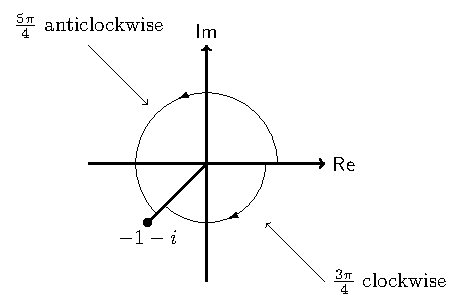
\includegraphics[scale=1]{arg}
\end{center}
We can write $\arg (z) = \frac{5\pi}{4}$ or $\arg (z)=- \frac{3\pi}{4}$ (or indeed an integer multiple of $2\pi$ added to either of these angles).




By convention we usually take $\arg (z) \in (-\pi , \pi]$.
\begin{definition}
For $z \in \C$, $z \neq 0$, we define the \emph{Principal argument of $z$} (or the \emph{Principal value of $\arg(z)$}) to be the value of $\arg (z)$ that lies in $(-\pi,\pi]$.{\marginpar{There was a typo here originally (missing minus sign in $(\pi,\pi]$)}}  We shall denote this value by $\Arg (z)$.
\end{definition}
So for $z=-1-i$ we have $\Arg (z) = - \frac{3 \pi}{4}$, while $\arg (z)$ can be taken to be any of the values
\[
\ldots, - \frac{11\pi}{4}, - \frac{3\pi}{4}, \frac{5\pi}{4}, \frac{13\pi}{4}, \ldots.
\]


\begin{definition}
The \emph{polar form} of a complex number $z$ is given by writing $z$ in the form
\[
z = r \left( \cos (\theta) + i \sin (\theta) \right),
\]
where $r , \theta \in \R$ and $r \geq 0$.
\end{definition}
The polar form of $z$ is found by setting $r = \abs{z}$ and $\theta = \arg (z)$ (any value of $\arg(z)$ will of course suffice). { Equivalently, we may write
\[
z = r e^{i \theta}
\]
(though we have yet to define the complex exponential function).}  For completeness, we should specify that the polar form of $0$ is simply $0$, since $\arg (0)$ is not defined.



\begin{definition}
Let $w=r \left( \cos( \theta) + i \sin ( \theta) \right)$ be (the polar form of) a complex number.  Then the $n^{th}$ \emph{complex roots} of $w$ are defined to be the $n$ solutions $\omega_0, \omega_1, \ldots , \omega_{n-1}$ of the equation $z^n = w$.  These roots are given by
\[
\omega_{k} = \sqrt[n]{r} \left( \cos \left( \frac{\theta+2k \pi}{n} \right) + i \sin \left( \frac{\theta + 2k\pi}{n} \right) \right),
\]
for $k=0,1,\ldots,n-1$, where $\sqrt[n]{r}$ is the (positive) $n^{th}$ real root of $r$.
\end{definition}


\begin{figure}[h]
\centering
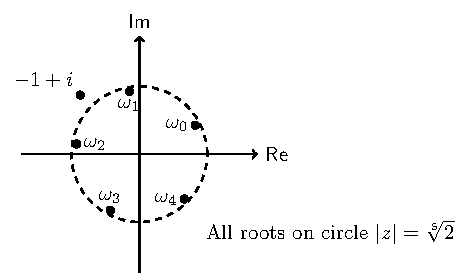
\includegraphics[scale=1]{sqrt1}
\caption{The 5\textsuperscript{th} roots of $z=-1+i$}.
\end{figure}




\begin{figure}[h]
\centering
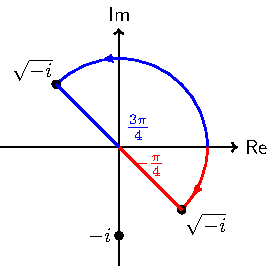
\includegraphics[scale=1]{sqrt}
\caption{The two square roots of $-i$}
\end{figure}

\begin{theorem}
Let $z_1$ and $z_2$ be nonzero complex numbers.  Then
\begin{enumerate}
\item[(i)] $\abs{z_1z_2}=\abs{z_1} \cdot \abs{z_2}$, and
\item[(i)] $\arg (z_1z_2)=\arg(z_1)+\arg(z_2)$.
\end{enumerate}
\end{theorem}
\begin{proof}
Exercise.
\end{proof}



\subsection{Complex Functions}

We now start our investigation of functions from the complex plane to itself.  First of all, note that a function $\mathbf{f}:\R^2 \to \R^2$ can be written in the form
\[
\mathbf{f}(x,y)=\left( u(x,y), v (x,y) \right)
\]
where $u,v:\R^2 \to \R$.  For example, if
\[
\mathbf{f}(x,y)=\left(x^2+y^2-2x,2y-6 \right),
\]
we have
\[
u(x,y)=x^2+y^2-2x \text{ and } v(x,y)= 2y-6.
\]





Since we have a formal definition of $\C$ as $\R^2$, we can express a function $f : \C \to \C$ as
\begin{equation*}
f(z) = f(x+iy) = u(x,y) +i v(x,y)
\end{equation*}
for all $z =x+iy \in \C$, where $u, v : \R^2 \to \R$. \ Equivalently, we could write
\[
f(z) = u(z) + i v(z),
\]
where $u,v: \C \to \R$.   In this way, we can extend our definition of real and imaginary parts from complex numbers to functions $f:\C \to \C$, writing $\Re (f) = u$ and $\Im (f) = v$.

{
\begin{itemize}
\item
Since we `define' $\C$ as $\R^2$, we can express a function $f : \C \to \C$ as
\begin{equation*}
f(z) = f(x+iy) = u(x,y) +i v(x,y)
\end{equation*}
for all $z =x+iy \in \C$, where $u, v : \R^2 \to \R$. 
\item Equivalently, we could write
\[
f(z) = u(z) + i v(z),
\]
where $u,v: \C \to \R$.  
\item Can extend our definition of real and imaginary parts from complex numbers to functions, writing $\Re (f) = u$ and $\Im (f) = v$.
\end{itemize}
}





Going in the other direction, given two functions $u:\R^2 \to \R$ and $v:\R^2 \to \R$, we can create a function $f : \C \to \C$ by \emph{defining} $f(x+iy) := u(x,y) +iv(x,y)$.
So,
\begin{center}
\emph{
 There is a correspondence between functions from the complex plane to itself, and pairs of functions from the real plane to the real line.}
 \end{center}




\begin{example}
The function \[ f: \C \to \C,\quad f(z) = \conj{z} \]
can be identified with 
\[ \mathbf{f}: \R^2 \to \R^2, \quad \mathbf{f}(x,y) = \left( u(x,y), v(x,y) \right)
\]
where
\begin{align*}
u(x,y) &= x \\
v(x,y) &= -y
\end{align*}
\end{example}
Since
\[
\conj{z} = \conj{x+iy} = x-iy = \underbrace{x}_{u(x,y)} + i \underbrace{(-y)}_{v(x,y)}.
\]


\begin{example}

Let us determine the functions $u:\R^2 \to \R$ and $v:\R^2 \to \R$ corresponding to
\begin{equation*}
h: \C \to \C, z \mapsto z^2.
\end{equation*}

{ We have
\[
(x+iy)^2 = x^2-y^2+i2xy
\]
Thus we identify $h:\C \to \C$ with $\mathbf{h}:\R^2 \to \R^2$, $\mathbf{h}(x,y) = (u(x,y), v(x,y))$  where
\begin{gather*}
u: \R^2 \to \R, (x,y) \mapsto x^2-y^2, \\
v: \R^2 \to \R, (x,y) \mapsto 2xy.
\end{gather*}
}
\end{example}


%\begin{master}
Substituting $x + iy$ for $z$ gives us
\begin{equation*}
z^2 = (x+i y)^2 = \underbrace{x^2-y^2}_{u(x,y)} +i\underbrace{ 2xy }_{v(x,y)}
\end{equation*}
%So the corresponding real function is
%\begin{equation*}
%h : \R^2 \to \R^2, (x,y) \mapsto (x^2-y^2, 2xy).
%\end{equation*}
Thus we identify $h:\C \to \C$ with $\mathbf{h}:\R^2 \to \R^2$, $\mathbf{h}(x,y) = (u(x,y), v(x,y))$  where
\begin{gather*}
u: \R^2 \to \R, (x,y) \mapsto x^2-y^2, \\
v: \R^2 \to \R, (x,y) \mapsto 2xy.
\end{gather*}
%\end{master}


\begin{example} Let us find the corresponding complex function, $f:{\mathbb C} \rightarrow {\mathbb C}$, for the function
\begin{equation*}
\mathbf{f} : \R^2 \to \R^2, (x,y) \mapsto (2y,-x)
\end{equation*}
and express it in terms of $z \in \C$.
\end{example}

%\begin{master}
\begin{solution}
The corresponding function $f:\C \to \C$ is given by
\begin{align*}
f(z)= f(x+iy)&=2y+i(-x) \\
& = 2 \Im (z) +i ( - \Re (z) ) \\
& = 2 \left( \frac{z-\overline{z}}{2i} \right)-i \left( \frac{z+\overline{z}}{2} \right) \\
&=\frac{-3i z}{2}+\frac{i\overline{z}}{2}.
\end{align*}

Thus the corresponding complex\marginpar{
Here we have used the identities $\Re (z) = \frac{1}{2} (z+\conj{z})$ and $\Im (z) = \frac{1}{2i}(z-\conj{z})$, together with the fact that $i^{-1}=-i$.
} function is
\begin{equation*}
f: \C \to \C, \ f(z)= \frac{-3i z}{2}+\frac{i\overline{z}}{2}.
\end{equation*}
\end{solution}
%\end{master}
%\vspace*{5cm}





\begin{example}
Let us do the same for the functions $\mathbf{f}:\R^2 \to \R^2$ defined by
\begin{enumerate}
\item[(i)] $\mathbf{f} (x,y) = (-2y+3,2x),$ and
\item[(ii)] $\mathbf{f}(x,y) = (x^2+y^2-2x,2y-6)$.
\end{enumerate}

\end{example}

\begin{solution}
We could follow the strategy of the previous example and use the fact that if $z=x+iy$ then
\begin{align*}
x & = \Re(z) = \frac{1}{2} \left( z+ \conj{z} \right) \\
y & = \Im (z) = \frac{1}{2i} \left( z- \conj{z} \right).
\end{align*}
Substituting these expressions for $x$ and $y$, we could then simplify and find $f(z)$. However, this is time consuming, and it is sometimes easier to look for familiar expressions in the definition of $f$.

In part (i), $\mathbf{f}$ corresponds to $f: \C \to \C$ defined by
\begin{align*}
f(z) = f(x+iy) &= -2y+3+i(2x) \\
& = 2(ix-y) + 3 \\
& = 2(ix+i^2y)+3 \\
& = 2i(x+iy)+3 \\
& = 2iz+3.
\end{align*}

In part (ii), $\mathbf{f}$ corresponds to $f:\C \to \C$ where
\[
f(x+iy) = x^2+y^2-2x+i2y-6i.
\]
With $z=x+iy$, notice that
\[
x^2+y^2=\abs{z}^2 = z \conj{z},
\]
and that
\[
-2x+i2y = -2 (x-iy) = -2 \conj{z},
\]
hence
\[
x^2+y^2-2x+i2y-6i = z \conj{z} - 2 \conj{z} -6i.
\]
Hence $f(z) = z \conj{z}-2\conj{z}-6i$ is the corresponding complex function.



\end{solution}

\begin{example}
Find the real and imaginary parts of the function $f:\C \to \C$, 
\[
f(z) = z^2-3z+4-7i.
\]
\end{example}

%\vspace*{10cm}
\begin{solution}
We are looking for $u,v:\R^2 \to \R$ so that $f(x+iy)=u(x,y)+iv(x,y)$.  To find them, we write
\[
z^2-3z+4-7i=(x+iy)^2-3(x+iy)+4-7i.
\]
After some simplification, separating into real and imaginary parts gives
\[
f(x+iy) = \underbrace{x^2-y^2-3x+4}_{u(x,y) \text{ or } \Re (f)}+i (\underbrace{2xy-3y-7}_{v(x,y) \text{ or } \Im (f)})
\]
\end{solution}


It is worth recalling that some familiar functions defined on $\R$ extend to $\C$.

\begin{definition}
\label{d:exp}
The \emph{exponential function} is the function $\exp : \C \to \C$ defined by
\[
\exp (x+iy) = \exp(x) \left( \cos (y) + i \sin (y) \right)
\]
for all complex numbers $x+iy \in \C$, where $\exp (x) (=e^x)$ is the usual (real) exponential of $x$.
\end{definition}
We shall often write $e^z$ in place of $\exp (z)$.   The trigonometric functions also extend to $\C$ via
\begin{align}
\cos (z) &= \frac{1}{2} \left( \exp (iz) + \exp (-iz) \right) \\
\sin (z) & = \frac{1}{2i} \left( \exp(iz)- \exp (-iz) \right).
\end{align}



Note that Definition~\ref{d:exp} justifies our alternative expression for the polar form of $z$.  Indeed, for any $\theta \in \R$ we have
\begin{align*}
\exp( i \theta ) =  \exp( 0+i \theta ) &= \exp (0) \left( \cos ( \theta) + i \sin (\theta) \right) \\
& = \left( \cos ( \theta) + i \sin (\theta) \right).
\end{align*}
Hence writing $z=r \left( \cos(\theta) + i \sin ( \theta ) \right)$ ( $r,\theta \in \R$ and $r>0$) is equivalent to writing\marginpar{\textbf{Note:} Since we do not yet know how to raise a (real) number to a complex power, it is not yet clear that $\exp(w+z)=\exp(w)\exp(z)$ and so on.  However, for the purposes of this module, you may assume that this identity is true (it is easily verified from the definition).}
\[
z = r \exp (i \theta).
\]



We conclude this section with some remarks about how you might go about `visualising' a complex function.  For functions $f:\R \to \R$, we usually do so by drawing the graph of $f$, that is, the subset $\set{(x,f(x)): x \in \R}$ of $\R^2$.

We cannot draw the `graph' of a function $f:\C \to \C$, as to do so would require four coordinates
\[
\set{ \Re (z), \Im (z) , \Re \left( f(z) \right), \Im \left( f(z) \right) }
\]
and thus four dimensions.  We can however view $f$ as a `transformation' of the complex plane, and examine the effect of applying $f$ to
\begin{itemize}
\item Regions (subsets) of $\C$
\item Curves in $\C$ (lines, circles etc)
\item A combination of the two.
\end{itemize}


\begin{figure}[h]
\centering
{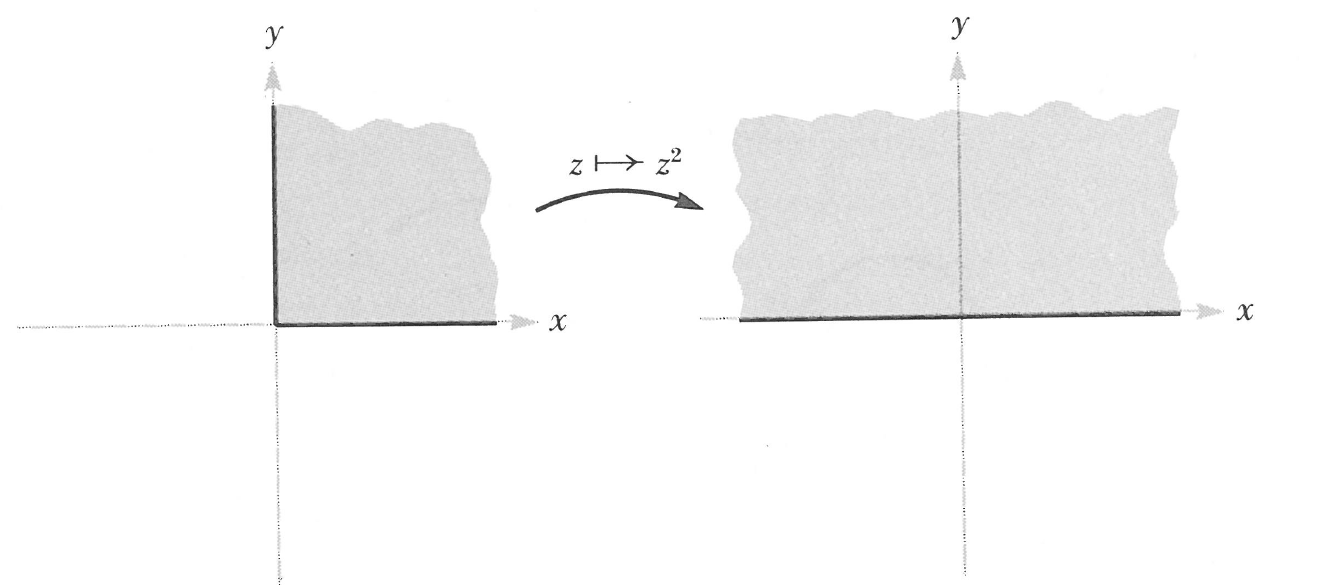
\includegraphics[scale=0.4]{z2quad}}
{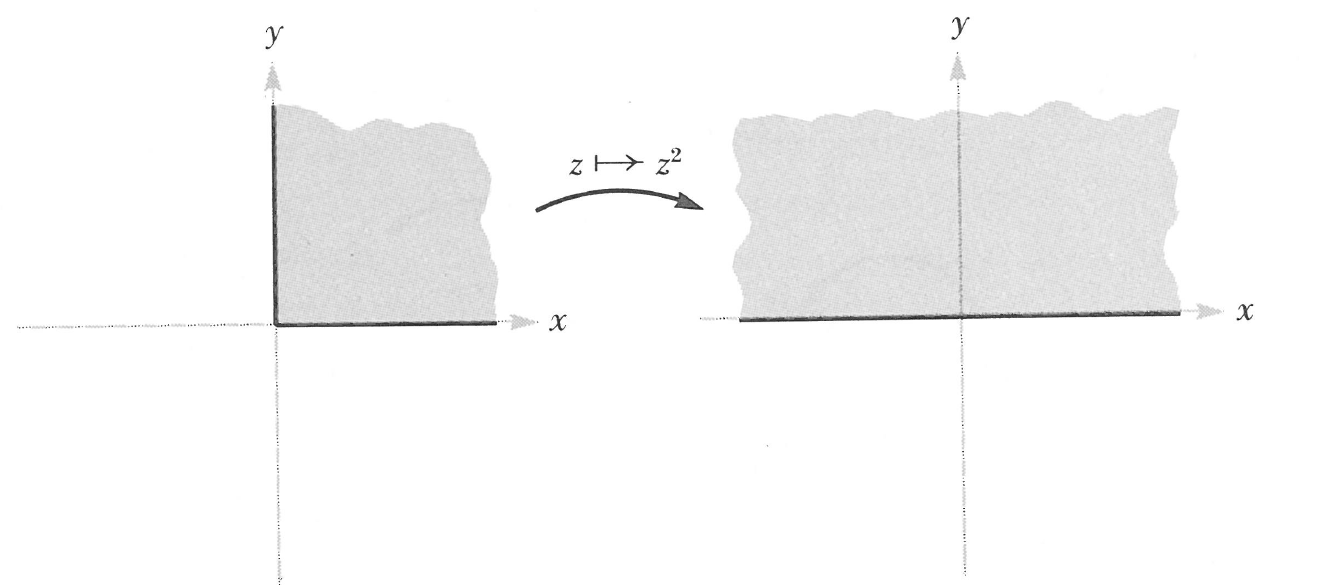
\includegraphics[scale=0.25]{z2quad}}
\caption{The image of the first quadrant under $z \mapsto z^2$.}
\label{f:z2}
\end{figure}
Figure~\ref{f:z2} indicates that the image of the first quadrant under the map $z \mapsto z^2$ is the region consisting of the first and second quadrants.  This follows from the fact that for any $z_1,z_2 \in \C$, 
\[
\arg (z_1z_2)=\arg(z_1)+\arg(z_2).
\]
Hence $\arg(z^2)=2\arg(z)$, and so if $0 \leq \arg (z) \leq \pi/2$ (i.e. $z$ is in the first quadrant), we have $0 \leq \arg (z^2) \leq \pi$ ($z^2$ lies in either the first or second quadrant).  Of course, Figure~\ref{f:z2} does not tell us anything about the modulus of $z^2$.


Figure~\ref{f:z2c} illustrates how $z \mapsto z^2$ also squares the modulus; the circle of radius $r>0$ and centre $0$ is sent to the circle of radius $r^2$ and centre $0$.  Moreover, the anticlockwise arrows on the circles indicate that if $z_2$ lies (a small distance) anticlockwise of $z_1$, then $z_2^2$ lies anticlockwise of $z_1^2$.




%\vspace*{2cm}

\begin{figure}[h]
\centering
{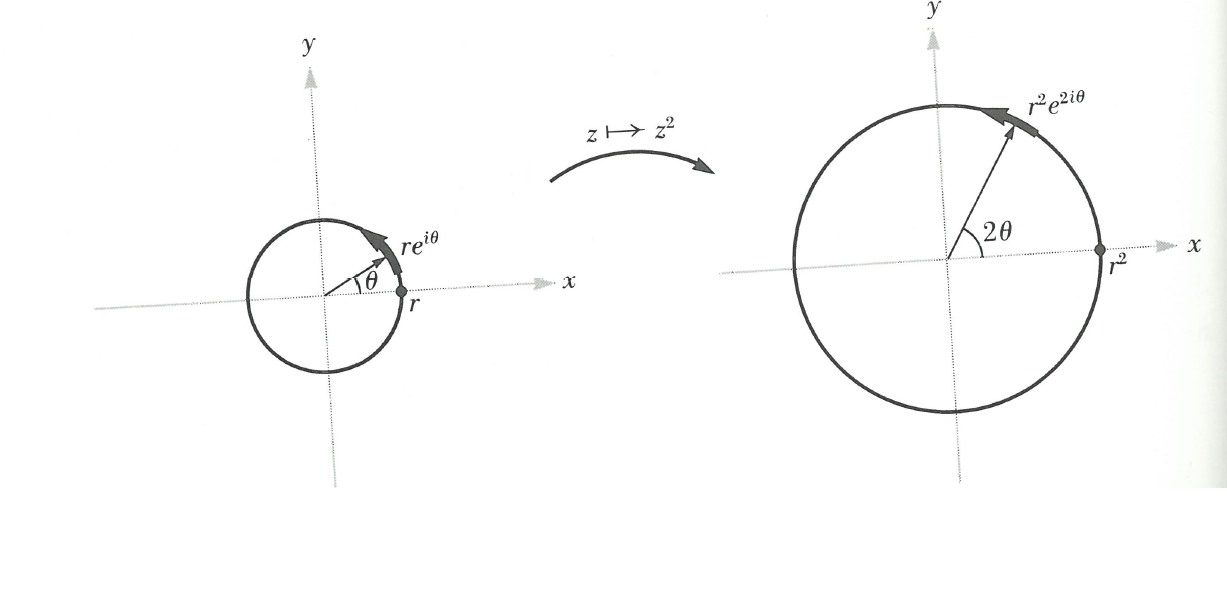
\includegraphics[scale=0.5]{z2circle}}
{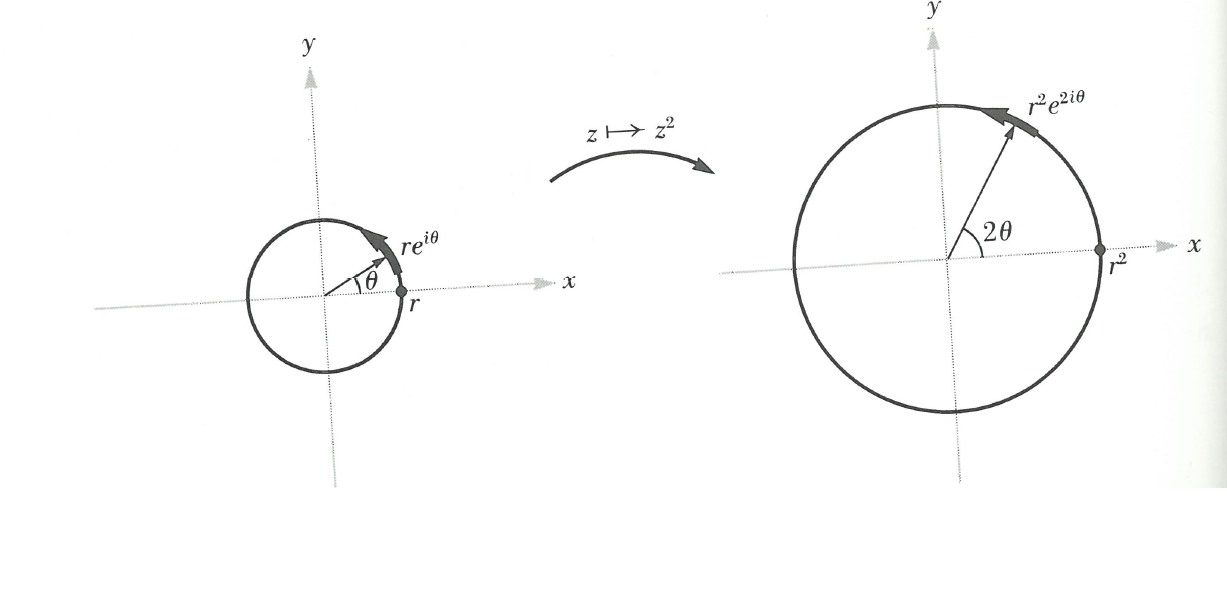
\includegraphics[scale=0.25]{z2circle}}
\caption{The effect of the map $z \mapsto z^2$ on a circle of radius $r$ centred at the origin.}
\label{f:z2c}
\end{figure}

%\vspace{2cm}

\begin{figure}[h]
\centering
{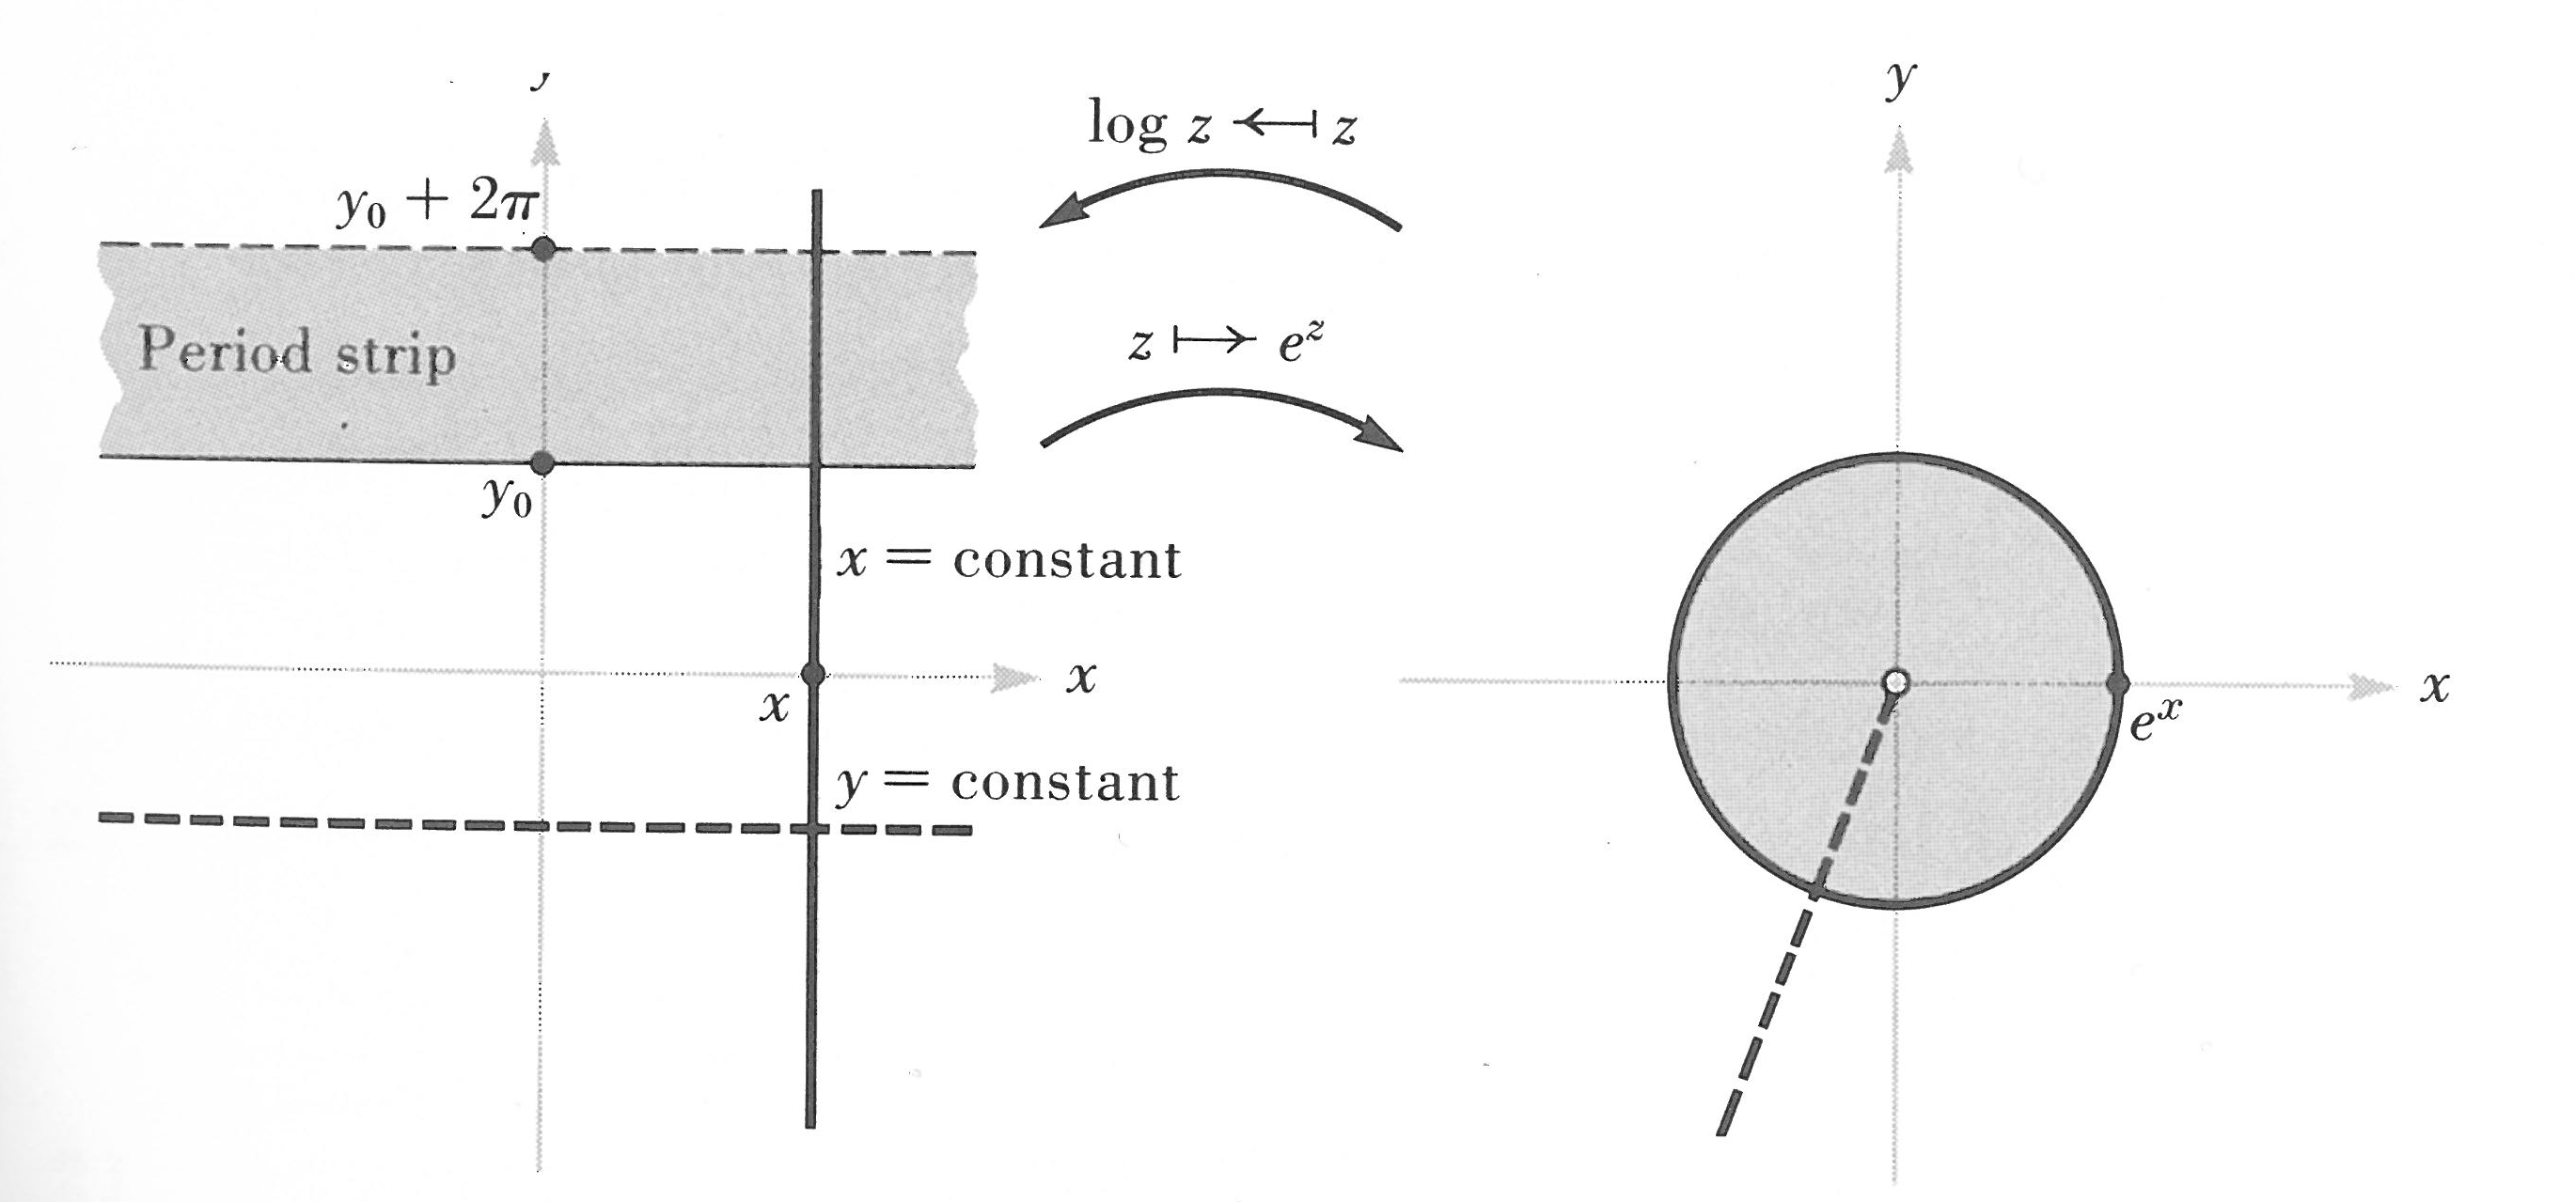
\includegraphics[scale=0.25]{expimage}}
{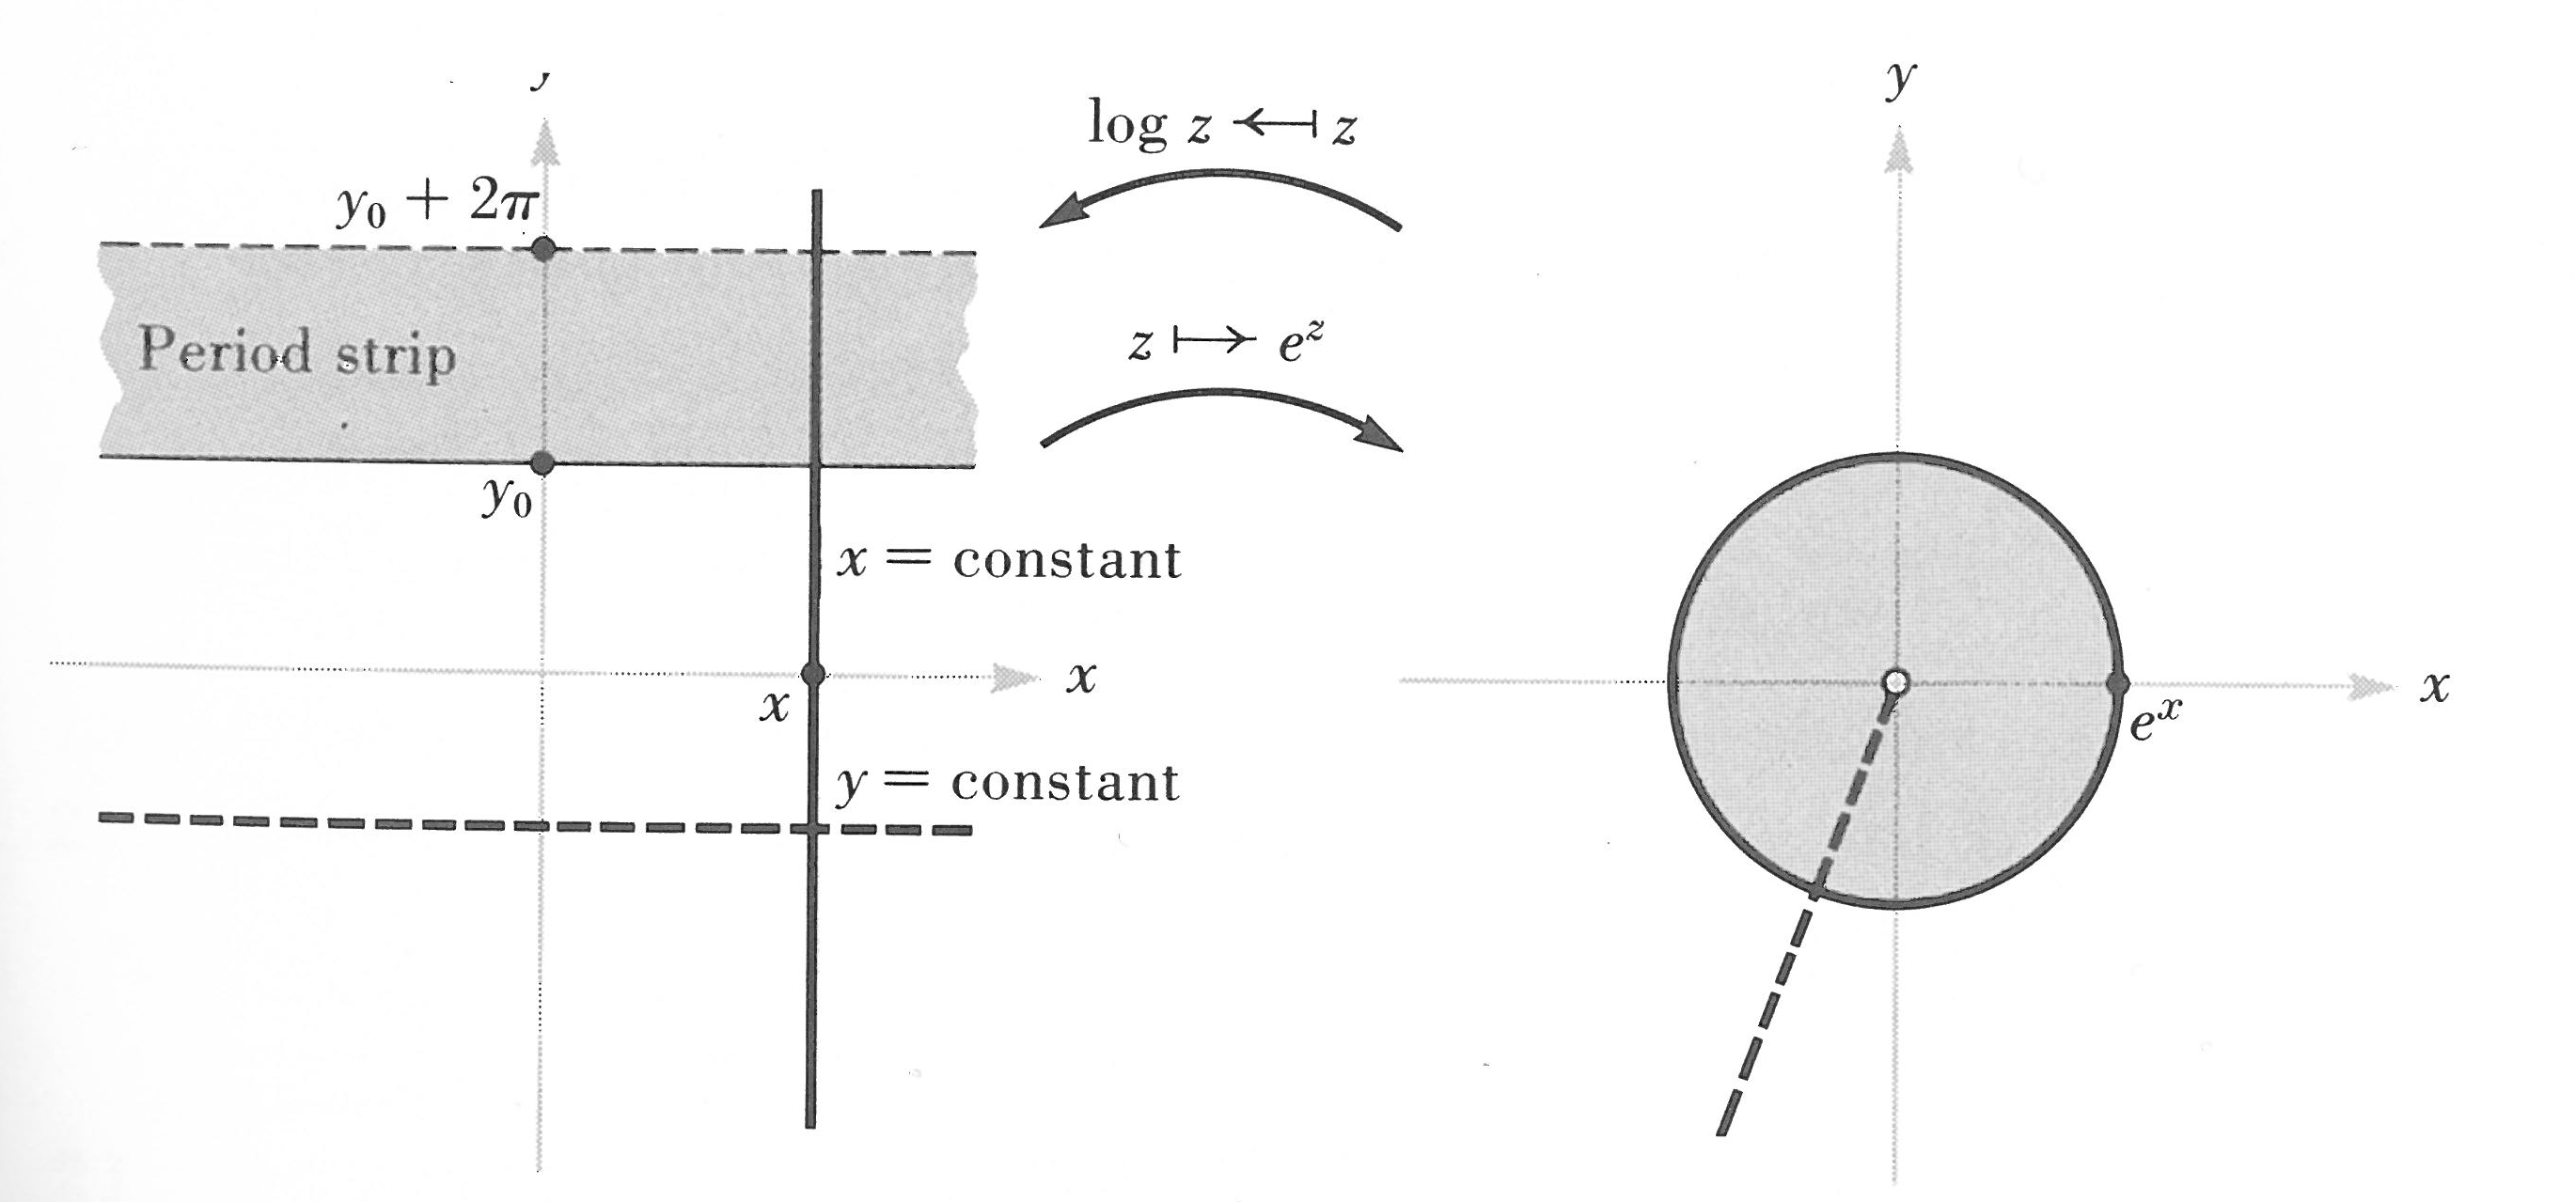
\includegraphics[scale=0.125]{expimage}}
\caption{The geometric effect of the exponential map.}
\label{f:exp}
\end{figure}

Figure~\ref{f:exp} combines the approaches of the previous examples.\marginpar{Strictly speaking this diagram is inaccurate, as some of the region to the right of the line $\Re(z)=x$ is also shaded}  Here we see that the shaded region,
\[
\set{z \in \C: \Re (z) \leq x \text{ and } y_0 \leq \Im (z) < y_0+2\pi}
\]
is sent to the shaded disc of radius $e^x$ and centre $0$.  The vertical line $\Re(z)=x$ is sent to the circle of radius $e^x$ and centre $0$, while the dashed horizontal line is sent to the `infinite ray' from $0$ indicated with another dashed line.
%\vspace{2cm}

\begin{figure}[h]
\centering
{
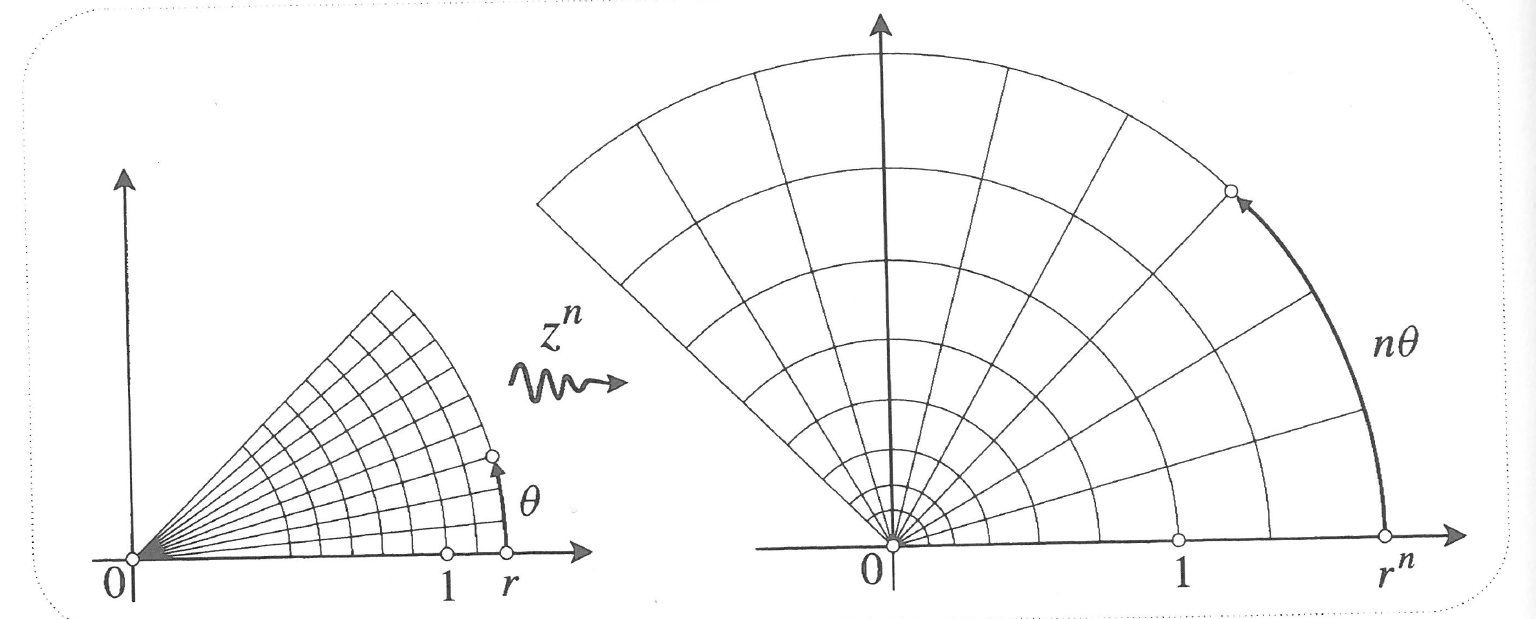
\includegraphics[scale=0.35]{znmap}
}
{
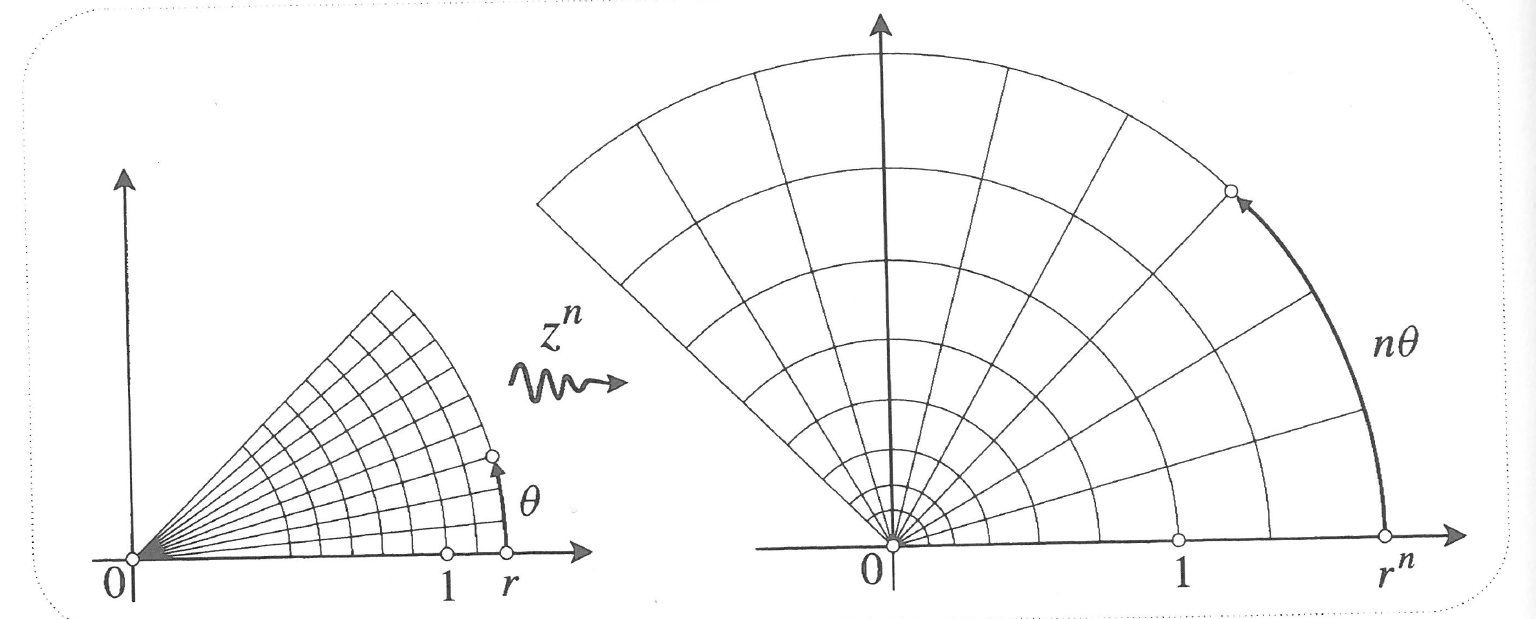
\includegraphics[scale=0.25]{znmap}
}
\caption{Another representation of $z \mapsto z^n$.  Note how this diagram indicates that the map $z \mapsto z^n$ shrinks the region $\abs{z}<1$ and enlarges the region $\abs{z}>1$.}
\label{f:zn}
\end{figure}

%\vspace*{2cm}
%Figures~\ref{f:z2},~\ref{f:z2c} and~\ref{f:exp} are from \emph{Basic Complex Analysis}, (Jerrold. E. Marsden, published by W.H. Freeman and Company, 1973).  Figure~\ref{f:zn} is from \emph{Visual Complex Analysis}, (Tristan Needham, published by Oxford University Press, 1997).

% !TEX root = main.tex

%------------------------------------------------
\section{Open Sets in $\C$}




\begin{definition}[Open Disc]
Let $w \in \C$ and let $r>0$ be some real number.  The open disc of radius $r$ centred at $w$ is defined to be the set 
\[
D(w,r):= \set{ z \in \C: \abs{z-w} <r}.
\]
\end{definition}
In other words, $D(w,r)$ is the set of all points that lie (strictly) inside the circle or radius $r$ with centre $w$.
\begin{definition}
The set of points
\[
D'(w,r) = \set{ z \in \C: 0 < \abs{z-w} < r},
\]
where $r>0$ and $w \in \C$, is called the \emph{punctured open disc} of radius $r$, centre $w$.\marginpar{This is a good place to introduce some conventions for sketching sets.  The broken circle in Figure~\ref{f:discs} around the disc indicates that the boundary is not included in this set.  The filled point $\bullet$ beside $w$ indicates that the point $w$ is included in $D(w,r)$, while the `hollow' point $\circ$ beside $w$ indicates that $w$ is not included in the punctured disc $D'(w,r)$.}
\end{definition}


Note that $D'(w,r)$ is the set obtained by removing the centre $w$ from the open disc $D(w,r)$.
\begin{figure}[h]
\centering
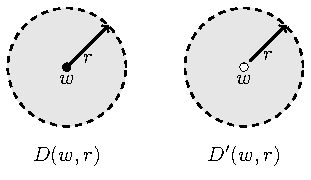
\includegraphics[scale=1]{discs}
\caption{The open disc $D(w,r)$ and punctured open disc $D'(w,r)$.}
\label{f:discs}
\end{figure}



\begin{definition}
Let $U \subseteq \C$, then we say that $U$ is an \emph{open set} if given any $w \in U$ there is some $r_w>0$ with $D(w,r_{w}) \subseteq U$.
\end{definition}
\begin{figure}[h]
\centering
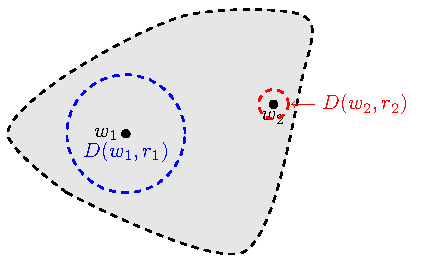
\includegraphics[scale=1]{openset}
\caption{An open set $U$ with two examples of open discs around points of $U$.  Note that the radius typically depends on the point $w$; points nearer the `edge' of $U$ will need smaller discs.}
\end{figure}



\begin{figure}[h]
\centering
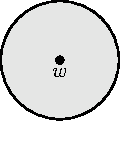
\includegraphics[scale=1]{cldisc}
\caption{An example of a set that is not open.  If we take any point $z$ on the boundary and any $r>0$, the open disc $D(z,r)$ contains points outside of the set.}
\label{f:discs2}
\end{figure}
\marginpar{The solid circle in Figure~\ref{f:discs2} indicates that the boundary is included}


\begin{example}
 The open disc $D(0,1)$ is an open set.

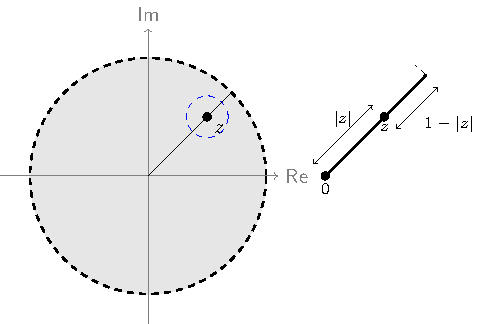
\includegraphics[scale=1]{unit_disc_full}


Let $z \in D(0,1)$.  Our goal is to find some $r>0$ so that $D(z,r) \subseteq D(0,1)$. and set $r= (1-\abs{z})/2$. Then if $w \in D(z,r)$,
\begin{align*}
\abs{w-0} & \leq \abs{w-z} + \abs{z} \\
& < \frac{1-\abs{z}}{2} +\abs{z} \\
&= \frac{1+\abs{z}}{2} < \frac{1+1}{2} = 1,
\end{align*}
which shows that $w \in D(0,1)$.

%\vspace*{2cm}


Hence $D(z,r) \subseteq D(0,1)$ and so $D(0,1)$ is open.

\end{example}



\begin{example}
 The upper-half plane $H_+$, where
\[
H_+ := \set{ z \in \C: \Im (z) > 0 }
\]
is an open set.
\begin{center}
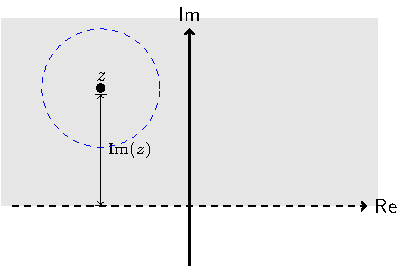
\includegraphics[scale=1]{upperhalf_full}
\end{center}
If $z \in H_+$ then $\Im (z)>0$, so we set $r = \frac{1}{2} \Im (z)$.  We want to show that $D(z,r)\subseteq H_+$, or in other words, given any $w \in D(z,r)$, we must have $\Im(w)>0$.

Let $w \in D(z,r)$, then
\[
\abs{\Im(z)-\Im(w)} \leq \abs{z-w} < r= \frac{\Im (z)}{2}.
\]
If $\Im(w)\leq 0$ then since $\Im(z)>0$ we would have
\[
\abs{\Im(z)-\Im(w)} = \Im(z) + \abs{\Im (w) } \geq \Im (z) > \frac{1}{2} \Im (z),
\]
which is a contradiction.  Hence $D(z,r) \subseteq H_+$ as required.

\end{example}



\begin{example} 
The lattice
\[
\mathbb{Z} + i\mathbb{Z} : = \set{ n + im: n,m \in \mathbb{Z} }
\]
is not open.
\begin{center}
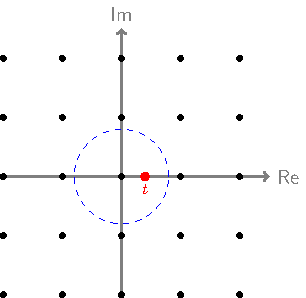
\includegraphics[scale=1]{lattice_full}
\end{center}

%\vspace*{12cm}
We shall show that the point $0 \in \mathbb{Z}+i \mathbb{Z}$ has the property that for any $r>0$, the disc $D(0,r)$ contains points in the complement of $\mathbb{Z}+i \mathbb{Z}$.\marginpar{To show that a set $S \subseteq \C$ is \emph{not} open, it is enough to find a single point $w \in S$ with the property that for any $r>0$, $D(w,r) \cap \left( \C \backslash S \right) \neq \emptyset.$}

Indeed, for any $r>0$ the point $t+0i$ where $t=\min ( \frac{1}{2} , \frac{r}{2} )$ belongs to $D(0,r)$ but not to $\mathbb{Z}+i\mathbb{Z}$.

\end{example}


\begin{note}
Some more examples of open sets include $\C \backslash \set{0}$, or indeed $\C \backslash F$ where $F$ is any finite set.  Many regions determined by \emph{strict} inequalities of real numbers are also open, for example, sets of the form
$
\set{ z \in \C: c_1<\abs{z}<c_2 }$, $\set{ z \in \C: 0 < \Arg (z) < \pi/4 }$ or $\set{z \in \C: c_1<\Re(z) < c_2 },$
where $c_1<c_2 $ are real numbers.

More examples of sets that are not open include circles, lines, curves, single points or finite sets.\marginpar{Do not use \emph{closed} to mean \emph{not open}.  In the context of analysis, closed has a different meaning.}
\end{note}
Throughout this module, we shall be mostly concerned with functions $f:U \to \C$, where $U$ is an open subset of $\C$.  

 
\subsection{Limits}
Limits in $\C$ are defined in an analogous way to those in $\R$ (and almost identically to those in $\R^2$). 

First, fix some complex number $w \in \C$.  For any $z \in \C$, the modulus $\abs{z-w}$ measures the distance between $z$ and $w$.  Note that if we write $z=x+iy$ and $w=u+iv$, then $\abs{z-w}$ is exactly the same as the Euclidean distance between $(x,y)$ and $(u,v)$ in $\R^2$.




 For a complex function $f$, what does it mean to say that $f$ approaches $L \in \C$ as $z$ approaches $w$?  \ Intuitively, we want
 \begin{center}
 $\abs{f(z)-L}$ is small whenever  $\abs{z-w}$ is small.
 \end{center}
  More formally, this can be written as
 \begin{center}
 Given any $\epsilon>0$ there is a $\delta>0$ such that
 \[
 \abs{f(z)-L} < \epsilon\text{ whenever } \abs{z-w}<\delta.
 \]
 \end{center}
 
 This definition works whenever $f$ is defined on all of $\C$, but it is not so clear how it should work when $f(z)$ is not defined near $w$. \marginpar{In other words, we want to be able to exclude points $w$ where $\abs{z-w}$ small implies $f(z)$ does not exist.} 
 
 
 \begin{definition}
 A point $w$ is a \emph{limit point} of of a set $S \subseteq \C$  if for any $\delta>0$, we have
 \[
 D'(w,\delta) \cap S \neq \emptyset.
 \]
 In other words, any punctured disc centred at $w$, no matter how small, contains at least one point of $S$.
 \end{definition}

A limit point of a set $S$ may or may not belong to $S$.  Moreover, a point $w \in S$ may or may not be a limit point of $S$.  \marginpar{If $S$ is an open set however, then any $w \in S$ is necessarily a limit point of $S$.}



\begin{example}
\begin{enumerate}
\item[(i)]  If $S=D'(w,r)$ is the punctured disc of radius $r>0$ centred at $w$, then $w$ is a limit point of $S$ that is not in $S$.
But if $R=D(w,r)$ is the complete disc, $w$ is a limit point of $R$ and $w \in R$.
\begin{center}
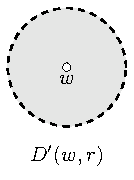
\includegraphics[scale=1]{pdisc}
\end{center}
In both cases, it is enough to note that for any $\delta>0$, the punctured disc $D'(w,\delta)$ either contains $D'(w,r)$, or else is contained in $D'(w,r)$.  In either case, the point $z:=w+s$, where $s=\min ( \frac{r}{2},\frac{\delta}{2})$ is contained in $D'(w,r) \cap D'(w, \delta)$.

\item[(ii)] If $S= \set{w}$ is a one-point set, then there are no limit points of $S$.  Indeed, for any $\delta>0$, $D'(w,\delta)$ does not contain any points of $S$ by definition.  Moreover, given any other point $z\in \C$ with $z \neq w$, the punctured disc $D'(z,\delta)$, with $\delta = \frac{1}{2} \abs{z-w}$, does not contain $w$.

\item[(iii)] The set of limit points of the open disc $S=D(w,r)$ is precisely the closed disc
\[
\set{z \in w: \abs{z-w} \leq r }.
\]
\begin{center}
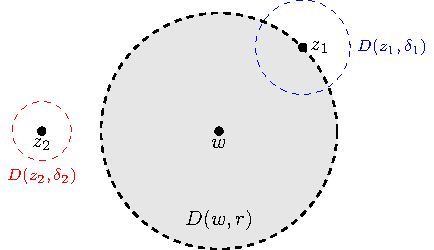
\includegraphics[scale=1]{opendisc_limitpoints} \qquad
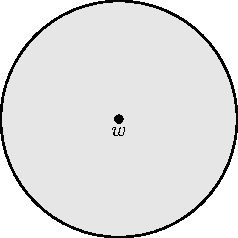
\includegraphics[scale=1]{cldisc_big}
\end{center}

If $z_1$ is a point on the boundary of $D(w,r)$, then for any $\delta>0$, $D'(z_1,\delta)$ contains points of $D(w,r)$.  If $z_2$ lies outside the boundary of $D(w,r)$, the the disc $D(z_2,\delta_2)$, where $\delta_2 = \frac{1}{2} ( \abs{w-z_2} -r)$, does not contain any points of $D(w,r)$.

\end{enumerate}
\end{example}


\begin{note}
To confuse things further, some authors require only allow points $w \in \C \backslash S$ to be limit points of $S$.  When reading textbooks or lecture notes, take care as to which definition is being used.
\end{note}


\begin{definition}
\label{d:limit}
Let $f$ be a complex function, $S \subseteq \C$ the domain of $f$,  and let $w \in \C$ be a limit point of $S$. Then we say that \[ \lim_{\substack{z \to w \\ z \in S}} f(z) = \alpha \in \C\] if given any $\epsilon >0$ there is some $\delta >0$ such that
\[ \text{ if $z \in S$ and } 0<\abs{z-w} < \delta \text{ then }\abs{f(z)-\alpha}< \epsilon.\]
\end{definition}
 
 

\begin{note}

\begin{enumerate}
\item[(i)]  Definition~\ref{d:limit} may equivalently be written in the language of open discs: 
\[
\lim_{\substack{z \to w \\ z \in S}} f(z) = \alpha
\]
if given any $\epsilon >0$ there is a $\delta >0 $ such that
\[
z \in D' (w, \delta ) \cap S \text{ implies } f(z) \in D( \alpha, \epsilon).
\]
\item[(ii)] When
\[ \lim_{\substack{z \to w \\ z \in S}} f(z) = \alpha \]
we sometimes write
\[
f(z) \to \alpha \text{ as } z \to w.
\]
\end{enumerate}

\end{note} 


\begin{example}
Is it possible to find a function $f$ for which $f(z) \to \alpha_1$ and $f(z) \to \alpha_2$ as $z \to w$, where $\alpha_1\neq\alpha_2$?
\begin{solution}
The answer, unsurprisingly, is no.  Indeed, set $\epsilon = \frac{1}{3} \abs{\alpha_1-\alpha_2}>0$.  If $f(z) \to \alpha_1$ and $f(z) \to \alpha_2$ as $z \to w$, then there would be some $\delta >0$ such that
\[
z \in D'(w,\delta) \Longrightarrow f(z) \in D'(\alpha_1 , \epsilon ) \cap D'(\alpha_2 , \epsilon).
\]
But this is impossible since clearly $D'(\alpha_1,\epsilon) \cap D'(\alpha_2 , \epsilon) = \emptyset$.
\end{solution} 
\end{example}
  
 
 
 
 \begin{comment}
This motivates our precise definition of a limit



\begin{example}
\begin{itemize}
Let $f(z)=z^3$ and $w=1+i$.
 
\end{itemize}
\end{example}

Note: it is not so clear how to adapt the definition of a limit to the case where the domain of $f$ is a proper subset of $\C$.  In order to do this, we will need to restrict our attention to a particular type of subset of $\C$ called an open set.

\begin{definition}[Limit of a function at a point of its domain]
Let $U \subseteq \C$ be an open set and $f: U \to \C$ a function defined on $U$.  For a point $w \in U$ we say that $\lim_{z \to w} f(z) = L$ if given any $\epsilon >0$ there is some $\delta >0$ such that for all $z \in U$ satisfying $\abs{z-w} < \delta$ we have $\abs{f(z)-L}< \epsilon$.
\end{definition}
We will need to generalise this definition slightly later on to allow for the case of $\lim_{z \to w} f(z)$ at a point $w \not\in \mathrm{dom} (f)$.  For example, we do not yet know how to calculate something like
\[
\lim_{z \to 0} \frac{\sin (z)}{z}
\]
(if it exists).
\end{comment}


\begin{proposition}[Algebra of limits] 
\label{p:alglimits}
Let $S\subseteq \C$ and consider functions $f,g:S \to \C.$  Suppose that $w$ is a limit point of $S$, and that $\displaystyle \lim_{\substack{z \to w \\ z \in S}} f(z) = \alpha$ and $\displaystyle \lim_{\substack{z \to w \\ z \in S}} g(z)= \beta$.  Then
\begin{enumerate}
\item[(i)] $\displaystyle \lim_{\substack{z \to w \\ z \in S}} \left( f(z) + g(z) \right) = \alpha + \beta$,
\item[(ii)] $\displaystyle \lim_{\substack{z \to w \\ z \in S}} \left( f(z)g(z) \right) = \alpha  \beta$,
\item[(iii)] If in addition $\beta \neq 0$, and $w$ is a limit point of the set $T=\set{ z \in S: g(z) \neq 0 }$, then
\[
\lim_{ \substack{z \to w \\ z \in T}} \frac{f(z)}{g(z)} = \frac{\alpha}{\beta}
\]
\end{enumerate}
\end{proposition}

\begin{proof}
The proof of this proposition is almost identical to the corresponding proof for real functions (except that $\abs{\cdot}$ refers to the modulus and not the absolute value), and is thus omitted.
\end{proof}
%\vspace*{3cm}


\subsection{Restricted Limits}

Suppose that $T$ is a subset of $S$ and $w$ is a limit point of both $T$ and $S$.  Then 
\[
 z \in D'(w, \delta) \cap T \text{ implies } z \in D' (w,\delta) \cap S.
\]
\begin{figure}[h]
\centering
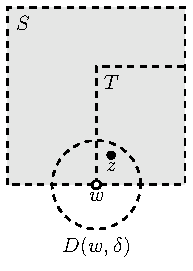
\includegraphics[scale=1]{subset1}
\caption{A subset $T$ of $S$ and a point $w$ that is a limit point of both $T$ and $S$.}
\end{figure}


It follows that
\[
 \lim_{\substack{z \to w \\ z \in S}} f(z) = \alpha \text{ implies }  \lim_{\substack{z \to w \\ z \in T}} f(z) = \alpha
\]

The second limit, where $f$ is restricted to the subset $T$ of $S$, is called a \emph{restricted limit}.   If a function has a limit at a point $w$ then all restricted limits of that function at $w$ must be the same.   In particular, 

\emph{If we have two subsets $T_1,T_2 \subseteq S$ such that 
\[
 \lim_{\substack{z \to w \\ z \in T_1}} f(z) = \alpha_1 \text{ and } \lim_{\substack{z \to w \\ z \in T_2}} f(z) = \alpha_2,
\]
with $\alpha_1 \neq \alpha_2$, then
\[
\lim_{\substack{z \to w \\ z \in S}} f(z)
\]
does not exist.
}



\begin{figure}[h]
\centering
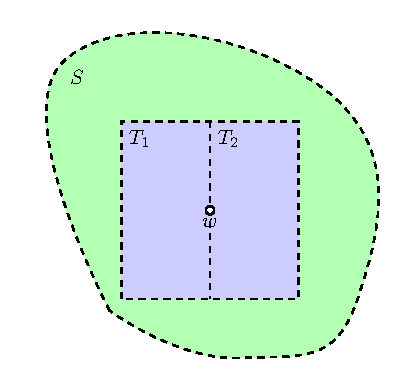
\includegraphics[scale=0.75]{subset2}\quad
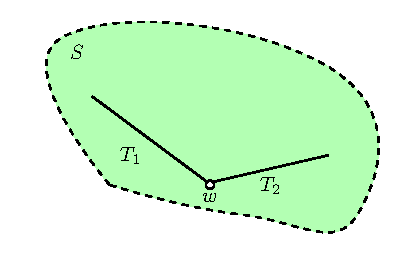
\includegraphics[scale=0.75]{subset3}
\caption{Examples of subsets $T_1$ and $T_2$ of $S$, and a common limit point $w$ of $T_1$ and $T_2$.  We shall often consider subsets of the type shown in the image on the right, where $T_1$ and $T_2$ are lines.}
\end{figure}



Let $f$ be a complex function with domain $S$ and let $w$ be a limit point of $S$.  In what follows, we shall simply write $\displaystyle \lim_{z \to w} f(z)$ in place of \[
\lim_{\substack{z \to w \\ z \in S}} f(z),
\]
and we shall reserve the second subscript for restricted limits.



\begin{example}
\label{e:rlim}
Consider the function 
\[
f: \C \backslash \set{0} \to \C, \quad f(z) = \frac{\conj{z}}{z}.
\]
Does 
$
\displaystyle \lim_{z \to 0} f(z)
$
exist?
\end{example}
\begin{note}
In future, we may simply write things like ``Let $f(z) = \dfrac{\conj{z}}{z}$'' without specifying the domain, since it is clear that this function $f$ is defined on $\C \backslash \set{0}$.
\end{note}

We shall look at two restricted limits of $f(z)$ as $z$ approaches $0$, namely the limits when $z$ is restricted to the subsets
\begin{itemize}
\item $\R \backslash \set{0}$, and
\item $i \R \backslash \set{0}$ \marginpar{Since every point on the imaginary axis is of the form $iy$ for some $y \in \R$, it makes sense to use the notation $i \R$ for this set.}
\end{itemize}
of the domain $\C \backslash \set{0}$.  Note that $0$ is a limit point of both $\R \backslash \set{0}$ and $i\R \backslash \set{0}$.
\begin{center}
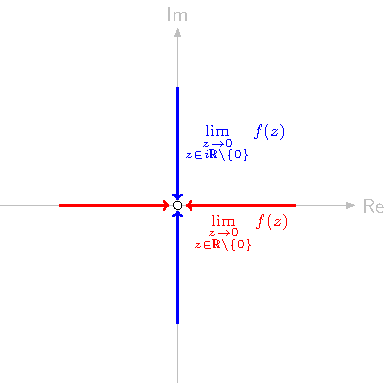
\includegraphics[scale=1]{origin_full}
\end{center}
If $z \in \R \backslash \set{0}$, then $\conj{z} = z$ and so $f(z) = \frac{\conj{z}}{z} = \frac{z}{z} =1$ on $\R \backslash \set{0}$.  Hence
\[
\rlim{z \to 0}{z \in \R \backslash \set{0} } f(z)=1.
\]
For $z \in i \R \backslash \set{0}$, we have $\conj{z}=-z$, so that $f(z)=-1$ for all such $z$, giving
\[
\rlim{z \to 0}{z \in i\R \backslash \set{0} }=-1.
\]
Since  these limits are not equal, it follows that the (unrestricted) limit $\lim_{z \to 0} f(z)$ does not exist.
%\vspace*{12cm}
\section{Continuity}

\begin{definition}
Let $S \subseteq \C$ and let $f:S \to \C$ be given.  For a point $w \in S$\marginpar{Note that the definition of continuity at $w$ only makes sense when $w$ belongs to the domain of $f$}, we say that $f$ is \emph{continuous at $w$} if $\lim_{z \to w } f(z)=f(w)$. If $f$ is continuous at all points $w \in S$ then we say that $f$ is \emph{continuous on $S$}.
\end{definition}



\begin{example}
\label{e:cts}

The functions
\begin{enumerate}
\item[(i)] $f(z) = \Re (z)$,
\item[(ii)] $f(z) = \Im (z)$, and
\item[(iii)] $f(z) = \conj{z}$
\end{enumerate}
are all continuous on $\C$.
\end{example}

\begin{solution}
Fix $w=x_0+iy_0 \in \C$ and let $\epsilon>0$ be given.  Note that for any $z=x+iy \in \C$ we have the following inequalities:
\begin{align*}
\abs{ \Re (z) - \Re (w)} = \abs{\Re (z-w)} & = \sqrt{(x-x_0)^2} \\
&\leq \sqrt{(x-x_0)^2+(y-y_0)^2} = \abs{z-w} \\
\abs{ \Im (z) - \Im (w)} = \abs{\Im (z-w)} & = \sqrt{(y-y_0)^2} \\
&\leq \sqrt{(x-x_0)^2+(y-y_0)^2} = \abs{z-w} \\
\abs{\conj{z}-\conj{w}} = \abs{\conj{z-w}} & = \abs{z-w}.
\end{align*}
Thus in all three cases, setting $\delta=\epsilon$, we get
\[
0< \abs{z-w} < \delta \Longrightarrow \abs{f(z)-f(w)} < \epsilon.
\]
\end{solution}



\begin{proposition}
\label{t:continuity}
Let $S \subseteq \C$ and let $f,g:S \to \C$ be functions that are continuous on $S$.  Then
\begin{enumerate}
\item[(i)] The function $f+g,$ where $(f+g)(z)=f(z)+g(z)$, is continuous on $S$,
\item[(ii)] The function $fg$, where $(fg)(z):=f(z)g(z)$, is continuous on $S$,
\item[(iii)] For any $\alpha \in \C$, the function $\alpha f$, where $(\alpha f)(z)=\alpha \left( f(z) \right),$ is continuous on $S$,
\item[(iv)] If $T=\set{z \in S: g(z) \neq 0 }$ then the function $ f/g$, where $ \left( \dfrac{f}{g} \right) (z)= \dfrac{f(z)}{g(z)},$ is continuous on $T$.
\end{enumerate}
\end{proposition}
\begin{proof}
Immediate from Proposition~\ref{p:alglimits}.
\end{proof}

\begin{note}
If we have
\[
f(x+iy) = u(x,y) + i v(x,y),
\]
and $w = x_0 + i y_0$ is a point in the domain of $f$, then
\[
\lim_{z \to w} f(z) = \lim_{(x,y) \to (x_0,y_0)} u(x,y)+ i \lim_{(x,y) \to (x_0,y_0)} v(x,y),
\]
provided these limits exist.  Hence
\[
f \text{ continuous at }w \Leftrightarrow u \text{ and } v \text{ continuous at } (x_0,y_0).
\]
This is useful when the real and imaginary parts of $f$ are familiar functions that we know to be continuous.
\end{note}



%------------------------------------------------
\endinput



% !TEX root = main.tex

%------------------------------------------------
\chapter[Holomorphic Functions]{Differentiability and Holomorphic Functions}
\section{The Derivative of a Complex Function}
Throughout this section, let $U$ be an open subset of $\C$.  The definition of differentiability for a function $f: U \to \C$ looks almost identical to the corresponding definition for real functions.

\begin{definition}
Let $f: U \to \C$ be a function, and let $w \in U$.  We say that $f$ is \emph{differentiable at $w$} if the limit
\begin{equation}
\label{e:diff}
\lim_{\substack{z \to 0\\ z \in \C \backslash \set{0}}} \frac{f(w+z)-f(w)}{z}
\end{equation}
exists.  When it does, we denote its value by $f'(w)$.

%If $f$ is differentiable at $w$ for all $w \in U$, we say that $f$ is \emph{holomorphic on $U$}.
\end{definition}

Since $U$ is open, the quantity (the \emph{difference quotient})
\[
\frac{f(w+z)-f(w)}{z}
\]
is defined whenever $z$ is `sufficiently small' (to ensure that $w+z \in U$ and so $f(w+z)$ is defined) but not zero (to avoid division by zero). In other words, $0$ is a limit point of the domain of the difference quotient (regarded as a function of $z$).


\begin{wrapfigure}{l}{0.5\textwidth}
\begin{framed}
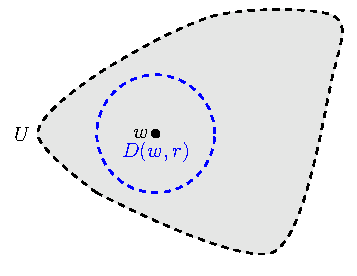
\includegraphics[scale=1]{holomorphicdomain}
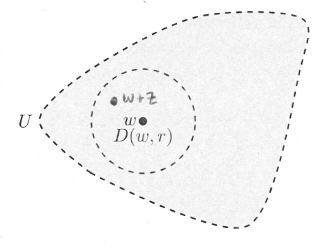
\includegraphics[scale=0.75]{openset_scan}
\caption{Since $U$ is open there is $r>0$ with $D(w,r) \subseteq U$.  For $0<\abs{z}<r$, $w+z$ lies inside this disc and hence the difference quotient is defined at $z$.}
\end{framed}
\end{wrapfigure}

 For this reason, we can again omit the second subscript and write~\eqref{e:diff} as
\[
\lim_{z \to 0} \frac{f(w+z)-f(w)}{z}
\]
without ambiguity.




\begin{example}
\label{e:diff1}
Let us investigate whether or not the function
\[
f:\C \to \C, \quad f(z)=-i\conj{z}
\]
is differentiable at any points $w \in \C$.
\end{example}

%1 page handwritten.
\begin{solution}
Fix $w \in \C$. To evaluate the limit
\[
\lim_{z \to 0} \frac{f(w+z)-f(w)}{z},
\]
we first try to simplify the expression
\[
\frac{f(w+z)-f(w)}{z}.
\]
For any $z \in \C \backslash \set{0}$, 
\[
\frac{f(w+z)-f(w)}{z} = \frac{-i\ \conj{(w+z)}-(-i)\conj{w}}{z} = -i \frac{\conj{z}}{z}.
\]
%\vspace*{8cm}
But then the limit
\[
\lim_{z \to 0} \frac{f(w+z)-f(w)}{z} = \lim_{z \to 0} -i \frac{\conj{z}}{z},
\]
is the same as the limit that we considered in Example~\ref{e:rlim}, except scaled by a factor of $-i$.  Hence this limit does not exist for the same reason; that is
\[
\rlim{z \to 0}{z \in \R \backslash \set{0}} -i \frac{\conj{z}}{z} = -i, \text{ while } \rlim{z \to 0}{z \in i\R \backslash \set{0}} -i \frac{\conj{z}}{z} = i.
\]
So $f$ is not differentiable at any point $w \in \C$.
\end{solution}



\begin{example}
\label{e:diff2}
The function $\mathbf{g}: \R^2 \to \R^2$ is defined by\marginpar{{\bf Note: } Both the real and the imaginary parts of $g$ are differentiable with respect to both $x$ and $y$ everywhere in $\R^2$.}
\[
\mathbf{g}(x,y)=(1,-x^2-y^2)\quad (x,y) \in \R^2.
\]
Find the corresponding complex function $g:\C \to \C$ and investigate where it is differentiable.
\end{example}

\begin{solution}
The corresponding function $g: \C \to \C$ is
\[
g(x+iy) = 1+i(-x^2-y^2),
\]
or equivalently,
\[
g(z) = 1-i z \conj{z}.
\]\marginpar{Since $x^2+y^2=\conj{z}z$}
Again, we fix $w \in \C$ and look at the difference quotient
\[
\frac{g(w+z)-g(w)}{z} = -i(w \frac{\conj{z}}{z}+\conj{w}+\conj{z})
\]
for $z \in \C \backslash \set{0}$.\\

As with the previous example, we have $\frac{\conj{z}}{z}$ appearing in the difference quotient, so it looks like our limit will not exist.  Again, we shall check by evaluating the restricted limits along the real and imaginary axes.

\begin{align*}
\rlim{z \to 0}{z \in \R \backslash \set{0}} -i \left( w \frac{\conj{z}}{z} + \conj{w} + \conj{z} \right) & = -i(w + \conj{w} ) \\
\rlim{z \to 0}{z \in i\R \backslash \set{0}} -i \left( w \frac{\conj{z}}{z} + \conj{w} + \conj{z} \right) & = -i (-w+\conj{w} ).
\end{align*}
These restricted limits are equal if and only if $w+\conj{w} = -w + \conj{w}$, which occurs if and only if $w=0$.  It follows that the unrestricted limit
\[
\lim_{z \to 0} \frac{g(w+z)-g(w)}{z}
\]
does not exist at any $w \in \C \backslash \set{0}$, hence $g$ is not differentiable at any of these points.

What about when $w=0$?  While the restricted limits along the real and imaginary axes are equal, this is \emph{not} enough to conclude that the unrestricted limit exists.  Indeed, we must verify this directly:
\[
\lim_{z \to 0} \frac{g(0+z)-g(0)}{z} = \lim_{z \to 0} -i \conj{z} = 0.
\]
\marginpar{Here we have used the fact that $z \mapsto \conj{z}$ is continuous (Example~\ref{e:cts}), and so limit can be found by substitution of $z=0$.}  In other words, $g$ is differentiable at $0$ (and nowhere else), with $g'(0)=0$.
%\vspace*{15cm}
\end{solution}




\begin{example}
\label{e:diff3}
Consider the function $f$ defined by $f(z)=\dfrac{1}{z}$.  At which points $w \in \C$ is $f$ differentiable?
\end{example}

\begin{solution}
Since the domain of $f$ is the (open) set $\C \backslash \set{0}$, we must necessarily restrict our attention to points $w$ in this set.  Then with $z \neq 0$, we have
\[
\frac{f(w+z)-f(w)}{z} = \frac{\left( \frac{1}{w+z} \right) - \frac{1}{w}}{z} = \frac{-1}{w(w+z)}.
\]
Since by assumption $w \neq 0$, the algebra of limits (Proposition~\ref{p:alglimits}) tells us that $-\dfrac{1}{w(w+z)} \to - \dfrac{1}{w^2}$ as $z \to 0$.  Thus $f$ is differentiable at every $w \in \C \backslash \set{0}$, with $f'(w) = -\dfrac{1}{w^2}$.
%\vspace*{6cm}
\end{solution}

\begin{example}
\label{e:diff4}
Fix $\alpha \in \C$ and let $f$ be the constant function $f(z) = \alpha$ for all $z \in \C$.  Then $f$ is differentiable at every point $w \in \C$, and satisfies $f'(w)=0$ for all $w \in \C$.
\end{example}
\begin{solution}
For any $w\in \C$, and $z \in \C \backslash \set{0}$,
\[
\frac{f(w+z)-f(w)}{z} = \frac{\alpha-\alpha}{z}=0 \to 0 \text{ as } z \to 0.
\]
\end{solution}

\begin{example}
If $f:U \to \C$ is differentiable at every point $w$ in $U$, and has $f'(w)=0$ for all $w$, is $f$ necessarily constant?
\end{example}

\begin{solution}
Not necessarily.  If $U=U_1 \cup U_2$ where $U_1$ and $U_2$ are disjoint open subsets of $\C$, and $f:U \to \C$ is defined by
\[
f(z) = \begin{cases}
0 & \text{ if } z \in U_1 \\
1& \text{ if } z \in U_2,
\end{cases}
\]
then $f'(z)$ exists and is equal to $0$ at every $z \in U$, but $f$ is non-constant.
\end{solution}
%\vspace*{5cm}

\begin{example}
\label{e:diff5}
Fix $\beta \in \C$ and let $f(z)=\beta z$.  Then $f'(w) = \beta$ for all $w \in \C$.
\end{example}

\begin{solution}
\[
\frac{f(w+z)-f(w)}{z} = \frac{\beta(w+z)-\beta w}{z}=\beta  \to 0 \text{ as } z \to 0.
\]
\end{solution}

\section{Holomorphic Functions}

\begin{definition}
Let $U \subseteq \C$ be an open set and $f:U \to \C$ a complex function.  If $f$ is differentiable at $w$ for all $w \in U$, we say that $f$ is \emph{holomorphic on $U$}.
\end{definition}
Why \emph{holomorphic} and not simply \emph{differentiable} on $U$?  One reason for this is that there are many functions $f$ that are differentiable on the real line, but fail to be differentiable throughout any open subset $U \subseteq \C$.


\begin{definition}
Let $f:U \to \C$ be a complex function and $w \in U$.  If there is some $r>0$ such that $f$ is differentiable at every point in the open disc $D(w,r)$, then $f$ is said to be \emph{holomorphic at $w$}.
\end{definition}

If a function $f$ is holomorphic at $w$, then it is differentiable at $w$, but the converse is not necessarily true.


\begin{example}
Let us examine whether or not the functions from Examples~\ref{e:diff1},~\ref{e:diff2} and~\ref{e:diff3} are holomorphic on any subsets of $\C$.

\begin{itemize}
\item $f(z)=-i\conj{z}$ is not differentiable at any $w \in \C$ and therefore not holomorphic on any $U \subseteq \C$.
%\vspace*{2cm}
\item $f(z) = 1-i z \conj{z}$ is differentiable at $0$ and nowhere else.  Since the one-point set $\set{0}$ is not an open set, there is no open subset $U \subseteq \C$ with $f$ holomorphic on $U$.
%\vspace*{3cm}
\item $f(z) = \dfrac{1}{z}$ is differentiable at every point of the (open) set $\C \backslash \set{0}$ and is therefore holomorphic on this set.
%\vspace*{3cm}
\end{itemize}

\end{example}




If $f:U \to \C$ is holomorphic on $U$, then we get a new function $f':U \to \C, \ z \mapsto f'(z)$, called the \emph{derivative of $f$}.  In other words, for $z \in U$, $f'(z)$ is defined as the limit
\[
f'(z) = \lim_{\substack{h \to 0 \\ h \in \C \backslash \set{0}}} \frac{f(z+h)-f(z)}{h}.
\]



As for differentiable functions in $\R$, we have sum, product, chain and quotient rules for holomorphic functions defined on open subsets of $\C$.

\begin{theorem}[Rules of Differentiation]
\label{t:diffrules}
Let $U$ and $V$ be open subsets of $\C$ and let $f:U \to \C$ and $g:V \to \C$ be holomorphic on $U$ and $V$ respectively.  Then
\begin{enumerate}
\item (Sum rule) $f+g$ is homomorphic on $U \cap V$ and $(f+g)'(z)=f'(z)+g'(z)$
\item (Scalar Multiples) For any $\alpha \in \C$, $(\alpha f )$ is holomorphic on $U$ and $(\alpha f)' (z) = \alpha f'(z)$
\item (Product Rule) $fg$ is holomorphic on $U \cap V$ and $(fg)'(z)=f'(z)g(z)+g'(z)f(z)$
\item (Quotient Rule) The quotient $f/g$ is holomorphic on $U \cap \set{ z \in V: g(z) \neq 0}$ and 
\[
\left( \frac{f}{g} \right) '(z) = \frac{f'(z)g(z)-f(z)g'(z)}{g(z)^2}
\]
\item (Chain Rule) $f \circ g$ is holomophic on $V \cap g^{-1}(U)$ and $(f\circ g)'(z) = f'(g(z))g'(z).$
\end{enumerate}
\end{theorem}

%\vspace*{7cm}
Since we only ever speak of a function being holomorphic on an \emph{open} subset $U \subseteq \C$, the statement of Theorem~\ref{t:diffrules} implicitly relies on the assumption that $U \cap V$, $U \cap \set{ z \in V: g(z) \neq 0 }$ and $V \cap g^{-1} (U)$ are all open whenever $U$ and $V$ are open and $f$ and $g$ are holomorphic.  These are all relatively easy to prove (the second and third rely on Proposition~\ref{p:diffimpliescontinuous}).

The proof of Theorem~\ref{t:diffrules} is very similar to that of the corresponding result for functions of a real variable, and is thus omitted.

\begin{example}
 Let $p:\C \to \C$ be a complex polynomial
\[
p(z) = \alpha_0 + \alpha_1z + \ldots + \alpha_n z^n.
\]
Then $p$ is holomorphic on $\C$.
\end{example}

\begin{solution}
We saw in Examples~\ref{e:diff4} and~\ref{e:diff5} that the functions $f(z) = \beta z$ and $g(z)= \alpha$ (where $\alpha, \beta \in \C$ are fixed), are holomorphic on $\C$ with derivatives $f'(z) = \beta$ and $g'(z)=0$ for all $z \in \C$.  Together with Theorem~\ref{t:diffrules}, this shows that $p(z)$ is holomorphic on $\C$ with derivative\marginpar{Thus complex polynomials can be differentiated using exactly the same rules as for real polynomials}
\[
p'(z) = \alpha_1 + 2\alpha_2 z + \ldots + n \alpha_n z^{n-1}.
\]
\end{solution}
\begin{note}
A similar argument shows that if $g(z) = \dfrac{1}{z^n}$ where $n >0$, then $g'(z) = -\dfrac{n}{z^{n+1}}$.
\end{note}

%\vspace*{6cm}


\begin{proposition}
\label{p:diffimpliescontinuous}
Let $f: U \to \C$ be differentiable at a point $w \in U$.  Then $f$ is continuous at $w$.
\end{proposition}

%\begin{proof}
%If $f$ is differentiable at $w$ then
%\[
%\lim_{\substack{h \to 0 \\ h \in \C \backslash \set{0}}} \frac{f(w+h)-f(w)}{h}
%\]
%exists and equals $f'(w)$.  Writing $z=w+h$, we have
%\[
%f'(w) = \lim_{ z \to w} \frac{f(z)-f(w)}{z-w}.
%\]
%Hence
%\begin{align*}
%\lim_{z \to w} \left[ f(z)-f(w) \right] &= \lim_{z \to w} \left[ \left( \frac{f(z)-f(w)}{z-w} \right) \left( z-w \right) \right] \\
%&= f'(w) \cdot 0 = 0,
%\end{align*}
%i.e., $\lim_{z \to w} f(z) = f(w)$.
%\end{proof}

\begin{example}
If $f$ is holomophic on $U$, is $f'$ holomorphic on $U$?\marginpar{In fact for holomorphic functions, the answer is yes.  This gives us an even stronger result: if $f:U \to \C$ is holomorphic on $U$, then $f$ is infinitely differentiable on $U$.  We shall return to this later on in the module.}
\end{example}
\begin{example}
In real analysis, consider $g:\R \to \R$ defined by
\[
g(x) = \begin{cases}
-x^2 & x<0 \\
x^2 & x\geq 0.
\end{cases}
\]
It is easily shown that $g$ is differentiable on $\R$ with $g'(x) = 2 \abs{x}$ for all $x \in \R$.  However, we know that $x \mapsto 2 \abs{x}$ fails to be differentiable at $0$.
\end{example}

%\vspace*{6cm}
\section{The Cauchy Riemann Equations}
Again, let $U \subseteq \C$ be open.  Suppose we are given $f:U \to \C$, then we have seen how to write $f$ as a sum of its real and imaginary parts:


\[ f(x+iy)=u(x,y)+iv(x,y) \]
for all $z=x+iy \in U$.  \

Written in terms of $z$, we have
\[
f(z) = \underbrace{\frac{f(z)+\conj{f(z)}}{2}}_{\text{Real}} + i \underbrace{\left(\frac{f(z)-\conj{f(z)}}{2i} \right)}_{\text{Real}}
\]



\begin{example}
If $u$ and $v$ are differentiable with respect to both $x$ and $y$, does it follow that $f$ is holomorphic?  
\end{example}

%\vspace*{2cm}
\begin{solution}
No.  We saw in Example~\ref{e:diff1} that
\[
f(x+iy) = 1-i (x^2+y^2),
\]
whose real and imaginary parts are differentiable everywhere in $\R^2$ with respect to both $x$ and $y$, is not differentiable at any point $w \in \C \backslash \set{0}$.
\end{solution}

For clarity, let us recall the definition of partial derivatives.



\begin{definition}
Suppose that $u: \R^2 \to \R$ is a function.  Then the \emph{partial derivatives} of $u$ with respect to $x$ and $y$ are the functions $\frac{\partial u}{\partial x}$ and $\frac{\partial u}{\partial y}$ respectively, defined via
\begin{align*}
\frac{\partial u}{\partial x} (x_0,y_0):&= \lim_{\substack{h\to 0\\h \in \R \backslash \set{0}}} \frac{u(x_0+h,y_0)-u(x_0,y_0)}{h}\\
\frac{\partial u}{\partial y} (x_0,y_0):&= \lim_{\substack{h\to 0\\h \in \R \backslash \set{0}}} \frac{u(x_0,y_0+h)-u(x_0,y_0)}{h}
\end{align*}
at the points $(x_0,y_0)$ where the limits exist.
\end{definition}

When $f=u+iv$, these partial derivatives look a bit like restricted limits of the limit that defines $f'(z)$ (or at least the real part of this limit).  Indeed, it is easy to show that
\[
\pd{u}{x} = \rlim{z \to 0}{ z \in \R \backslash \set{0} } \frac{\Re (f(w+z)) - \Re(f(w))}{z},
\]
but that
\[
\pd{u}{y} \neq \rlim{ z \to 0 }{z \in i \R \backslash \set{0} } \frac{\Re (f(w+z)) - \Re(f(w))}{z},
\]
as this time, the denominator is complex.




\begin{theorem}[Differentiability Implies the Cauchy-Riemann Equations]
\label{t:cr1}

Let $f$ be a complex-valued function defined on some open set $U$ and let $w=x_0+iy_0 \in U$.  Write
\[
f(x+iy) = u(x,y)+iv(x,y).
\]
Then if $f$ is differentiable at the point $w$ we have the following:

\begin{enumerate}
\item[(i)] The partial derivatives $\pd{u}{x}, \pd{u}{y}, \pd{v}{x}, \pd{v}{y}$ all exist at the point $(x_0,y_0) \in \R^2$ corresponding to $w$.
\item[(ii)] The partial derivatives satisfy the Cauchy-Riemann Equations at $(x_0,y_0)$:
\begin{equation}
\label{eq:cr}
\pd{u}{x} (x_0,y_0) = \pd{v}{y} (x_0,y_0),\quad \pd{u}{y} (x_0,y_0) = - \pd{v}{x} (x_0,y_0)
\end{equation}
\item[(iii)] At this point  the derivative of $f$ satisfies
\[
f'(w)= \pd{u}{x} (x_0,y_0) + i \pd{v}{x} (x_0,y_0) = \pd{v}{y} (x_0,y_0) - i \pd{u}{y} (x_0,y_0).
\]
\end{enumerate}
\end{theorem}

Before proving Theorem~\ref{t:cr1}, let us look at some examples that demonstrate how it is a powerful result.



\begin{example}
 Verify that the Cauchy-Riemann equations are satisfied by the function  $f(z)=z^2$.\\
\end{example}

Here we have
\[
f(x+iy) = \underbrace{x^2-y^2}_{u(x,y)} + i \underbrace{2xy}_{v(x,y)},
\]
and hence
\[
\pd{u}{x} = 2x = \pd{v}{y} \text{ and } \pd{u}{y} = -2y = - \pd{v}{x}.
\]
Thus~\eqref{eq:cr} holds at every $(x,y) \in \R^2$.  Moreover, we have
\[
\pd{u}{x} + i \pd{v}{x} = 2x+i2y = 2(x+iy) = 2z = f'(z),
\]
as expected.

\begin{example} 
Use the Cauchy-Riemann equations to investigate the differentiability of $f(z)=\conj{z}$.
\end{example}

This time
\[
f(x+iy) = \underbrace{x}_{u(x,y)} + i \underbrace{-y}_{v(x,y)},
\]
so that $\pd{u}{x} = 1$ while $\pd{v}{y}=-1$ and~\eqref{eq:cr} does not hold at any point $(x,y) \in \R^2$.\marginpar{Note that we need both of the equations in~\eqref{eq:cr} to hold.}
 Thus we conclude that $f(z) = \conj{z}$ is not differentiable at any point $ z \in \C$.

\begin{proof}%[Proof of Theorem~\ref{t:cr1}]
Since $f$ is differentiable at $w$ we know that
\[
\rlim{z\to 0}{z \in \C \backslash \set{0}} \frac{f(w+z)-f(w)}{z}
\]
exists and is equal to $f'(w)$.  In particular, all of corresponding restricted limits exist, and are also equal to $f'(w)$.  As before, we shall examine the restricted limits along the real and imaginary axes.

If we restrict $z$ to the nonzero real axis, then $z$ is of the form $z=h+0i$ for $h \in \R \backslash \set{0}$, and thus
\[
w+z = (x_0+h)+iy_0,
\]
which corresponds to the point $(x_0+h,y_0) \in \R^2$.  Thus the restricted limit satisfies:

%\vspace*{10cm}
\begin{align*}
f'(w) & = \rlim{h \to 0}{h \in \R \backslash \set{0}} \frac{f(w+h)-f(w)}{h} \\
& = \rlim{h \to 0}{h \in \R \backslash \set{0}} \frac{\left[ u(x_0+h,y_0)+iv(x_0+h,y_0) \right] - \left[ u(x_0,y_0)+iv(x_0,y_0) \right]}{h} \\
& \vspace*{2cm} \\
& = \left( \rlim{h \to 0}{h \in \R \backslash \set{0}} \frac{u(x_0+h,y_0)-u(x_0,y_0)}{h}  \right) +i \left(  \rlim{h \to 0}{h \in \R \backslash \set{0}} \frac{v(x_0+h,y_0)-v(x_0,y_0)}{h} \right)  \\
& = \pd{u}{x} (x_0,y_0)+i \pd{v}{x} (x_0,y_0).
\end{align*}

Hence both $\pd{u}{x}$ and $\pd{v}{x}$ exist at the point $(x_0,y_0)$, and the derivative of $f$ at $w$ satisfies
\begin{equation}
\label{eq:cr1}
\tag{$\dagger$}
f'(w) = f'(x_0+iy_0) = \pd{u}{x} (x_0,y_0)+i \pd{v}{x} (x_0,y_0).
\end{equation}
%\vspace*{7cm}

We shall now examine the restricted limit along the nonzero imaginary axis. This limit must also satisfy
\[
f'(w) = \rlim{z\to 0}{z \in i \R \backslash \set{0}} \frac{f(w+z)-f(w)}{z}.
\]
%\vspace*{3cm}
If $z \in i \R \backslash \set{0}$, then $z=0+ik$ for some $k \in \R \backslash \set{0}$, and so
\[
w+z=x_0+i(y_0+k),
\]
which corresponds to the point  $(x_0,y_0+k) \in \R^2$.

Thus
\begin{align*}
f'(w) & = \rlim{z \to 0}{z \in i\R \backslash \set{0}} \frac{f(w+z)-f(w)}{z} \\
& = \rlim{k \to 0}{k \in \R \backslash \set{0}} \frac{\left[ u(x_0,y_0+k)+iv(x_0,y_0+k) \right] - \left[ u(x_0,y_0)+iv(x_0,y_0) \right]}{ik} \\
& \vspace*{2cm} \\
& =   \rlim{k \to 0}{k \in \R \backslash \set{0}} \frac{i\ \left[ v(x_0,y_0+k)-v(x_0,y_0) \right]}{ik} +
 \rlim{k \to 0}{k \in \R \backslash \set{0}} \frac{u(x_0,y_0+k)-u(x_0,y_0)}{ik}     \\[5ex]
 & =   \rlim{k \to 0}{k \in \R \backslash \set{0}} \frac{v(x_0,y_0+k)-v(x_0,y_0)}{k} 
 -i \left( \rlim{k \to 0}{k \in \R \backslash \set{0}} \frac{u(x_0,y_0+k)-u(x_0,y_0)}{k} \right)     \\
 & = \pd{v}{y} (x_0,y_0)-i \pd{u}{y} (x_0,y_0).
\end{align*}
So $\pd{u}{y}$ and $\pd{v}{y}$ also exist at $(x_0,y_0)$, and the derivative of $f$ at $w$ also satisfies
\begin{equation}
\label{eq:cr2}
\tag{$\ddagger$}
f'(w) = f'(x_0+iy_0) = \pd{v}{y} (x_0,y_0) - i \pd{u}{y} (x_0,y_0).
\end{equation}
Equating the real and imaginary parts of the two expressions~\eqref{eq:cr1} and~\eqref{eq:cr2} for $f'(w)$ gives
\[
\pd{u}{x} (x_0,y_0) = \pd{v}{y} (x_0,y_0) \text{ and } \pd{v}{x}(x_0,y_0) = - \pd {u}{y} (x_0,y_0),
\]
which completes the proof.
%\vspace*{15cm}
\end{proof}

\section{Geometry of Derivatives for Complex-Valued Functions}
When working with differentiable functions in $\R$, it is useful to have the geometric picture of the derivative of a function $g: \R \to \R$ - for example, by considering $g'(x)$ as the slope of the tangent to the graph of $g$ at the point $(x,g(x))$.  In this section we will try to give a geometric description of the derivative of a holomorphic function $g:U \to \C$ at a point $w \in U$.  Since we cannot draw the graph of such a function, some care is needed.

Returning to the real case, consider the following graph of a function $g:\R \to \R$:
\begin{center}
%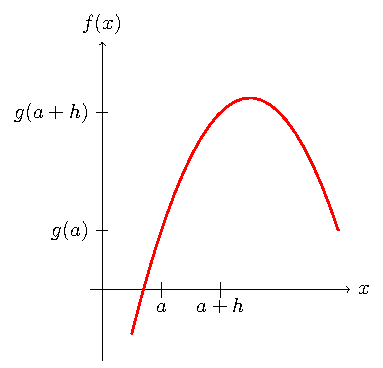
\includegraphics[scale=1]{realderivative1}
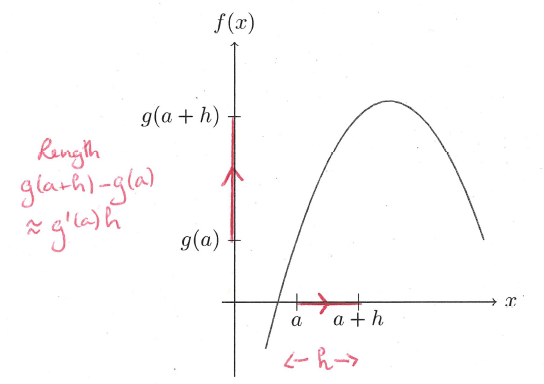
\includegraphics[scale=0.7]{derivative1_scan}
\end{center}

For sufficiently small $h$ we have
\[
\frac{g(a+h)-g(a)}{h} \approx g'(a),
\]
where $g'(a)$ is the value of the derivative of $g$ at $a$.  We can rewrite this approximation as
\[
g(a+h)-g(a) \approx g'(a) h.
\]
Now, we know that $g$ maps the interval $[a,a+h]$, of length $h$, to the interval $[g(a),g(a+h)]$ of length $g(a+h)-g(a)$  i.e. length approximately $g'(a)h$. 

In other words, $g$ moves $[a,a+h]$ to an interval from $g(a)$, and (approximately) scales it by a factor of $g'(a)$.
%\vspace*{3cm}

If $g'(a)$ is negative, then $[a,a+h]$ is approximately sent to $[g(a+h),g(a)]$. 
\begin{center}
%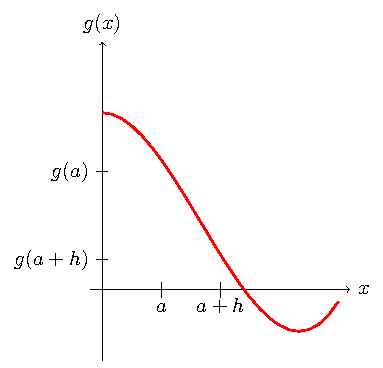
\includegraphics[scale=1]{realderivative}
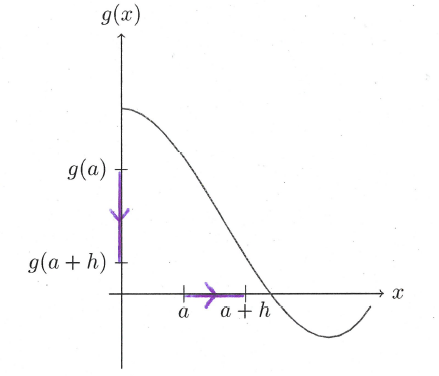
\includegraphics[scale=0.7]{derivative2_scan}
\end{center}
Then the mapping reverses the direction of the interval, i.e., sends $[a,a+h]$ to $[g(a+h),g(a)]$.  Again, the interval is scaled by a factor of $\abs{g'(a)}$, but this time, also rotated by an angle of $\pi$.  We can represent these mappings using one-dimensional figures as Figure~\ref{f:intervals} shows.

\begin{figure}[h]
\centering
%\vspace*{3cm}
%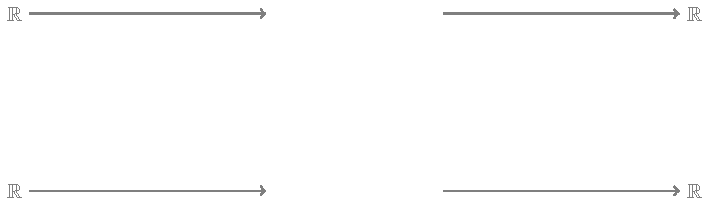
\includegraphics[scale=1]{4lines}
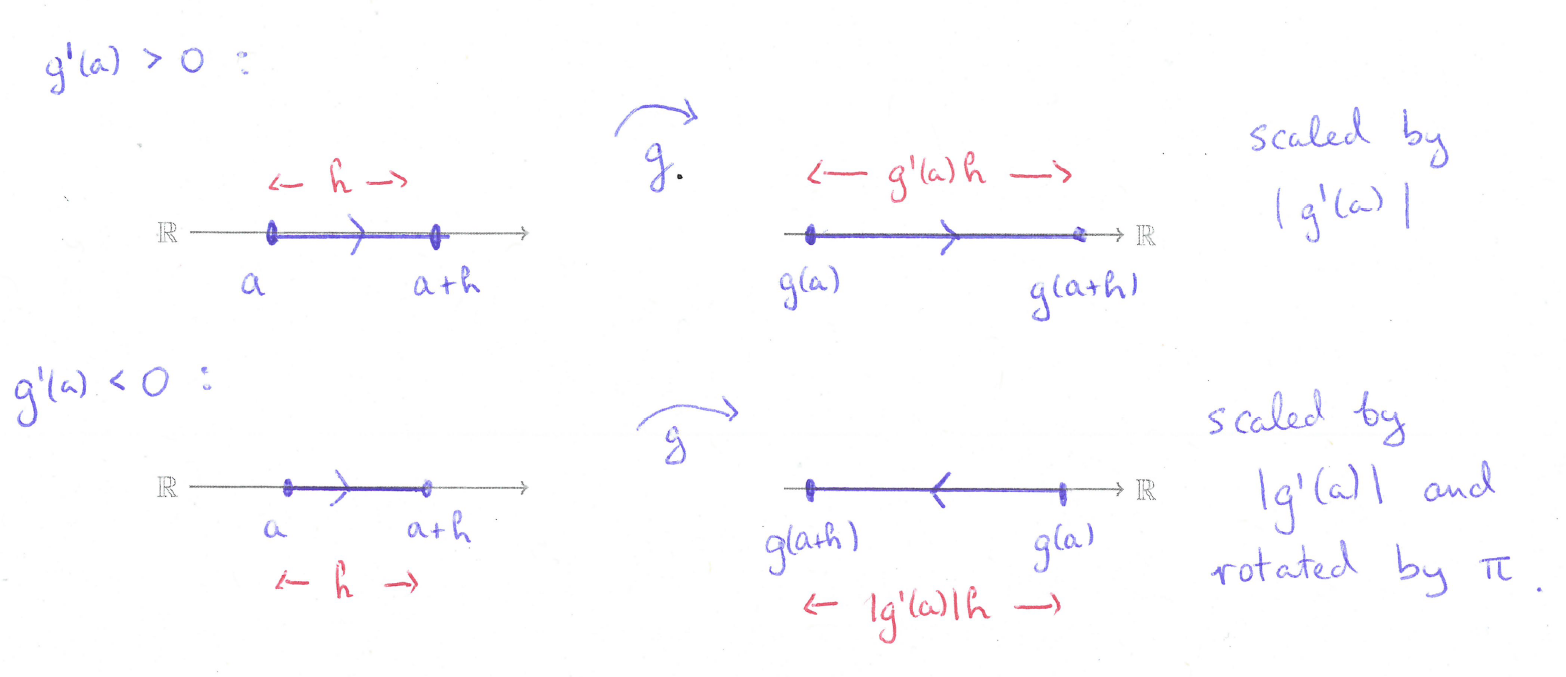
\includegraphics[scale=0.4]{4lines_full}
%\vspace*{3cm}
\caption{The image of a small interval $[a,a+h]$ under a function $g$.}
\label{f:intervals}
\end{figure}

For a complex function $f:U \to \C$, its graph is the set of points
\[
\set{ (z,f(z)): z \in U },
\]
as subset of $\C^2$.  We would need 4 coordinates to draw such a graph, which is impossible.

To describe the derivative of $f'(w)$ for a point $w \in U$, we will look at an analogy of Figure~\ref{f:intervals}.  Indeed, rather than looking at a small interval of the form $[a,a+h]$, we look at a small disk $D(w,r)$ centred at  $w$.

If $r$ is `small' and $z \in D(w,r)$ then
\[
\frac{f(w+z)-f(w)}{z} \approx f'(w),
\]
which can be rewritten as
\[
f(w+z) - f(w)\approx zf'(w).
\]
If we think of $z$ as the vector from $w$ to $w+z$, and $f(w+z)-f(w)$ as the vector from $f(w)$ to $f(w+z)$, then roughly speaking, $f$  sends $z$ to $zf'(w)$.  In other words, the vector $z$ gets moved to a vector from $f(w)$, and approximately gets multiplied by $f'(w)$, i.e.\marginpar{Again, we are using the fact that for $z_1,z_2 \in \C$, $\abs{z_1z_2} = \abs{z_1} \abs{z_2}$ and $\arg (z_1z_2) = \arg(z_1)+\arg(z_2)$.}
\begin{itemize}
\item scaled by a factor of $\abs{f'(w)}$ and
\item rotated by angle $\arg (f'(w))$ (about $f(w)$).
\end{itemize}
%\vspace*{5cm}
\begin{figure}[h]
%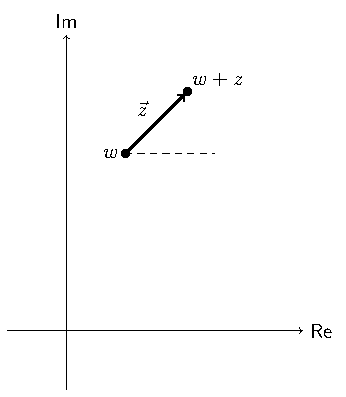
\includegraphics[scale=1]{deriv3} \qquad 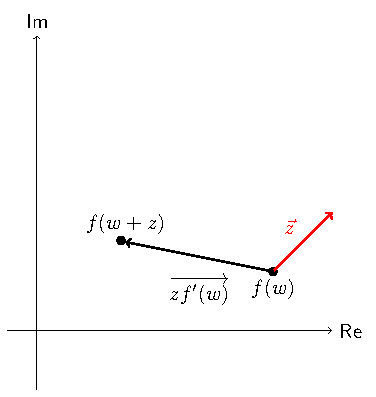
\includegraphics[scale=1]{deriv4}
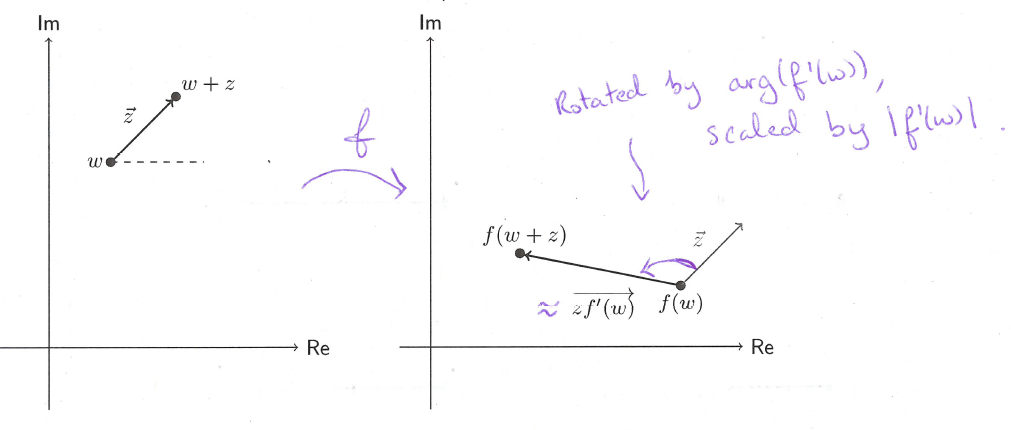
\includegraphics[scale=0.6]{deriv3_scan}
\caption{The effect of applying $f$ to points `near' $w$.  The vector $\vec{z}$ is sent to a vector from $w$, which is then scaled by $\abs{f'(w)}$ and rotated by $\arg (f'(w))$. In the diagram on the right, the angle between $\vec{z}$ and $\protect\overrightarrow{z f'(w)}$ is given by $\arg (f'(w))$.}
\end{figure}

The mapping $f$ transforms all points in $D(w,r)$ in the same way, thus
\begin{center}
\emph{$f$ maps small disks centred at $w$ to small disks centred at $f(w)$ as follows: scaling by a factor of $\abs{f'(w)}$ and rotating by angle $\arg (f'(w))$.}
\end{center}

\begin{figure}[h]
\centering
%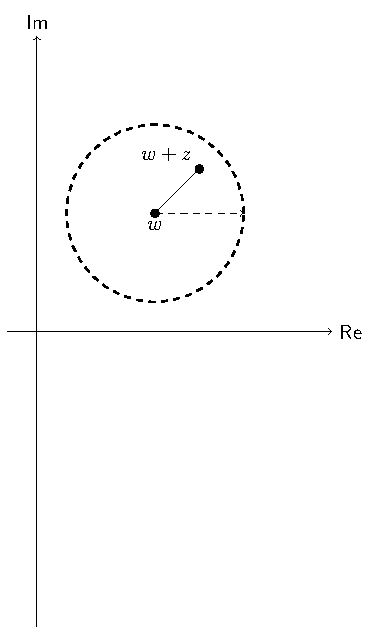
\includegraphics[scale=1]{derivative1}  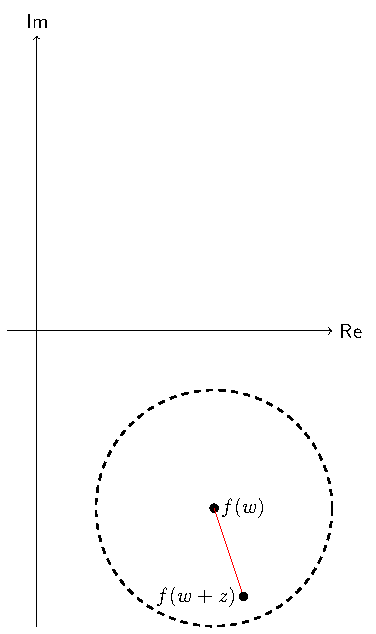
\includegraphics[scale=1]{derivative2}
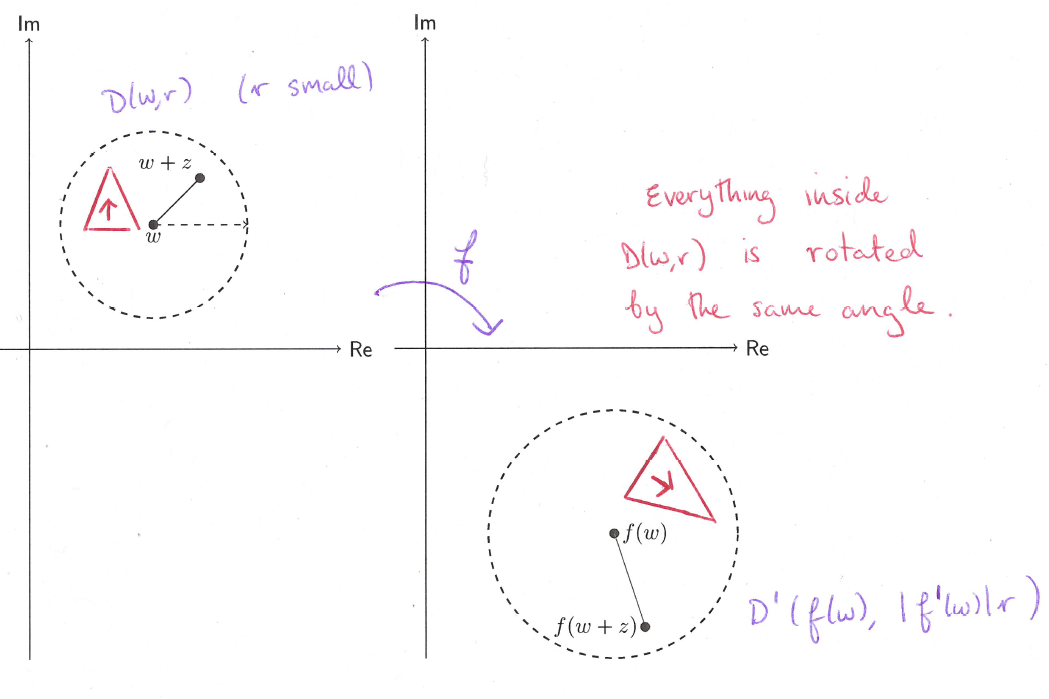
\includegraphics[scale=0.5]{deriv4_scan}
\caption{The image under $f$ of a small disc centred at $w$.}
\end{figure}

\begin{example}
Find the geometric effect of applying the function
\[
f(z)=z^2-\frac{i}{z^2}
\]
to a small disk centred at $i$.
\end{example}
%\vspace*{12cm}
Since $f$ is differentiable at $i$, the previous remarks indicate that a small disc centred at $i$ gets sent to a small disc centred at $f(i)$, where
\[
f(i) = i^2-\frac{i}{i^2} = -i+1.
\]
To determine the geometric effect of $f$ applied to this disc, we need to calculate $\abs{f'(i)}$ and $\arg (f'(i))$.  The rules of differentiation tell us that
\[
f'(z) = 2z-i \left( \frac{-2}{z^3} \right) = 2z+ \frac{2i}{z^3},
\]
and hence $f'(i) = 2i-2$, which has modulus $\abs{2i-2}=2\sqrt{2}$ and argument $3\pi/4$.

Hence a small disc at $i$ is approximately mapped to a small disc at $-1+i$, and is scaled by a factor of $2\sqrt{2}$ and rotated by an angle of $3\pi/4$  in the anticlockwise direction about $-1+i$.






\begin{figure}[h]
\centering
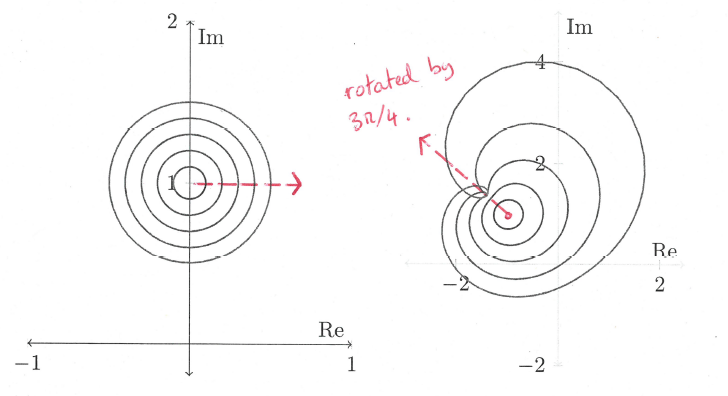
\includegraphics[scale=0.75]{parametric3_scan}
\caption{The geometric effect of applying $f(z)=z^2-\dfrac{i}{z^2}$ to small circles centred at $i$. The transformed circles are centred at $f(i)$.  As Figure~\ref{f:circles} shows, the images of the smaller circles are almost circular, but the larger ones less so.  The horizontal line from $i$ is rotated by $\arg(f'(w))$.}
\label{f:circles}
\end{figure}


\begin{example}
Find the geometric effect of applying the function $f$ defined via
\[
f(z)=\frac{z-i}{z+i}
\]
to a small disk centred at $i$.

\end{example}
%\vspace*{12cm}
This time, the disc gets mapped to a disc centred at $f(i) = \dfrac{i-i}{i+i} = 0$.  The quotient rule tells us that $f'(z) = \dfrac{2i}{(z+i)^2}$.  Hence $f'(i)=-i/2$ with modulus $1/2$ and argument $-\pi/2$.

In other words, a small disc centred at $i$ is mapped to a small disc centred at $0$, and is scaled by a factor of $1/2$ and rotated by an angle of $\pi/2$ \emph{clockwise} (since this time the argument of $f'(i)$ is negative) about $0$.

\begin{figure}[h]
\centering
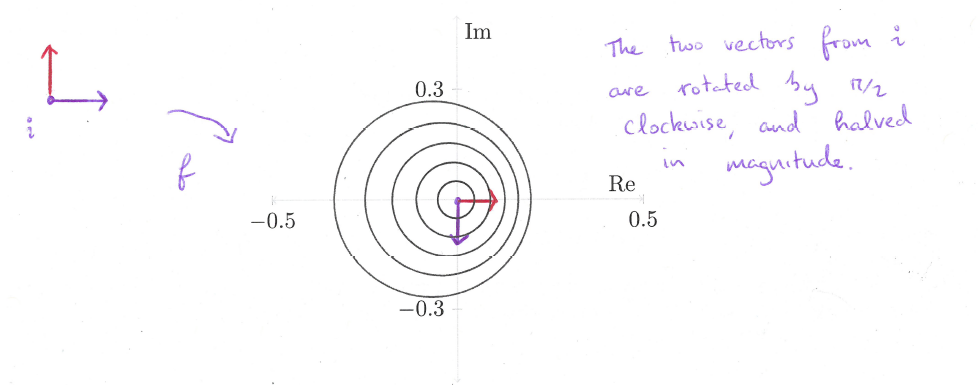
\includegraphics[scale=0.625]{parametric5_scan}
\caption{The images of circles centred at $i$ under the map $f(z)=\dfrac{z-i}{z+i}$}
\end{figure}

% !TEX root = main.tex

%------------------------------------------------
\chapter{Path Integrals in the Complex Plane}
\section{Paths}

In real analysis, we often consider the definite integral of a function $f: \R \to \R$ from a real number $a$ to another real number $b$.  Of course, on the real line, there is only one `natural' route from $a$ to $b$, namely, along the real line itself.

  There are essentially two ways of interpreting `the integral of $f$ between $a$ and $b$;' either integrating
\begin{center}
from $a$ to $b$, that is, $\int_a^b f(t) \ dt$, or \\
from $b$ to $a$, that is, $\int_b^a f(t)\ dt$.
\end{center}
Of course, these integrals have the same absolute value, but with opposite signs.


In order to make a sensible definition of integrating `between' two complex numbers $z_1$ and $z_2$, we need to take into account the fact that there are typically many routes from $z_1$ to $z_2$.  An interesting case arises when we consider paths with the same start and end-points.

\begin{figure}[h]
\centering
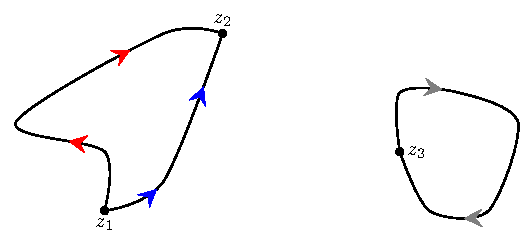
\includegraphics[scale=1]{path1}
\caption{Some examples of paths between complex numbers.}
\end{figure}

\begin{example}
\label{e:path1}
Consider the line segment $L=[z_1,z_2]$, that is, the straight line segment joining two complex numbers $z_1,z_2 \in \C$.  For an interval $[a,b] \subseteq \R$, define
\[
\gamma : [a,b] \to \C, \quad \gamma (t) = z_1 + \left( \frac{t-a}{b-a} \right) ( z_2 - z_1 ).
\]
Then the line segment $L$ is precisely the range $\gamma \left( [a,b] \right)$ of $\gamma$, with $\gamma (a) = z_1$ and $\gamma (b) = z_2$.

\end{example}

\begin{figure}[h]
\centering
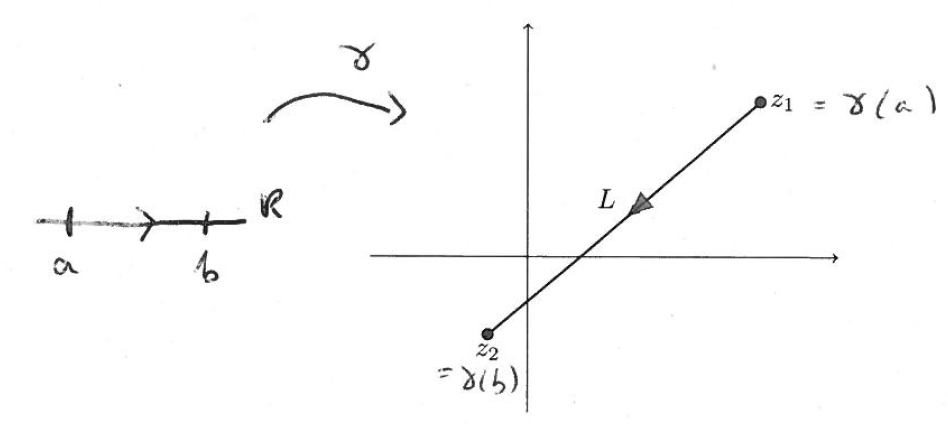
\includegraphics[scale=0.4]{param1}
\caption{The \emph{function} $\gamma:[a,b] \to \C$ describes the \emph{set} $L$, and gives it a direction (i.e. from $\gamma(a)=z_1$ to $\gamma (b)=z_2$).}
\end{figure}

The process of finding $\gamma : [a,b] \to \C$ such that each point on $L$ is of the form $\gamma (t)$, for some $t \in [a,b]$, is called a \emph{parameterisation of $L$}, and we call $t$ the \emph{parameter}.

If we think of $t$ as `time,' then as $t$ increases from $a$ to $b$, $\gamma (t)$ moves from $\gamma (a) = z_1$ to $\gamma (b) = z_2$.  It does so with `velocity'
\begin{align*}
\gamma'(t) &=\ \frac{\text{displacement}}{\text{time}} \\[2ex]
& =\  \frac{\gamma (b) - \gamma (a)}{b-a} = \frac{z_2  - z_1}{b-a}.
\end{align*}
If we think about complex numbers as points or vectors (in $\R^2$), this tells us that $\gamma (t)$ moves in the direction $z_2-z_1$ with constant speed, as you might expect.

We should clarify the definition of the derivative $\gamma'(t)$ of $\gamma(t)$ before we continue.
\begin{definition}
Let $\gamma:[a,b] \to \C$, where $[a,b] \subseteq \R$, be a complex valued function of a real variable.  Then for $t \in [a,b]$, $\gamma$ is said to be differentiable at $t$ if the limit
\[
\rlim{h \to 0}{h \in \R \backslash \set{0}} \frac{\gamma (t+h)-\gamma(t)}{h},
\]
exists.  When it does exist, we denote its value by $\gamma'(t)$, called the \emph{derivative} of $\gamma$ at $t$.
\end{definition}
Note that if $\gamma$ is written in terms of its real and imaginary parts
\[
\gamma(t) = u(t) + i v(t),
\]
where $u,v:[a,b] \to \R$, then we have
\[
\gamma'(t) = u'(t) +i v'(t),
\]
at points $t \in [a,b]$ where these derivatives exist.
%\vspace*{3cm}
\begin{example}
\label{e:path2}
A simpler parameterisation for $L=[z_1, z_2]$ is given by the function $\gamma :[0,1] \to \C$, $\gamma(t)=z_1+t(z_2-z_1)$.  Again, this path starts at $\gamma(0)=z_1$ and ends at $\gamma(1)=z_2$; it is a different \emph{function}, but describes the same \emph{set} $L$ in $\C$. This time, $\gamma'(t)=z_2-z_1$.

%\vspace*{8cm}

\end{example}

Of course, the same set can be parameterised in many different ways; in the previous example, different choices of $a$ and $b$ will give the same path (but different velocities).
%\vspace*{2cm}
\begin{example}
\label{e:path3}
Fix $R>0$ and consider the function
\[
\gamma:[0,\pi] \to \C, \gamma (t) = R \cos (t) + i R \sin (t).
\]
For all $t$, 
\[ \abs{R \cos(t)+iR \sin (t)} = \sqrt{R^2\cos^2(t)+R^2\sin^2 (t)} = R,
\]
and thus every point $\gamma(t)$ lies on the circle with centre $0$ and radius $R$.  Thus the given path consists of part of this circle.

To determine which part of the circle, we note that $\gamma$
\begin{align*}
& \text{ starts at } \gamma (0) = R\cos(0)+iR\sin(0)=R,\\
& \text{ `visits' }  \gamma \left( \pi /2 \right) = \polar{R}{\pi / 2} = iR \\
& \text{ end at }  \gamma (\pi) = \polar{R}{\pi} = -R.
\end{align*}
Thus $\gamma$ describes the upper semicircle, centre $0$ and radius $R$, traversed in the anticlockwise direction.
%\vspace*{7cm}
\begin{center}
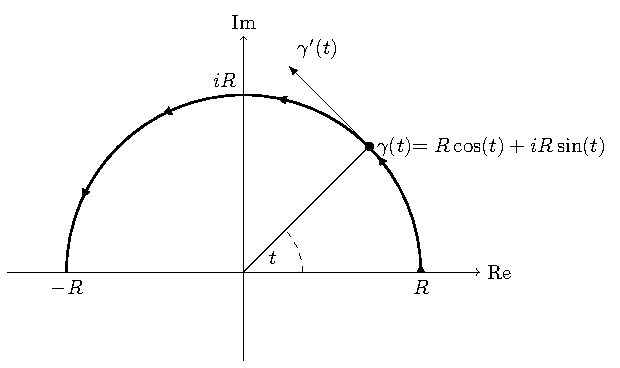
\includegraphics[scale=0.75]{semicircle0}
\end{center}
%\vspace*{6cm}
The tangent vector to this path at the point $\gamma (t)$ is given by
\begin{align*}
\gamma '(t)& = -R \sin (t) + i R \cos (t) \\
& = i^2 R \sin (t)+iR \cos (t) \\
& = i \gamma (t).
\end{align*}
Thus the tangent vector to the path at the point $\gamma (t)$ is perpendicular to the position vector $\gamma(t)$ (since multiplication by $i$ corresponds to anticlockwise rotation by $\pi/2$).
\end{example}
Note that in examples~\ref{e:path1},~\ref{e:path2} and~\ref{e:path3}, it is necessary to specify both $\gamma(t)$ and the domain of $\gamma$ in order to describe the path completely.

\begin{figure}[h]
\centering
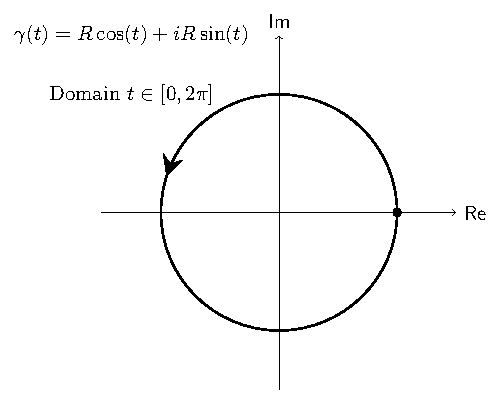
\includegraphics[scale=0.8]{path4}
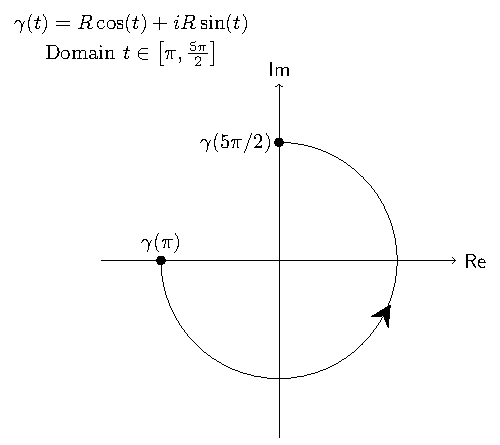
\includegraphics[scale=0.8]{path5}
\caption{Different paths defined by the function $\gamma(t) = R \cos (t) + i R \sin (t)$ when different domains are used.}
\end{figure}

\begin{definition}
A \emph{path} is a subset $\Gamma$ of $\C$ for which there is a continuous function $\gamma : [a,b] \to \C$ with
\[
\Gamma = \set{ \gamma (t) : t \in [a,b] }.
\]
The function $\gamma$ is called a \emph{parameterisation} of $\Gamma$, and we call the points $\gamma(a)$ and $\gamma(b)$ the \emph{start-} and \emph{end-points} of $\Gamma$ respectively.
\end{definition}
Note that $\Gamma$ and $\gamma$ are distinct mathematical objects: $\Gamma$ is a set and $\gamma$ is a function.  The function $\gamma$ gives a `direction' to the path $\Gamma$ ; $\Gamma$ is a path \emph{from} $\gamma (a)$ \emph{to} $\gamma(b)$. Thus when we define a path, it is usually necessary to specify a parameterisation, or at least clarify its direction, in order to avoid ambiguity.

There are typically many functions that can be used to paramterise $\Gamma$.  
Having said this, it is perfectly acceptable to define $\Gamma$ by specifying a parameterisation $\gamma$.  Thus if we say ``Consider the path defined by the function $\gamma:[a,b] \to \C$,'' then it is understood that $\Gamma = \set{ \gamma (t) : t \in [a,b] }$.


\begin{definition}
 We say that a parameterisation $\gamma:[a,b] \to \C$ of a path $\Gamma$ is \emph{smooth} if
\begin{enumerate}
\item[(i)] $\gamma$ is differentiable on $[a,b]$,
\item[(ii)] $\gamma'$ is continuous on $[a,b]$, and
\item[(iii)] $\gamma' $ is nonzero on $[a,b]$.
\end{enumerate}
A path $\Gamma$ is called smooth if there exists a smooth parameterisation of $\Gamma$.\marginpar{Informally, a smooth path is one with no corners or sharp turns.}
\end{definition}

The derivative $\gamma'(t)$, regarded as a vector, is the tangent vector to the path $\Gamma$ at the point $\gamma (t)$.

The paths in Examples~\ref{e:path1},~\ref{e:path2} and~\ref{e:path3} are all smooth.

\begin{definition}
Let $\Gamma$ be a path with smooth parameterisation $\gamma: [a,b] \to \C$.  Then the \emph{reverse} of $\Gamma$ is the path $\tilde{\Gamma}$ consisting of the same set of points as $\Gamma$, but traversed in the opposite direction.  The path $\tilde{\Gamma}$ may be parameterised by the function $\tilde{\gamma} : [a,b] \to \C$ where
\[
\tilde{\gamma} (t) = \gamma (a+b-t) \quad \text{for all } t \in [a,b].
\]
\end{definition}
\begin{comment}
\begin{note}
Since we have defined $\Gamma$ to be a set of points, there is nothing to distinguish $\Gamma$ and $\tilde{\Gamma}$ - they both define the same subset of $\C$.  Hopefully this will not cause too much confusion.
\end{note}
\end{comment}

Note that if we define the start- and end-points of $\Gamma$ to be
 \[ \gamma (a) = z_1, \quad \gamma (b) = z_2 \] 
 then
\begin{align*}
\tilde{\gamma} (a) & = \gamma (a+b-a) = \gamma (b) = z_2 \\
\tilde{\gamma} (b) & = \gamma (a+b-b) = \gamma (a) = z_1.
\end{align*} 
Thus $\tilde{\Gamma}$ starts at $z_2$ and ends at $z_1$.  Moreover, if $t \in [a,b]$ then $a \leq a+b-t \leq b$, and so $\tilde{\gamma} (t)$ describes a point on the original path $\Gamma$ (i.e. $\tilde{\Gamma}$ is the same set as $\Gamma$).

The tangent vector is given by
\[
\tilde{\gamma} ' (t) = \frac{d}{dt} \gamma (a+b-t) = \gamma'(a+b-t) \frac{d}{dt}(a+b-t) = - \gamma'(a+b-t).
\]
In other words, at any point $z = \tilde{\gamma} (t) = \gamma (a+b-t)$ on the path $\Gamma$, the tangent vector to this path at $z$, when travelling in the reverse direction, points in the opposite direction to the tangent vector obtained when travelling in the original direction, as expected.
 \begin{note}
 Moreover, for each $t \in [a,b]$:
 

  \[ \tilde{\gamma} (t) \text{ lies on } \Gamma .\]  

For $t \in [a,b]$, 
\[
\tilde{\gamma} ' (t) = \begin{master} \gamma' (a+b-t) (-1) = - \gamma' (a+b-t). \end{master}
\]
\end{note}
%\vspace*{10cm}

Thus the definition of $\tilde{\gamma}$ ensures that $\tilde{\Gamma}$ is indeed the curve from $z_2$ to $z_1$ along the original path $\Gamma$, but traversed in the opposite direction.

\begin{example}
Let us find the reverse of the paths considered in Examples~\ref{e:path2} and~\ref{e:path3}.

\begin{itemize}
\item $L=[z_1, z_2 ] $, parameterised by $\gamma:[0,1] \to \C$, $\gamma (t) = z_1 + t ( z_2 - z_1 )$.
It is clear that the reverse of $L$ is the line segment $\tilde{L}=[z_2,z_1]$, i.e. the same line segment taken from $z_2$ to $z_1$.  We may parameterise $\tilde{L}$ with the function $\tilde{\gamma}:[0,1] \to \C$, where
\begin{align*}
\tilde{\gamma} (t) & = \gamma (0+1-t ) \\
& = z_1 + (1-t)(z_2-z_1) \\
& = z_2+t(z_1-z_2).
\end{align*}
On examining the equation for $\tilde{\gamma} (t)$, it is clear that this function describes the path that starts at $z_2$ and travels in the direction $(z_1-z_2)$.
\item  $\Gamma$ the semicircle parameterised by $\gamma:[0,\pi] \to \C$ , $\gamma (t) = R \cos (t) + i R \sin (t)$. 

In this case $\tilde{\Gamma}$ is the clockwise semicircular arc from $-R$ to $R$ via $iR$.  We may parameterise $\tilde{\Gamma}$ using $\tilde{\gamma}:[0,\pi] \to \C$, where
\begin{align*}
\tilde{\gamma} (t) & = \gamma ( \pi-t) \\
& = R \cos ( \pi-t)+iR \sin (\pi-t) \\
& = -R \cos (t) + i R \sin (t).
\end{align*}
Note that $\tilde{\gamma} (t)$ is $\gamma (t)$ reflected through the imaginary axis; and thus the path $\tilde{\Gamma}$ is the reflection of the path $\Gamma$ in the imaginary axis.
%\vspace*{9cm}

\end{itemize}
\end{example}

We shall often need to consider the paths that we obtain from joining smooth paths together.  Note that the resulting path may fail to be smooth, e.g., if there is a `corner' at the point where they meet.

Suppose we have two or more (smooth) paths $\Gamma_1,\ \Gamma_2$ etc., parameterised by $\gamma_1:[a_1,b_1] \to \C$ and $\gamma_2:[a_2,b_2] \to \C$, and suppose that the end-point of $\Gamma_1$ is the same as the start-point of $\Gamma_2$, i.e. $\gamma_1(b_1)=\gamma_2(a_2)$.

\begin{figure}[h]
\centering
\begin{framed}
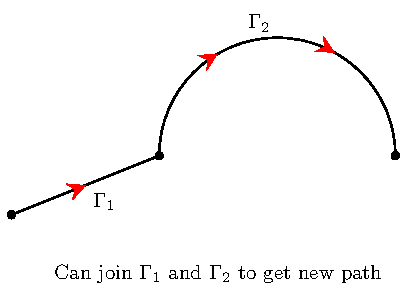
\includegraphics[scale=0.8]{join1}
%\end{framed}
\hspace{2cm}
%\begin{framed}
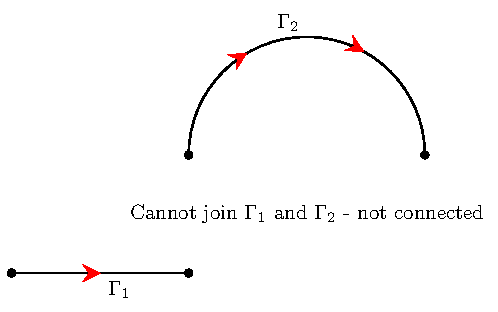
\includegraphics[scale=0.8]{join3}
%\end{framed}
\vspace*{1cm}
%\begin{framed}
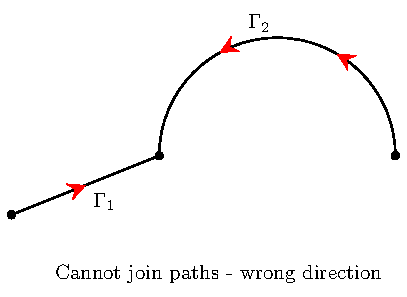
\includegraphics[scale=0.8]{join2}
\end{framed}
\end{figure}

The curve obtained from $\Gamma_1 \cup \Gamma_2 $ certainly looks like a path, but how do we make this precise?  In other words, can we describe this curve as the image of some continuous $\gamma: [a,b] \to \C$?
\begin{figure}[h]
\centering
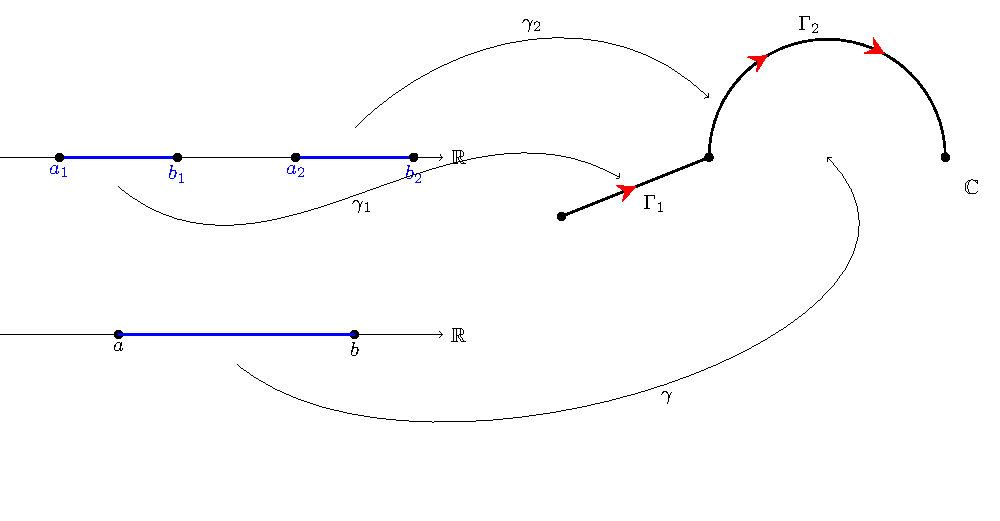
\includegraphics[scale=0.75]{join4}
\caption{We have two functions $\gamma_1:[a_1,b_1] \to \C$ and $\gamma_2:[a_2,b_2] \to \C$ parameterising $\Gamma_1$ and $\Gamma_2$ respectively.  We want a single continuous function $\gamma:[a,b] \to \C$ parameterising $\Gamma_1 \cup \Gamma_2$}.
\end{figure}
To do this, we first move $[a_2,b_2]$ to an interval from $b_1$ and then reparameterise $\Gamma_2$.  For $t \in \R$, let $\alpha(t)=  t-(a_2-b_1)$, so that $\alpha$ maps $[a_2,b_2]$ bijectively to $[b_1,b_1+b_2-a_2]$.
\begin{figure}[h]
\centering
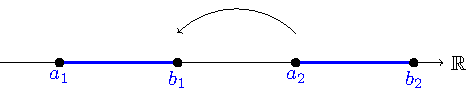
\includegraphics[scale=1]{join5}
\end{figure}
%\vspace*{5cm}
Now, parameterise $\Gamma_2$ using the function $\gamma_{1+2}:[b_1,b_1+b_2-a_2] \to \C$, where
\[
\gamma_{1+2} (t) = \gamma_2 ( \alpha^{-1} (t) ) = \gamma_2 (t+a_2-b_1)
\]
for all $t \in [b_1,b_1+b_2-a_2]$.
\begin{definition}
Suppose that $\Gamma_1$ and $\Gamma_2$ are two paths parameterised by $\gamma_1:[a_1,b_1] \to \C$ and $\gamma_2:[a_2,b_2] \to \C$ respectively, such that $\gamma_1(b_1) = \gamma_2 (a_2)$.  Then we define the \emph{join} of $\Gamma_1$ and $\Gamma_2$ to be the path $\Gamma_1+\Gamma_2$ parameterised by $\gamma_{1+2}:[a_1,b_1+b_2-a_2] \to \C$, where
\[
\gamma_{1+2} (t) = \begin{cases}
\gamma_1 (t) & t \in [a_1,b_1] \\
\gamma_2 (t-b_1+a_2) & t \in [b_1,b_1+b_2-a_2].
\end{cases}
\]
\end{definition}


If we have another path $\Gamma_3$ we can join $\Gamma_3$ to $\Gamma_1+\Gamma_2$ to get $\Gamma_1+\Gamma_2+\Gamma_3$ and so on.

\begin{definition}
A \emph{contour} is a path which is the join of finitely many smooth paths.
\end{definition}

\begin{figure}[h]
\centering
\includegraphics[scale=1]{contour1}
\caption{A contour $\mathcal{C}$ constructed from the join of smooth paths $\Gamma_1,\Gamma_2,\ldots,\Gamma_5$.  Note that $\mathcal{C}$, considered as a path in its own right, need not be smooth.}
\end{figure}


\begin{definition}
Let $\Gamma$ be a smooth path parameterised by $\gamma:[a,b] \to \C$.  Then the \emph{length} $\ell ( \Gamma)$ of $\Gamma$ is defined to be
\[
\ell ( \Gamma ) : = \int_a^b \abs{ \gamma '(t) } \ dt.
\]
For a contour $\mathcal{C} = \Gamma_1+\Gamma_2 + \ldots + \Gamma_n$, where $\Gamma_1,\Gamma_2, \ldots , \Gamma_n$ are smooth, we define the \emph{length} $\ell ( \mathcal{C} )$ of $\mathcal{C}$ to be
\[
\ell ( \mathcal{C} ) = \ell ( \Gamma_1 ) + \ell ( \Gamma_2 ) + \ldots + \ell ( \Gamma_n).
\]
\end{definition}
\begin{example}
\end{example}
%\begin{wrapfigure}{l}{0.4\textwidth}
%\includegraphics[scale=0.8]{path6}
%\end{wrapfigure}
Let us compute the length of the line segment $L=[0,3+4i]$ using the parameterisation $\gamma: [0,1] \to \C$ where
\[
\gamma (t) = (3+4i)t, \quad t \in [0,1].
\]




We have $\gamma'(t)=3+4i$, with modulus $\abs{\gamma'(t)} = \abs{3+4i}=5$ for all $t$.  Hence
\[
\ell (L) = \int_0^1 \abs{\gamma'(t)} \ dt = \int_0^1 5\ dt = 5,
\]
which is what we would expect given the geometry of this line segment.
%\vspace*{3cm}


Now consider the semicircular path $\Gamma$ described by $\gamma : [0,\pi] \to \C$
\[
\gamma (t) = R \cos (t) + i R \sin (t), \quad t \in [0,\pi].
\]
%\begin{wrapfigure}{r}[3cm]{0.6\textwidth}
%\includegraphics[scale=0.75]{semicircle0}
%\end{wrapfigure}

We have shown already that for all $t\in [0,\pi]$, $\gamma'(t)=i\gamma(t)$, and so
\[
\abs{\gamma'(t)} = \abs{i \gamma (t)} = \abs{i} \abs{ R \cos(t)+iR\sin(t)} = R
\]
for all such $t$.  It follows that
\[
\ell ( \Gamma ) = \int_0^{\pi} R\ dt = \pi R,
\]
which is again what we would expect for a semicircle with radius $R$.
%\vspace*{8cm}



\section{The Integral along a path in $\C$}
In this section we will define the integral of a complex function along a smooth path $\Gamma$.  We first recall the following results about integrals of real functions from Foundations.
\begin{theorem}
\label{t:realint}
Let $f,g:[a,b] \to \R$ be two \emph{continuous} real valued functions defined on some interval $[a,b] \subset \R$.  Then the integrals $\int_a^b f(t)\ dt$ and $\int_a^b g(t)\ dt$ both exist and satisfy the following properties:
\begin{enumerate}
\item[(i)] (Linearity) For any $c \in \R$ we have
\[
\int_a^b \left( cf(t) +  g(t) \right)\ dt = c\int_a^b f(t)\ dt +  \int_a^b g(t)\ dt.
\]
\item[(ii)] (Fundamental Theorem of Calculus) If $F:[a,b]$ is an antiderivative for $f$ on $[a,b]$ (that is, $F'(t) = f(t)$ for all $t \in [a,b]$), then 
\[
\int_a^b f(t)\ dt = F(b) - F(a),
\]
\item[(iii)] (Monotonicity) If $f(t) \leq g(t)$ for all $t \in [a,b]$ then
\[
\int_a^b f(t)\ dt \leq \int_a^b g(t)\ dt.
\]
\end{enumerate}
\end{theorem}
We shall frequently use the results of Theorem~\ref{t:realint} without reference.

Now let us define the integral of a complex-valued function of a real variable, $g:[a,b] \to \C$ defined on some interval $[a,b] \subset \R$.

\begin{definition}
\label{d:realint}
Let $g:[a,b] \to \C$ be a complex valued function defined on the (real) interval $[a,b]$, and assume that the real and imaginary parts $\Re (g)$ and $\Im (g)$ are both continuous.  Then we define the integral of $g$ from $a$ to $b$ via
\[
\int_a^b g(t)\ dt = \int_a^b \Re (g) (t)\ dt + i \int_a^b \Im (g) (t)\ dt.
\]
\end{definition}
Note that the functions $\Re (g)$ and $\Im (g)$ are both real-valued and continuous, and so we have defined the integral of $g$ in terms of integrals of real functions.  So for example,
\[
\int_0^1 t+i2t\ dt = \int_0^1 t\ dt +i \int_0^1 2t\ dt = \left[ \frac{t^2}{2} \right]_0^1 + i \left[ 2 \frac{t^2}{2} \right]_0^1
= \frac{1}{2}+i.\]

\begin{comment}
\begin{example}
Consider the function \[ g:\R \to \C, g(t) = t + i \cos (t). \]  Let us compute
\[
\int_2^3 g(t)\ dt.
\]
\vspace{5cm}
\end{example}
\end{comment}
Using the definition of the integral of a complex-valued function of a real variable, together with Theorem~\ref{t:realint}, the results of Theorem~\ref{t:cint1} follow easily.

\begin{theorem}
\label{t:cint1}
Let $f,g:[a,b] \to \C$ be complex valued functions of a real variable defined on the interval $[a,b] \subset \R$, and assume that the real and imaginary parts of both $f$ and $g$ are all continuous.  Then the integrals $\int_a^b f(t)\ dt$ and $\int_a^b g(t)\ dt$ both exist and satisfy the following properties:
\begin{enumerate}
\item[(i)] (Linearity) For any $\alpha \in \C$ we have
\[
\int_a^b \left( \alpha f(t) +  g(t) \right)\ dt = \alpha \int_a^b f(t)\ dt +  \int_a^b g(t)\ dt.
\]
\item[(ii)] (Fundamental Theorem of Calculus) If $F:[a,b] \to \C$ is an antiderivative for $f$ on $[a,b]$ (that is, $F'(t) = f(t)$ for all $t \in [a,b]$), then 
\[
\int_a^b f(t)\ dt = F(b) - F(a).
\]
\end{enumerate}
\end{theorem}
Note that there is no way to extend Theorem~\ref{t:realint}(iii) to complex valued functions, as there is no sensible way to interpret the expression $\alpha \leq \beta $ for $\alpha, \beta \in \C$.


\begin{definition}
Let $U \subseteq \C$ be open, $f:U \to \C$ a continuous function and let $\Gamma$ be a smooth path contained in $U$, parameterised by $\gamma :[a,b] \to \C$.  Then the \emph{integral of $f$ along $\gamma$}, which we write as 
\[
\int_{\Gamma} f,
\]
is defined via
\begin{equation}
\label{e:pathint}
\int_{\Gamma} f = \int_a^b f \left( \gamma(t) \right) \gamma ' (t)\ dt.
\end{equation}
\end{definition}

\begin{note}
\begin{enumerate}
\item[(i)] The composition $f \left( \gamma (t) \right)$ is a complex valued function of a real variable, hence so is $f \left( \gamma (t) \right) \gamma '(t)$.  It follows that the integral
\[
\int_a^b f \left( \gamma(t) \right) \gamma ' (t)\ dt
\]
on the right hand side of~\eqref{e:pathint} is of the type defined in Definition~\ref{d:realint}.
\item[(ii)] It is sometimes convenient to write
\[
\int_{\Gamma} f \text{ as } \int_{\Gamma} f(z)\ dz \text{ or } \int_{\Gamma} f ( \zeta ) \ d \zeta.
\]
\item[(iii)] The value of the integral depends on both the function $f$ and the path $\Gamma$.  It looks like it should also depend on our choice of parameterisation $\gamma$, but this is not the case.
\end{enumerate}
\end{note}


\begin{example}
\label{e:3paths}
Fix $\alpha$ and $\beta \in \C$ and let $f:\C \to \C$ be defined by
\[
f(z) = \alpha z + \beta \conj{z}.
\]
Compute the value of $\int_{\Gamma} f$ along each of the three paths
\begin{align*}
 \Gamma_1&=[0,2]\\
 \Gamma_2&=[2,2+2i] \\
 \Gamma_3 &=[2+2i,0].
\end{align*}
Following the method of Example~\ref{e:path2}, parameterise each $\Gamma_j$ by the function $\gamma_j:[0,1] \to \C$, where
\begin{align*}
\gamma_1 (t) & = 2t \\
\gamma_2 (t) &= 2+i 2t \\
\gamma_3 (t) & = (1-t)(2+2i)
\end{align*}
for $t \in [0,1]$.

For the path $\Gamma_1$, we have
\[
f (\gamma_1 (t) ) = \alpha (2t)+\beta (\conj{2t}) = (\alpha+\beta)(2t) \text{ and } \gamma_1'(t) = 2
\]
for all $t \in [0,1]$.  Thus 
\begin{align*}
\int_{\Gamma_1} f &= \int_0^1 f( \gamma_1(t)) \gamma_1'(t)\ dt \\
&= \int_0^1 (\alpha+\beta)(2t)(2)\ dt \\
& = 4(\alpha+\beta) \int_0^1 t\ dt = 2(\alpha+\beta). 
\end{align*}
For $\Gamma_2$, we have
\begin{align*}
f ( \gamma_2(t)) & = \alpha (2+i2t)+\beta ( \conj{2+i2t} ) \\
& = \alpha (2+i2t)+\beta (2-2it) \\
\mbox{ and }
\gamma_2'(t) &= 2i. \\
\mbox{ hence }
f ( \gamma_2(t) ) \gamma_2' (t) & = \alpha (2+i2t)+\beta (2-2it) 2i \\
& = -4(\alpha-\beta)t + 4i (\alpha+\beta),
\mbox{ and so the required path integral is }
\int_{\Gamma_2} f& = \int_0^1 \left[-4(\alpha-\beta)t + 4i (\alpha+\beta)\right]\ dt \\
& = \left( -4(\alpha-\beta) \int_0^1 t\ dt \right) +i \left( 4(\alpha+\beta) \int_0^1 1\ dt \right) \\
& = -2(\alpha-\beta)+4i(\alpha+\beta).
\end{align*}
Finally, we have
\begin{align*}
f ( \gamma_3 (t) ) & = 2(\alpha+\beta)(1-t)+i 2 (\alpha-\beta)(1-t) \\
\gamma_3'(t) & = -2-2i \\
\mbox{ so that }
f ( \gamma_3 (t)) \gamma_3'(t) & = \left[ \alpha (2+2i)+\beta(2-2i) \right] (-2-2i)(1-t) \\
\mbox{ giving }
\int_{\Gamma_3} f & = \left[ \alpha (2+2i)+\beta(2-2i) \right] (-2-2i) \int_0^1 (1-t)\ dt \\
& = -4\beta-4\alpha i.
\end{align*}
\end{example}

\begin{example}
 Find
\[
\int_{\Gamma} f,
\]
where $f$ is the complex function $f(z)=\conj{z}$ and $\Gamma$ is the semicircular path joining $1$ and $-1$ defined by $\gamma : [0, \pi] \to \C$,  $\gamma(t)=\cos(t) + i \sin (t)$.
%\begin{framed}
%\vspace{10cm}
%\end{framed}
Here we have
\[
f(\gamma(t)) = \conj{\cos(t)+i\sin(t)} = \cos(t)-i \sin(t),
\]
and $\gamma'(t) = -\sin(t)+i \cos (t)$, so that
\begin{align*}
f(\gamma(t))\gamma '(t) &=  \left(-\sin(t)+i \cos (t) \right) \left( \cos(t)-i \sin(t) \right)\\
& = -\cos(t)\sin(t)+\sin(t)\cos(t) +i \left[ (-\sin(t))(-\sin(t))+\cos(t)\cos(t) \right] \\
& = i.
\end{align*}
Hence
\[
\int_{\Gamma} \conj{z}\ dz = \int_0^{\pi} i\ dt = \pi i.
\]
\end{example}
We now extend the definition of the integral along a smooth path to the integral along a contour $\mathcal{C}$ which is the join of a finite number of smooth paths $\Gamma_1,\Gamma_2, \ldots , \Gamma_n$ as follows:
\[
\int_{\mathcal{C}} f = \int_{\Gamma_1} f + \int_{\Gamma_2} f + \ldots + \int_{\Gamma_n} f
\]
\begin{example}
\label{e:triangle}
Compute the value of $\int_{\mathcal{C}} f$ where $f=\alpha z + \beta \conj{z}$ and $\mathcal{C}=\Gamma_1 + \Gamma_2 + \Gamma_3$ from Example~\ref{e:3paths}.
\end{example}

%\begin{wrapfigure}{l}{0.5\textwidth}
%\includegraphics[scale=0.5]{tcont1}
%\caption{The contour $\mathcal{C}$ consists of the boundary of a triangle, traversed in the anticlockwise direction.}
%\end{wrapfigure}

Here we have
\begin{align*}
\int_{\mathcal{C}} f & = \int_{\Gamma_1} f + \int_{\Gamma_2} f + \int_{\Gamma_3} f \\
& = 2(\alpha+\beta)-2(\alpha-\beta)+4i(\alpha+\beta)\\
&-4\beta-4\alpha i \\
& = i 4 \beta.
\end{align*}

Note that the function $f(z) =\alpha z + \beta \conj{z}$ is not differentiable anywhere in $\C$ unless $\beta = 0$.  Moreover, if $\beta = 0$ then $f(z)=\alpha z$ is holomorphic on $\C$ and $\int_{\mathcal{C}} f = 0$ for the contour $\mathcal{C}=\Gamma_1+\Gamma_2+\Gamma_3$ in the preceding example, while $\int_{\mathcal{C}} f \neq 0$ when $\beta \neq 0$.  This is not a coincidence, as we shall see in subsequent sections.\section{The Fundamental Theorem of Complex Calculus}
\begin{definition}
A set $S \subseteq \C$ is \emph{connected} if given any pair of points $z_1,z_2 \in S$, there is a contour contained in $S$ that starts at $z_1$ and ends at $z_2$. A \emph{region} $\mathcal{R}$ is a non-empty, open, connected subset of $\C$.
\end{definition}
\begin{figure}[h]
\centering
\includegraphics[scale=0.5]{connected} \qquad \includegraphics[scale=0.5]{notconnected}
\end{figure}
\begin{definition}
Let $\mathcal{R}$ be a region and $f:\mathcal{R} \to \C$ a function defined on $\mathcal{R}$.  A function $F:\mathcal{R} \to \C$ is called an \emph{antiderivative for $f$ on $\mathcal{R}$} if
\begin{enumerate}
\item[(i)] $F$ is holomorphic on $\mathcal{R}$ and
\item[(ii)] $F'(z)=f(z)$ for all $z \in \mathcal{R}$.
\end{enumerate}
\end{definition}
\begin{example}
Find antiderivatives for the functions
\begin{enumerate}
\item[(i)] $f(z)=\alpha z + \beta$ (where $\alpha, \beta \in \C$ are fixed) on the region $\C$.
\item[(ii)] $f(z) = \dfrac{1}{(1+iz)^2}$ on the region $\C \backslash \set{i}$. 
\end{enumerate}
\textit{Solution:}
\begin{enumerate}
\item[(i)] The function $F$ defined by $F(z) = \frac{\alpha}{2} z^2+\beta z$ is an antiderivative for $f$ on $\C$, as $F$ is holomorphic on $\C$ with $F'(z)=f(z)$ for all $z$.
\item[(ii)] The function $F:\C \backslash \set{i} \to \C$ defined by
\[
F(Z)=\frac{i}{1+iz}
\]
is an antiderivative for $f$ on $\C \backslash \set{i}$ by the quotient rule.
\end{enumerate}
\end{example}
\begin{example}
Does the function $f(z) = \conj{z}$ have an antiderivative on $\C$?  We will answer this question shortly.
\end{example}
%\vspace*{2cm}
We know already that $f(z)=\conj{z}$ cannot be the antiderivative of any function $g:\C \to \C$ as $f$ is not differentiable anywhere.
\begin{theorem}[Fundamental Theorem of Complex Calculus]
\label{t:ftc}
Let $f$ be continuous on a region $\mathcal{R}$ suppose that $F$ is an antiderivative for $f$ on $\mathcal{R}$.  If $\mathcal{C}$ is a contour contained in $\mathcal{R}$, then we have
\[
\int_{\mathcal{C}} f = F( z_2)-F(z_1)
\]
where $z_1$ and $z_2$ are the start- and end-points of $\mathcal{C}$ respectively.
\end{theorem}
\begin{proof}

Let us first consider the case where $\mathcal{C}$ consists of a single smooth path $\Gamma$, parameterised by $\gamma:[a,b] \to \C$.  Since $F$ is an antiderivative for $f$ on $\mathcal{R}$ and $\gamma$ is smooth, the Chain Rule gives
\[
\frac{d}{dt} \left[ F( \gamma(t)) \right] = F'(\gamma(t))\gamma'(t) = f(\gamma(t))\gamma ' (t).
\]
Hence
\begin{align*}
\int_{\Gamma} f & = \int_a^b f(\gamma(t)) \gamma' (t)\ dt & \\
& = \int_a^b \frac{d}{dt} \left[ F( \gamma (t) ) \right]\ dt & \\
& = F ( \gamma (b) ) - F ( \gamma (a) ) & \text{ by Theorem~\ref{t:cint1}(ii)} \\
& = F(z_2)-F(z_1).
\end{align*}


%\vspace*{14cm}

Now, if $\mathcal{C}$ is the join of $n$ smooth paths $\mathcal{C} = \Gamma_1+\ldots + \Gamma_n$, let $w_{j-1}$ and $w_j$ denote the start- and end-points of $\Gamma_j$ respectively, so that $w_0=z_1$ and $w_n=z_2$.  Then

\begin{align*}
\int_{\mathcal{C}} f & = \int_{\Gamma_1} f + \int_{\Gamma_2} f + \ldots + \int_{\Gamma_n} f \\
& = \left( F(w_1)-F(w_0) \right) + \left( F(w_2)-F(w_1) \right) + \ldots + \left( F(w_n)-F(w_{n-1}) \right) \\
& = F(w_n)-F(w_0) = F(z_2)-F(z_1).
\end{align*}


\end{proof}
\begin{figure}[h]
\centering
\includegraphics[scale=0.6]{ftc}
\caption{The Fundamental Theorem of Complex Calculus tells us that if an antiderivative $F$ for $f$ on $\mathcal{R}$ is known, then a potentially complicated contour integral $\int_{\mathcal{C}} f$ may be evaluated by simply computing the values of $F(z_1)$ and $F(z_2)$.}
\end{figure}

\begin{example}
\label{e:2paths}
Let $\alpha \in \C$ be fixed and let $f(z)=\alpha z$ for all $z \in \C$.  We shall evaluate $\int_{\mathcal{C}} f$ along the contour $\mathcal{C}=\Gamma_1 + \Gamma_2$ where $\Gamma_1=[0,2]$ and $\Gamma_2 = [2,2+2i]$ using Theorem~\ref{t:ftc}.
\end{example}
\noindent\emph{Solution: }
The function $F$ defined by $F(z)=\frac{\alpha}{2} z^2$ is an antiderivative for $f$ on $\C$.
  The start- and end-points of $\mathcal{C}$ are $0$ and $2+2i$ respectively.  Hence by the Fundamental Theorem of Complex Calculus,
\begin{align*}
\int_{\mathcal{C}} f &= F(2+2i)-F(0) \\
& = \frac{\alpha (2+2i)^2}{2} - 0 \\
& = i 4 \alpha.
\end{align*}


\begin{example}
With $f,\Gamma_1$ and $\Gamma_2$ as in Example~\ref{e:2paths} and let $\Gamma_3 = [2+2i,0]$.  We will calculate $\int_{\mathcal{C}} f$ where $\mathcal{C}=\Gamma_1+\Gamma_2+\Gamma_3$.
\end{example}
\begin{solution}
This time $\mathcal{C}$ starts and ends at $0$, so that
\[
\int_{\mathcal{C}} f = F(0) - F(0) = 0.
\]
\end{solution}

%\vspace*{5cm}
\begin{example}
Let $\Gamma_1$ be the path consisting of the arc of the circle of radius $2$, centre $0$, traversed in the anticlockwise direction from $2$ to $-2$ and let $\Gamma_2$ be the line segment $[-2,-i]$.  Calculate
\[
\int_{\mathcal{C}} f,
\]
where $f(z) = \dfrac{1}{(1+iz)^2}$ and $\mathcal{C} = \Gamma_1+ \Gamma_2$.
\end{example}
\begin{absolutelynopagebreak}
\noindent\emph{Solution : }
\begin{wrapfigure}{r}[3cm]{5cm}
\includegraphics[scale=0.5]{ftc2}
\end{wrapfigure}
The contour $\mathcal{C}$ is contained in the region $\C \backslash \set{i}$, and $F(z) = \frac{i}{(1+iz)}$ is an antiderivative for $f$ on this region.  Since $\mathcal{C}$ starts at $2$ and ends at $-i$, we have
\begin{align*}
\int_{\mathcal{C}} f & = F(-i)-F(2) \\
& = \frac{i}{2} - \frac{i}{1+2i} \\
& = - \frac{2}{5} +i \frac{3}{10}.
\end{align*}
\end{absolutelynopagebreak}
\begin{theorem}[Contour Independence]
\label{t:contint}
Let $f$ be continuous on $\mathcal{R}$ and let $F$ be an antiderivative for $f$ on $\mathcal{R}$.  If $\mathcal{C}_1$ and $\mathcal{C}_2$ are two contours inside $\mathcal{R}$ with the same start- and end-points, we have
\[
\int_{\mathcal{C}_1} f = \int_{\mathcal{C}_2} f.
\]
\end{theorem}
\begin{proof}
Let $z_1$ be common the start-point of both $\mathcal{C}_1$ and $\mathcal{C}_2$, and $z_2$ the end-point.  Then by Theorem~\ref{t:ftc},
\[
\int_{\mathcal{C}_1} f = F(z_2)-F(z_1) = \int_{\mathcal{C}_2} f.
\]
\end{proof}
\begin{figure}[h]
\centering
\includegraphics[scale=0.6]{contint}
\caption{One application of Theorem~\ref{t:contint} is that it allows us to replace a potentially complicated contour integral along $\mathcal{C}_1$ with an easier one alone $\mathcal{C}_2$.}
\end{figure}

\begin{definition}
A contour $\mathcal{C}$ is called a \emph{closed contour} if its end point is the same as its start point.
\end{definition}
\begin{theorem}
\label{t:closed}
Let $f$ be continuous on $\mathcal{R}$ and let $F$ be an antiderivative for $f$ on $\mathcal{R}$.  If $\mathcal{C}$ is any closed contour inside $\mathcal{R}$ then
\[
\int_{\mathcal{C}} f = 0.
\]
\end{theorem}
\begin{proof}
This time $\mathcal{C}$ has the same start- and end-point $z_1$.  Hence
\[
\int_{\mathcal{C}} f = F(z_1)-F(z_1) = 0.
\]
\end{proof}


\begin{example}
Now, do we know whether or not $f(z)=\conj{z}$ has an antiderivative on $\C$?  Does Example~\ref{e:triangle} tell you anything?
\end{example}
%\vspace*{5cm}
\begin{solution}
 The function $f(z) = \conj{z}$ is a special case of the function considered in Example~\ref{e:triangle}, with $\alpha =0$ and $\beta =1$.  If $\mathcal{C}$ is the closed triangular contour of that example, then we have seen that
\[
\int_{\mathcal{C}}  \conj{z}\ dz = 4i \neq 0.
\]
Thus as a consequence of Theorem~\ref{t:closed}, we see that $f(z)=\conj{z}$ cannot have an antidervative on $\C$.
\end{solution}
\begin{theorem}
Let $F$ be holomorphic on a region $\mathcal{R}$ and suppose that $F'(z)=0$ for all $z \in \mathcal{R}$.  Then $F$ is constant on $\mathcal{R}$.
\end{theorem}
\begin{proof}
Let $z_1,z_2 \in \mathcal{R}$.  We will show that $F(z_1)=F(z_2)$.

Since $\mathcal{R}$ is connected there is a contour $\mathcal{C}$ in $\mathcal{R}$ that starts at $z_1$ and ends at $z_2$.  Hence by Theorem~\ref{t:ftc},
\[
F(z_2)-F(z_1) = \int_{\mathcal{C}} F'(z)\ dz = \int_{\mathcal{C}} 0\ dz = 0.
\]
In other words $F(z_1)=F(z_2)$.  Since this is true for all $z_1,z_2 \in \mathcal{R}$, $F$ must be constant on $\mathcal{R}$.
\end{proof}
%\vspace*{12cm}

\section{The Estimation Lemma}
The estimation Lemma is an extremely important result that will be used to prove a number of important Theorems in subsequent chapters.  

\begin{lemma}[The Estimation Lemma]
Let $f$ be a function which is continuous along a smooth path $\Gamma$ given by the function $\gamma : [a,b] \to \C$, then
\[
\abs{ \int_{\Gamma} f } \leq \int_a^b \abs{ f(\gamma(t))} \abs{ \gamma' (t) }\ dt,
\] 
 and if there exists a real number $M>0$ with $\abs{f(z)} \leq M$ for all $z \in \Gamma$,
\[
\abs{\int_{\Gamma} f} \leq ML,
\]
where $L$ is the length of $\Gamma$.
\end{lemma}

\begin{proof}
By definition of the integral of $f$ along $\Gamma$, we have
\[
\abs{ \int_{\Gamma} f } = \abs{ \int_a^b f \left( \gamma(t) \right) \gamma' (t)\ dt },
\]
and thus we need to show that
\[
\abs{ \int_a^b f \left( \gamma (t) \right) \gamma'(t)\ dt } \leq \int_a^b \abs{ f \left( \gamma (t) \right) }\ \abs{ \gamma'(t) }\ dt.
\]
Let $g(t)=f(\gamma(t))\gamma'(t)$, so that we need to show
\[
\abs{\int_a^b g(t)\ dt } \leq \int_a^b \abs{g(t)}\ dt.
\]
Note that if $\int_a^b g(t) = 0$, then the inequality holds trivially.  If not, let
\[
\lambda = \frac{\abs{\int_a^b g(t)\ dt}}{\int_a^b g(t)\ dt},
\]
and note that $\abs{\lambda} = 1$ and
\[
\lambda \int_a^b g(t)\ dt = \abs{ \int_a^b g(t)\ dt }.
\]
It follows that
\begin{align*}
\abs{\int_a^b g(t)\ dt } &= \int_a^b \lambda g(t)\ dt  \\
& = \int_a^b \Re \left( \lambda g(t) \right)\ dt + i \int_a^b \Im \left( \lambda g(t) \right)\ dt.
\end{align*}
Since the modulus is always real, we must have
\[
\int_a^b \Im \left( \lambda g(t) \right)\ dt =0
\]
and so
\[
\abs{\int_a^b g(t)\ dt } = \int_a^b \Re \left( \lambda g(t) \right)\ dt.
\]
Now, since $\Re (z) \leq \abs{z}$ for all $z \in \C$, we have
\[
\Re \left( \lambda g(t) \right) \leq \abs{\lambda g(t) } = \abs{\lambda} \abs{g(t)} = \abs{g(t)}.
\]
Together with Monotonicity of the real integral\marginpar{That is to say, if $\phi_1,\phi_2:[a,b] \to \R $ with $\phi_1(t) \leq \phi_2 (t)$ for all $t$, we have $\int_a^b \phi_1(t)\ dt \leq \int_a^b \phi_2 (t)\ dt$.} (Theorem~\ref{t:realint}), we have
\begin{align*}
\abs{ \int_a^b g(t)\ dt } =&  \int_a^b \Re \left( \lambda g(t) \right)\ dt \\
& \leq \int_a^b \abs{g(t)}\ dt.
\end{align*}
In other words, we have shown that

\[
\abs{\int_{\Gamma} f } = \abs{ \int_a^b f \left( \gamma (t) \right) \gamma'(t)\ dt } \leq \int_a^b \abs{ f \left( \gamma (t) \right) }\ \abs{ \gamma'(t) }\ dt.
\]
  For the second part, if there is some $M>0$ with $\abs{f(z)} \leq M$ for all $z \in \Gamma$, then monotonicity and linearity of the real integral gives us
  \begin{align*}
  \abs{\int_{\Gamma} f } & \leq \int_a^b M \abs{ \gamma ' (t) } \ dt \\
  & = M \int_a^b \abs{\gamma ' (t)}\ dt \\
  & = M L,
  \end{align*}
where the final equality follows from the definition of the length of a smooth path.
\end{proof}
It follows easily from the definition of the integral of $f$ along a contour $\mathcal{C}=\Gamma_1 + \ldots + \Gamma_n$ that 
\[
\abs{\contint f} \leq M L
\]
where $\abs{f(z)} \leq M$\marginpar{There was a typo here in the printed notes - we want $\abs{f(z)} \leq M$.} for all $z \in \mathcal{C}$ and $L$ is the length of $\mathcal{C}$.
\begin{note}
If we can show that
\[
\abs{ \contint f } \leq K,
\]
then $K$ is called an \emph{upper estimate} for $\displaystyle \contint f$
\end{note}
\begin{example}
\label{e:estimation}
The function $f$ is defined by
\[
f(z) = \frac{1}{1+z^2}
\]
and $\Gamma$ is described by \[ \gamma:[0,\pi] \to \C, \quad \gamma(t) = r \cos (t) +i r \sin (t), \]
where $r>1$.  We shall find an upper estimate for $\int_{\Gamma} f$ and show that
\[
\int_{\Gamma} f \to 0 \text{ as } r \to \infty.
\]
The domain of $f$ is $\C \backslash \set{i,-i}$, as $f$ is defined and continuous everywhere except where $1+z^2=0$.  As $\Gamma$ consists of part of the circle with centre $0$ and radius $r>1$, $\Gamma$ does not contain $i$ or $-i$.

Now, for any $z \in \Gamma$, the Backwards Triangle Inequality gives
\[
\abs{1+z^2} \geq \abs{\abs{1}-\abs{z^2}} = r^2-1
\]
since $\abs{z}=r>1$ for all $z \in \Gamma$.  Thus
\[
\abs{f(z)} = \abs{\frac{1}{1+z^2}} \leq \frac{1}{r^2-1}
\]
for all $z \in \Gamma$.

Setting $M = \frac{1}{r^2-1}$, we have $\abs{f(z)} \leq M$ for all $z \in \Gamma$, and since $\Gamma$ is a semicircle, the length $L$ of $\Gamma$ is equal to $\pi r$.  Thus the estimation Lemma gives the upper estimate
\[
\abs{ \int_{\Gamma} f } \leq ML = \frac{\pi r}{r^2-1}
\]
for this integral.

If we rewrite the above inequality as
\[
\abs{ \int_{\Gamma} f } \leq \frac{\pi}{r-\frac{1}{r}},
\]
we see that
\[
\abs{\int_{\Gamma} f } \to 0 \text{ as } r \to \infty
\]
and hence
\[
 \int_{\Gamma} f \to 0 \text{ as } r \to \infty.
\]

\end{example}
% !TEX root = main.tex

\chapter{Cauchy's Theorem}
\section{The Estimation Lemma}
The Estimation Lemma is an extremely important result that will be used to prove a number of important Theorems in subsequent sections.  For this reason, it has been promoted to the rank of `Theorem.'

\begin{theorem}[The Estimation Lemma]
Let $f$ be a function which is continuous along a smooth path $\Gamma$ given by the function $\gamma : [a,b] \to \C$, then
\[
\abs{ \int_{\Gamma} f } \leq \int_a^b \abs{ f(\gamma(t))} \abs{ \gamma' (t) }\ dt,
\] 
 and if there exists a real number $M>0$ with $\abs{f(z)} \leq M$ for all $z \in \Gamma$,
\[
\abs{\int_{\Gamma} f} \leq ML,
\]
where $L$ is the length of $\Gamma$.
\end{theorem}
\begin{exercise}
Use the following steps to prove this Theorem.  
\begin{enumerate}
\item[(i)]  Define a new function $g:[a,b] \to \C$ via $\displaystyle g(t)=f(\gamma(t))\gamma' (t)$.  Explain why the result is trivial if $\displaystyle \int_a^b g(t)\ dt =0$.

\item[(ii)] Assuming $\displaystyle \int_a^b g(t)\ dt \neq 0$, define $\lambda$ via 
\[
\lambda = \frac{\abs{\int_a^b g(t)\ dt}}{\int_a^b g(t)\ dt}.
\]
Show that $\abs{\lambda}=1$ and that
\[
\abs{\int_a^b g(t)\ dt } = \int_a^b \Re \brac{ \lambda g(t) }\ dt.
\]
\item[(iii)] Show that $\Re \brac{ \lambda g(t) } \leq \abs{g(t)}$ for all $t \in [a,b]$.
\item[(iv)] Deduce the result from parts (ii) and (iii).
\end{enumerate}
\end{exercise}

\begin{proof}
By definition of the integral of $f$ along $\Gamma$, we have
\[
\abs{ \int_{\Gamma} f } = \abs{ \int_a^b f \left( \gamma(t) \right) \gamma' (t)\ dt },
\]
and thus we need to show that
\[
\abs{ \int_a^b f \left( \gamma (t) \right) \gamma'(t)\ dt } \leq \int_a^b \abs{ f \left( \gamma (t) \right) }\ \abs{ \gamma'(t) }\ dt.
\]
Let $g(t)=f(\gamma(t))\gamma'(t)$, so that we need to show
\[
\abs{\int_a^b g(t)\ dt } \leq \int_a^b \abs{g(t)}\ dt.
\]
Note that if $\int_a^b g(t) = 0$, then the inequality holds trivially.  If not, let
\[
\lambda = \frac{\abs{\int_a^b g(t)\ dt}}{\int_a^b g(t)\ dt},
\]
and note that $\abs{\lambda} = 1$ and
\[
\lambda \int_a^b g(t)\ dt = \abs{ \int_a^b g(t)\ dt }.
\]
It follows that
\begin{align*}
\abs{\int_a^b g(t)\ dt } &= \int_a^b \lambda g(t)\ dt  \\
& = \int_a^b \Re \left( \lambda g(t) \right)\ dt + i \int_a^b \Im \left( \lambda g(t) \right)\ dt.
\end{align*}
Since the modulus is always real, we must have
\[
\int_a^b \Im \left( \lambda g(t) \right)\ dt =0
\]
and so
\[
\abs{\int_a^b g(t)\ dt } = \int_a^b \Re \left( \lambda g(t) \right)\ dt.
\]
Now, since $\Re (z) \leq \abs{z}$ for all $z \in \C$, we have
\[
\Re \left( \lambda g(t) \right) \leq \abs{\lambda g(t) } = \abs{\lambda} \abs{g(t)} = \abs{g(t)}.
\]
Together with Monotonicity of the real integral (That is to say, if $\phi_1,\phi_2:[a,b] \to \R $ with $\phi_1(t) \leq \phi_2 (t)$ for all $t$, we have $\int_a^b \phi_1(t)\ dt \leq \int_a^b \phi_2 (t)\ dt$ (Theorem~\ref{t:realint})), we have
\begin{align*}
\abs{ \int_a^b g(t)\ dt } =&  \int_a^b \Re \left( \lambda g(t) \right)\ dt \\
& \leq \int_a^b \abs{g(t)}\ dt.
\end{align*}
In other words, we have shown that

\[
\abs{\int_{\Gamma} f } = \abs{ \int_a^b f \left( \gamma (t) \right) \gamma'(t)\ dt } \leq \int_a^b \abs{ f \left( \gamma (t) \right) }\ \abs{ \gamma'(t) }\ dt.
\]
  For the second part, if there is some $M>0$ with $\abs{f(z)} \leq M$ for all $z \in \Gamma$, then monotonicity and linearity of the real integral gives us
  \begin{align*}
  \abs{\int_{\Gamma} f } & \leq \int_a^b M \abs{ \gamma ' (t) } \ dt \\
  & = M \int_a^b \abs{\gamma ' (t)}\ dt \\
  & = M L,
  \end{align*}
where the final equality follows from the definition of the length of a smooth path.
\end{proof}
It follows easily from the definition of the integral of $f$ along a contour $\mathcal{C}=\Gamma_1 + \ldots + \Gamma_n$ that 
\[
\abs{\contint f} \leq M L
\]
where $\abs{f(z)} \leq M$ for all $z \in \mathcal{C}$ and $L$ is the length of $\mathcal{C}$.
\begin{note}
If we can show that
\[
\abs{ \contint f } \leq K,
\]
then $K$ is called an \emph{upper estimate} for $\displaystyle \contint f$
\end{note}
\begin{example}
\label{e:estimation}
The function $f$ is defined by
\[
f(z) = \frac{1}{1+z^2}
\]
and $\Gamma$ is described by \[ \gamma:[0,\pi] \to \C, \quad \gamma(t) = r \cos (t) +i r \sin (t), \]
where $r>1$.  We shall find an upper estimate for $\int_{\Gamma} f$ and show that
\[
\int_{\Gamma} f \to 0 \text{ as } r \to \infty.
\]
\end{example}
\begin{solution}
The domain of $f$ is $\C \backslash \set{i,-i}$, as $f$ is defined and continuous everywhere except where $1+z^2=0$.  As $\Gamma$ consists of part of the circle with centre $0$ and radius $r>1$, $\Gamma$ does not contain $i$ or $-i$.

Now, for any $z \in \Gamma$, the Backwards Triangle Inequality gives
\[
\abs{1+z^2} \geq \abs{\abs{1}-\abs{z^2}} = r^2-1
\]
since $\abs{z}=r>1$ for all $z \in \Gamma$.  Thus
\[
\abs{f(z)} = \abs{\frac{1}{1+z^2}} \leq \frac{1}{r^2-1}
\]
for all $z \in \Gamma$.

Setting $M = \frac{1}{r^2-1}$, we have $\abs{f(z)} \leq M$ for all $z \in \Gamma$, and since $\Gamma$ is a semicircle, the length $L$ of $\Gamma$ is equal to $\pi r$.  Thus the estimation Lemma gives the upper estimate
\[
\abs{ \int_{\Gamma} f } \leq ML = \frac{\pi r}{r^2-1}
\]
for this integral.

If we rewrite the above inequality as
\[
\abs{ \int_{\Gamma} f } \leq \frac{\pi}{r-\frac{1}{r}},
\]
we see that
\[
\abs{\int_{\Gamma} f } \to 0 \text{ as } r \to \infty
\]
and hence
\[
 \int_{\Gamma} f \to 0 \text{ as } r \to \infty.
\]

\end{solution}
\section{Cauchy's Theorem for a Triangle}
\begin{definition}
A region $\mathcal{R}$ is called \emph{simply connected} if given any closed contour $\mathcal{C}$ in $\mathcal{R}$, all points enclosed by $\mathcal{C}$ also belong to $\mathcal{R}$.
\end{definition}
It is surprisingly difficult to write down the precise definition of a point being enclosed by a contour $\mathcal{C}$, thus we shall treat this notion informally and avoid complicated cases.  Essentially, a simply connected region cannot have any `holes.'

\begin{center}
\begin{tabular}{cc}
\altgraphics[scale=0.6]{ch4_upperhalf_full}{ch4_upperhalf} & \altgraphics[scale=0.6]{ch4_cless0_full}{ch4_cless0}
\end{tabular}
\vspace{1cm}
\begin{tabular}{cc}
\altgraphics[scale=0.4]{ch4_notsc1_full}{ch4_notsc1} & \altgraphics[scale=0.4]{ch4_notsc2_full}{ch4_notsc2}
\end{tabular}
\end{center}

%\hspace{-2cm}
%\altgraphics[scale=0.6]{sc_full}
%\end{center}
%\end{full}
%\begin{student}
%\begin{center}
%\includegraphics[scale=1]{upperhalf}
%\includegraphics[scale=1]{hplus}
%\vspace*{1cm}
%\includegraphics[scale=1]{sc1}
%\hspace{1cm}
%\includegraphics[scale=1]{sc2}
%\end{center}
%\vspace*{2cm}
%\end{student}
In the proof of Cauchy's Theorem we will need the following fact about the integral of a continuous function $f$ along a smooth path $\Gamma$: if $\tilde{\Gamma}$ denotes the reverse of $\Gamma$ then
\[
\int_{\tilde{\Gamma}} f = - \int_{\Gamma} f.
\]
We shall also fix the following notation: $T(z_1,z_2,z_3)$ denotes the triangle with vertices $z_1,z_2,z_3$, and hence with edges given by the line segments $[z_1,z_2],[z_2,z_3],[z_3,z_1]$.  The boundary of $T$ is denoted by $\partial T$, which defines a closed contour
\[
\partial T = [z_1,z_2] + [z_2,z_3] + [z_3,z_1].
\]
\begin{theorem}[Cauchy's Theorem for a Triangle]
\label{t:cauchyt} Let $f$ be a function that is holomorphic on a simply connected region $\mathcal{R}$ and let $T(z_1,z_2,z_3)$ be a triangle in $\mathcal{R}$ with boundary $\partial T$.  Then
\[
\int_{\partial T} f = 0.
\]
\end{theorem}
\begin{center}
\includegraphics[scale=0.4]{ch4_cauchyt_full}
\end{center}
Note that if we knew that $f$ were to have an antiderivative $F$ on $\mathcal{R}$, then Theorem~\ref{t:closed} would show that
\[
\int_{\partial T} f =0.
\]
Later we will see that in fact $f$ does have an antiderivative on $\mathcal{R}$, but the proof will rely Cauchy's Theorem for a triangle - thus we need to prove Theorem~\ref{t:cauchyt} without this assumption.

Before proving Theorem~\ref{t:cauchyt}, we need the following lemma:
\begin{lemma}
\label{l:cauchyt}
Let $f$ be a function that is holomorphic on a simply connected region $\mathcal{R}$ and let $T(z_1,z_2,z_3)$ be a triangle in $\mathcal{R}$.  Then there exists a nested sequence of triangles $T \supseteq T_1 \supseteq T_2 \supseteq \ldots \supseteq T_n \supseteq \ldots$ with the property that
\[
\frac{1}{4^n} \abs{ \int_{\partial T} f } \leq \abs{ \int_{\partial T_n} f } \text{ and } \ell ( \partial T_n) = \frac{1}{2^n} \ell ( \partial T)
\]
for all $n$. Moreover, there exists a point $z_0 \in \mathcal{R}$ with $z_0 \in T_n$ for all $n$.
\end{lemma}
{\bf Proof }
 Using the midpoints of the sides of $T$, construct four similar triangles $T^{(1)},T^{(2)},T^{(3)}$ and $T^{(4)}$ as shown.

\begin{blankbox}
%\vspace*{2cm}
\begin{center}
\altgraphics[scale=0.6]{ch4_cauchyt2_full}{ch4_cauchyt2}
\end{center}
%\vspace*{2cm}
Then for $j=1,2,3,4$ we have $\ell(\partial T^{(j)}) = \frac{1}{2} \ell ( \partial T)$ by construction.



Note that with all contours taken anticlockwise,
\[
\int_{\partial T^{(1)}} f + \int_{\partial T^{(2)} } f + \int_{\partial T^{(3)}} f + \int_{\partial T^{(4)}} f = \int_{\partial T} f,
\]

as the integrals along the `interior' edges of the $T^{(j)}$ cancel in pairs (this uses $\int_{\tilde{\Gamma}} f = - \int_{\Gamma} f$, where $\tilde{\Gamma}$ is the reverse of $\Gamma$ ):
\begin{center}
\altgraphics[scale=0.6]{ch4_cauchyt3_full}{ch4_cauchyt3}
\end{center}
\end{blankbox}
Moreover, by the triangle inequality
\[
\abs{\int_{\partial T} f} \leq \abs{ \int_{\partial T^{(1)}} f} + \abs{\int_{\partial T^{(2)} } f }+ \abs{\int_{\partial T^{(3)}} f }+ \abs{\int_{\partial T^{(4)}} f }. 
\]
%\vspace*{5cm}
\begin{blankbox}
At least one of these four integrals has modulus greater than or equal to the other three; call the corresponding triangle $T_1$.  Then
\[
\abs{\int_{\partial T} f} \leq \abs{ \int_{\partial T^{(1)}} f} + \abs{\int_{\partial T^{(2)} } f }+ \abs{\int_{\partial T^{(3)}} f }+ \abs{\int_{\partial T^{(4)}} f } \leq 4 \abs{ \int_{\partial T_1} f},
\]
and so
\[
\frac{1}{4} \abs{ \int_{\partial T } f } \leq \abs{\int_{\partial T_1} f}.
\]
\end{blankbox}
Now, use the midpoints of the edges of $T_1$ to get four more triangles, one of which is a triangle $T_2$ satisfying
\[
\frac{1}{4} \abs{ \int_{\partial T_1} f } \leq \abs{ \int_{\partial T_2} f } \quad\text{and}\quad \ell ( \partial T_2) = \frac{1}{2} \ell ( \partial T_1) = \frac{1}{2^2} \ell(\partial T),
\]

\begin{center}
\altgraphics[scale=0.6]{ch4_cauchyt4_full}{ch4_cauchyt4}
\end{center}

\begin{blankbox}
Thus 
\[
\frac{1}{4^2} \abs{ \int_{\partial T} f } \leq \abs{ \int_{\partial T_2} f }.
\]


Continuing in this way we get $T\supseteq T_1 \supseteq T_2 \supseteq \ldots \supseteq T_n \supseteq \ldots$ with 
\[
\frac{1}{4^n} \abs{ \int_{\partial T} f} \leq \abs{ \int_{\partial T_n} f }\quad\text{and}\quad \ell(\partial T_n) = \frac{1}{2^n} \ell ( \partial T)
\]
for each $n$.
\end{blankbox}
\begin{center}
\includegraphics[scale=0.6]{ch4_cauchyt5}
\end{center}


As the sequence is nested, there exists a point $z_0$ with $z_0 \in T_n$ for all $n$, and since $\mathcal{R}$ is simply connected, $z_0 \in \mathcal{R}$.
\qed

We are now in a position to prove Cauchy's Theorem for a Triangle.
\begin{exercise}
Try to prove Cauchy's Theorem for a Triangle, using the following steps.
\begin{enumerate}
\item[(i)] Let $\epsilon >0$ be given.  Use the fact that $f$ is differentiable at $z_0$ to show that there exists $\delta >0$ such that 
\[ 
z \in \mathcal{R},\  \abs{z-z_0} < \delta \Rightarrow \abs{f(z)-f(z_0)-(z-z_0)f'(z_0)} \leq \epsilon \abs{z-z_0}.
\]
\item[(ii)] With $\epsilon$ and $\delta$ as chosen in the previous step, show that there exists $n \in \mathbb{N}$ such that
\[
z \in \partial T_n \Rightarrow \abs{f(z)-f(z_0)-(z-z_0)f'(z_0)} < \epsilon \ell( \partial T_n).
\]
As a hint, first explain why we can choose $n$ with $\ell ( \partial T_n) < \delta$.
\item[(iii)] Show that for any constants $\alpha,\beta \in \C$ we have
\[
\int_{\partial T_n} (\alpha + \beta (z-z_0) )\ dz = 0,
\]
and deduce that
\[
\int_{\partial T_n} f = \int_{\partial T_n} (f(z)-f(z_0)-f'(z_0)(z-z_0))\ dz.
\]
\item[(iv)] Use step (iii) and the Estimation Lemma to show that
\[
\abs{\int_{\partial T_n} f } \leq \epsilon \cdot \frac{1}{4^n} \cdot \brac{\ell(\partial T) }^2.
\]
\item[(v)] Complete the proof.
\end{enumerate}
\end{exercise}
\begin{proof}[of Cauchy's Theorem for a Triangle (Theorem~\ref{t:cauchyt})]
We are going to show that given any $\epsilon>0$ we have
\[
\abs{ \int_{\partial T} f } \leq \epsilon [\ell (\partial T)]^2
\]
where $\ell ( \partial T )$ is the length of the boundary of the triangle $T$.

Let $\set{ T_n}$ be the nested sequence of triangles constructed in Lemma~\ref{l:cauchyt} and $z_0 \in \mathcal{R}$ such that $z_0 \in T_n$ for all $n$.

\emph{Step 1:}    Let $\epsilon>0$ be given.  We will show that there exists $\delta>0$ such that 
\[
\abs{z-z_0}<\delta \Longrightarrow \abs{f(z)-f(z_0)-(z-z_0)f'(z_0)} \leq \epsilon \abs{z-z_0}.
\]


  Since $f$ is holomorphic on $\mathcal{R}$ it is differentiable at $z_0$ with derivative $f'(z_0)$, or in other words
  \[
  \lim_{h \to 0} \frac{f(z_0+h)-f(z_0)}{h} = f'(z_0).
  \]  

  This means that there is some $\delta>0$ such that
  \begin{align*}
  0 < \abs{h} < \delta &\Longrightarrow \abs{ \frac{f(z_0+h)-f(z_0)}{h} - f'(z_0) } < \epsilon \\
  \shortintertext{ or in other words, writing $z=z_0+h$,}
  0 < \abs{z-z_0} < \delta &\Longrightarrow \abs{ \frac{f(z)-f(z_0)}{z-z_0} - f'(z_0) } < \epsilon \\
  & \Longrightarrow \abs{ \frac{f(z)-f(z_0)-(z-z_0)f'(z_0)}{z-z_0} } < \epsilon.
  \end{align*}
Thus
\[
0 < \abs{z-z_0} < \delta \Longrightarrow \abs{f(z)-f(z_0)-(z-z_0)f'(z_0)} < \epsilon \abs{z-z_0}.
\]
If we allow $z=z_0$, this becomes
\[
\abs{z-z_0} < \delta \Longrightarrow \abs{f(z)-f(z_0)-(z-z_0)f'(z_0)} \leq \epsilon \abs{z-z_0}
\]
(since when $z=z_0$, both sides are zero).

\emph{Step 2: } With $\epsilon>0$ as before, and $\delta>0$ as chosen in the previous step, we choose $n$ large enough so that $\ell ( \partial T_n ) < \delta$, which can always be done as $\ell ( \partial T_n ) = \frac{1}{2^n} \ell ( \partial T)$ (note that $n$ depends on $\delta$, which in turn depends on $\epsilon$).

We will show that for $z \in \partial T_n$ we have
\[
\abs{f(z)-f(z_0)-(z-z_0)f'(z_0)}<\epsilon \ell ( \partial T_n).
\]



If $z \in \partial T_n$, then the distance from $z$ to $z_0$ can be no more than the length of the longest edge of $T_n$, which is less than $\ell ( \partial T_n)$.
%\vspace*{5cm}
\begin{center}
\includegraphics[scale=0.6]{ch4_cauchyt6_full}
\end{center}
%\vspace*{7cm}
Thus
\[
z \in \partial T_n \Longrightarrow \abs{z-z_0} \underbrace{< \ell (\partial T_n) }_{\text{geometry}} \underbrace{< \delta}_{\text{choice of }n},
\]
and hence $T_n \subset D(z_0,\delta)$.

Thus for any $n$ large enough so that $\ell ( \partial T_n) < \delta$, we have
\begin{align*}
z \in \partial T_n \Longrightarrow \abs{f(z)-f(z_0)-(z-z_0)f'(z_0)} &\leq \epsilon \abs{z-z_0} \\
& < \epsilon \ell ( \partial T_n).
\end{align*}
\begin{center}
\includegraphics[scale=1]{ch4_cauchyt7}
\end{center}

\emph{Step 3}: We use the Estimation Lemma to find an upper estimate for $\int_{\partial T_n} f$, where $n$ was chosen in the previous step.  

Note that
\[
\int_{\partial T_n} (\alpha+\beta(z-z_0)) dz =0 \text{ for }\alpha,\beta \in \C,
\]
because $z \mapsto \alpha + \beta (z-z_0)$ has an antiderivative $z \mapsto \alpha z + \frac{\beta(z-z_0)^2}{2}$.


This means that
\[
\int_{\partial T_n} {\Big(} \underbrace{f(z_0)}_{\alpha}+\underbrace{f'(z_0)}_{\beta} (z-z_0) {\Big)} dz =0,
\]
and so
\[
\int_{\partial T_n} f = \int_{\partial T_n} {\Big(} f(z)-\underbrace{f(z_0)-f'(z_0)(z-z_0)}_{\text{integral }0\text{ along } \partial T_n} {\Big)} dz
\]
We shall use the Estimation Lemma to find an upper estimate for this integral.  Indeed, we have
\begin{align*}
\abs{\int_{\partial T_n} f} & = \abs{\int_{\partial T_n} \left[ f(z)-f(z_0)-f'(z_0)(z-z_0) \right]\ dz} &&\\
& \leq \epsilon \ell ( \partial T_n ) \ell ( \partial T_n) &&\text{ By step 3} \\
& = \epsilon \left( \frac{1}{2^n} \ell ( \partial T ) \right) \left( \frac{1}{2^n} \ell ( \partial T) \right) && \text{ as } \ell (\partial T_n) = \frac{1}{2^n} \ell ( \partial T) \\
& = \epsilon \frac{1}{4^n} \left[ \ell ( \partial T) \right]^2.
\end{align*}





\emph{Step 4:} Completing the proof.

By Step 3, given any $\epsilon>0$, there is $n$ such that
\[
\abs{ \int_{\partial T_n} f } \leq \epsilon \frac{1}{4^n} \left[ \ell ( \partial T) \right]^2.
\]

In Lemma~\ref{l:cauchyt}, we showed that
\[
\frac{1}{4^n} \abs{ \int_{\partial T} f } \leq \abs{ \int_{\partial T_n} f},
\]
and so combining these facts, we have
\[
\abs{ \int_{\partial T} f } \leq \epsilon \left[ \ell ( \partial T) \right]^2
\]
for all $\epsilon > 0$.  Because $\epsilon>0$ was arbitrary and $\ell ( \partial T)$ is fixed, we get
\[
\abs{ \int_{\partial T} f } = 0, \text{ hence } \int_{\partial T} f =0.
\]

\end{proof}


\begin{example}
Let $f:\C \to \C$ be defined by $f(z)=\sin \left( \exp \left( \cos \left( z^3-4z^2+i \right) \right) \right)$, which is holomorphic on $\C$.  There is no obvious antiderivative for $f$, but nonetheless, Cauchy's Theorem shows us that for any triangle $T$ we have
\[
\int_{\partial T} f = 0.
\]
\end{example}
\begin{example}
Let $f(z) = \dfrac{1}{z}$, which is holomorphic on $\C \backslash \set{0}$.  We shall evaluate $\int_{\partial T} f$ for different triangles $T$: let $T_1$ be a triangle enclosing the origin, and $T_2$ a triangle lying to the left of the imaginary axis as shown.
\begin{center}
\begin{tabular}{cc}
\includegraphics[scale=1]{ch4_cauchytexample1} & \includegraphics[scale=1]{ch4_cauchytexample2}
\end{tabular}
\end{center}
\end{example}
\begin{solution}
Since $\C \backslash \set{0}$ is not simply connected, Cauchy's Theorem for a triangle tells us nothing about
\[
\int_{\partial T_1} \frac{1}{z}\ dz.
\]
However, $\C \backslash \set{0}$ has simply connected subregions, for example, the left-half plane
\[
\mathcal{L} = \set{ z \in \C : \Re (z) < 0 }.
\]

The triangle $T_2$ is contained in $\mathcal{L}$, so Cauchy's Theorem for a triangle gives
\[
\int_{\partial T_2} \frac{1}{z}\ dz =0.
\]
In fact, if $T$ is any triangle in $\C \backslash \set{0}$ that does not enclose the origin, we can find a simply connected subregion of $\C \backslash \set{0}$ that contains $T$, and conclude that
\[
\int_{\partial T} \frac{1}{z}\ dz =0.
\]
\end{solution}
%\newpage
%\begin{absolutelynopagebreak}
\section{Cauchy's Theorem for Starlit Regions}

\begin{definition}
A region $\mathcal{R}$ is called \emph{starlit} if there is a point $z_{\ast} \in \mathcal{R}$ such that for any $z \in \mathcal{R}$ the line segment $[z_{\ast},z]$ lies inside $\mathcal{R}$.  The point $z_{\ast}$ is called a \emph{star centre} for $\mathcal{R}$.
\end{definition}

The name starlit comes from the idea that the `rays of light' from the `star' $z_{\ast}$ fall on every point of $\mathcal{R}$.  
%\begin{student}
\begin{center}
\altgraphics[scale=1.5]{ch4_starlit1_full}{ch4_starlit1} \\
\blank{The region $\mathcal{R}_1$ on the left is starlit, as any point $z \in \mathcal{R}_1$ can be connected to $z_*$ using the line segment $[z_*,z]$.  The region $\mathcal{R}_2$ on the right is not, since no matter which point we choose as $z_*$, the line segment joining $z_*$ to the point opposite it leaves $\mathcal{R}_2$.}
\end{center}
\begin{tabular}{c m{0.5\textwidth} }
\begin{minipage}{0.5\textwidth}
\centering
\altgraphics[scale=1.5]{ch4_starlit2_full}{ch4_starlit2}
\end{minipage} & \blank{The region $\C \backslash \set{0}$ is not starlit; indeed if $z_*$ were a star centre, then the line segment $[z_*,-z_*]$ would be contained in $\C \backslash \set{0}$, which is not the case for any choice of $z_*$.}
\end{tabular}
\bigskip

\begin{theorem}[The Existence of Antiderivatives on Starlit Regions]
\label{t:starlit}
Let $f$ be holomorphic on a starlit region $\mathcal{R}$ with star centre $z_{\ast} \in \mathcal{R}$.  Then the function $F:\mathcal{R} \to \C$ defined by
\[
F(z) = \int_{[z_{\ast},z]} f
\]
is an antiderivative for $f$ on $\mathcal{R}$.
\end{theorem}

\leftimage{
\includegraphics[scale=0.75]{ch4_starlitantid}
}
{
Since $\mathcal{R}$ is starlit, $[z_*,z]$ is contained in $\mathcal{R}$ and so $\int_{[z_*,z]} f$ is well-defined for all $ z \in \mathcal{R}$.
}

\begin{exercise}
Use the following steps to prove this Theorem.
\begin{enumerate}
\item[(i)] Use the definition of $F$, together with Cauchy's Theorem for a Triangle, to show that for $h \in \C$,
\[
F(z_0+h)-F(z_0) = \int_{[z_0,z_0+h]} f.
\]
\item[(ii)] Show that
\[
\frac{F(z_0+h)-F(z_0)}{h} - f(z_0) = \frac{1}{h} \int_{[z_0,z_0+h]} (f(z)-f(z_0)\ dz.
\]
\item[(iii)] Let $\epsilon >0$ be given.  Use the Estimation Lemma to show that there exist $\delta >0$ such that
\[ 
\abs{h} < \delta \Rightarrow \abs{\int_{[z_0,z_0+h]} \brac{f(z)-f(z_0)}\ dz} \leq \epsilon \abs{h}.
\]
(Hint: you will need to use the fact that differentiability implies continuity).
\item[(v)] Combine steps (ii) and (iii) to complete the proof.
\end{enumerate}
\end{exercise}

\begin{proof}
We need to show that for any $z_0 \in \mathcal{R}$, $F'(z_0)$ exists and is equal to $f(z_0)$, or in other words
\[
\lim_{h \to 0} \frac{F(z_0+h)-F(z_0)}{h} = f(z_0).
\]
  Write
\[
\frac{F(z_0+h)-F(z_0)}{h} = \frac{1}{h} \int_{[z_{\ast},z_0+h]} f - \frac{1}{h} \int_{[z_{\ast},z_0]} f.
\]
Since $\mathcal{R}$ is open, for sufficiently small $h$, the triangle $T(z_{\ast},z_0+h,z_0)$ is contained in $\mathcal{R}$.
\begin{center}
\includegraphics[scale=1]{ch4_starlittriangle}
\end{center}

  Cauchy's Theorem for a Triangle gives
\[
\int_{[z_*,z_0+h]} f + \int_{[z_0+h,z_0]} f + \int_{[z_0,z_*]} f = 0,
\]
hence
\[
\int_{[z_*,z_0+h]}f - \int_{[z_*,z_0]}f = - \int_{[z_0+h,z_0]} f = \int_{[z_0,z_0+h]} f.
\]
This gives
\[
\frac{F(z_0+h)-F(z_0)}{h} = \frac{1}{h} \int_{[z_0,z_0+h]} f.
\]
We now use the fact that
\[
\int_{[z_0,z_0+h]} 1 dz = h,
\]
which implies that
\[
f(z_0) = f(z_0) \cdot \frac{1}{h} \cdot h = f(z_0) \frac{1}{h} \int_{[z_0,z_0+h]} 1 dz = \frac{1}{h} \int_{[z_0,z_0+h]} f(z_0)\ dz
\]
(since $f(z_0)$ is a constant).  Combining this with the previous step, we see that 
%\newpage
%\vspace*{5cm}
%\newpage
\begin{align*}
 \frac{F(z_0+h)-F(z_0)}{h}-f(z_0)  &= \frac{1}{h} \left[ \int_{[z_0,z_0+h]} f(z)\ dz - \int_{[z_0,z_0+h]} f(z_0)\ dz \right] \\
& = \frac{1}{h} \int_{[z_0,z_0+h]} (f(z)-f(z_0))\ dz 
\end{align*}
(since both integrals are along the same path, we can combine them).
%\begin{absolutelynopagebreak}
Hence
\[
\abs{ \frac{F(z_0+h)-F(z_0)}{h}-f(z_0) } = \frac{1}{\abs{h}} \abs{ \int_{[z_0,z_0+h]} (f(z)-f(z_0)) dz }
\]
Now we shall use the Estimation Lemma to obtain an upper estimate for this integral.  It is easy to see that $\ell([z_0,z_0+h]) = \abs{h}$, thus we must find an upper bound for $\abs{f(z)-f(z_0)}$ when $z \in [z_0,z_0+h]$.
%\end{absolutelynopagebreak}


We use the fact that $f$ holomorphic on $\mathcal{R}$ implies $f$ continuous on $\mathcal{R}$, and in particular, continuous at $z_0$.  Hence given any $\epsilon >0$ there is some $\delta >0$ such that
\[
0< \abs{z-z_0} < \delta \Longrightarrow \abs{f(z)-f(z_0)} < \epsilon.
\]
Thus if $\abs{h} < \delta$ then
\begin{align*}
z \in [z_0,z_0+h] & \Longrightarrow \abs{z-z_0} < \abs{h} < \delta \\
& \Longrightarrow \abs{f(z)-f(z_0)} < \epsilon.
\end{align*}
%\newpage
%\vspace*{25cm}
In other words, once $\abs{h}<\delta$, $\epsilon$ is an upper bound for $\abs{f(z)-f(z_0)}$ for $z \in [z_0,z_0+h]$.  Thus the Estimation Lemma gives the upper estimate
\[
\abs{ \int_{[z_0,z_0+h]} \left( f(z)-f(z_0) \right)\ dz } \leq \epsilon \abs{h}
\]
whenever $\abs{h} < \delta$.

Thus given any $\epsilon>0$ there is $\delta>0$ such that
\begin{align*}
0 < \abs{h} < \delta \Longrightarrow 
\abs{ \frac{F(z_0+h)-F(z_0)}{h}-f(z_0) } & = \frac{1}{\abs{h}} \abs{ \int_{[z_0,z_0+h]} (f(z)-f(z_0) dz } \\
& \leq \frac{1}{\abs{h}} \epsilon \abs{h} = \epsilon.
\end{align*}
But this is equivalent to saying
\[
\lim_{h \to 0} \frac{F(z_0+h)-F(z_0)}{h} = f(z_0),
\]
or in other words, $F'(z_0)=f(z_0)$, as required.
%\vspace*{8cm}

\end{proof}
\begin{theorem}[Cauchy's Theorem for Starlit Regions]
\label{t:cauchyst}
Let $f$ be a function that is holomorphic in a starlit region $\mathcal{R}$ and let $\mathcal{C}$ be a closed contour in $\mathcal{R}$.  Then
\[
\int_{\mathcal{C}} f = 0.
\]
\end{theorem}
\begin{blankbox}
{\bf Proof}
By Theorem~\ref{t:starlit}, $f$ has an antiderivative in $\mathcal{R}$.  Thus by Theorem~\ref{t:closed}
\[
\int_{\mathcal{C}} f = 0.
\]
\qed
\end{blankbox}

In fact, Cauchy's Theorem extends to more general regions, as we shall see later.

\section{Application: The Complex Logarithm and Power Functions}

In this section we will define the Complex Logarithm and Power functions.


Consider the Real function $f:(0,+\infty) \to \R$ defined by $f(x) = \dfrac{1}{x}$. Since $f$ is continuous on $(0,+\infty)$, the Fundamental Theorem of Calculus ensures that $f$ has an antiderivative on $(0,+\infty)$.  One way of defining the \emph{natural logarithm} function, is to define it as an antiderivative of $\dfrac{1}{x}$ on $(0,+\infty)$:
\begin{equation}
\label{e:reallog}
\log (x) = \int_1^x \frac{1}{t}\ dt \quad \text{ for all } x \in (0,+\infty).
\end{equation}
\begin{note}
\begin{enumerate}
\item[(i)] There are of course other ways of defining $\log (x)$ for $x \in (0,+\infty)$, most commonly as the inverse of the exponential function $\exp:\mathbb{R} \to (0,+\infty)$.  This definition is equivalent.
\item[(ii)]  The Fundamental Theorem of calculus actually tells us that for \emph{any} choice of $a \in (0,+\infty)$, the function $F: (0,+\infty) \to \mathbb{R}$ defined by
\[
F(x) = \int_a^x \frac{1}{t}\ dt
\]
is an antiderivative for $x \mapsto \frac{1}{x}$.  However, we must take $a=1$ to ensure that $F$ is indeed the inverse of $x \mapsto e^x$: since $e^0=1$ we want $\log (1)=0$.
\end{enumerate}
\end{note}
We shall generalise~\eqref{e:reallog} to define the Complex Logarithm function, using Theorem~\ref{t:starlit} (the existence of antiderivatives on starlit regions).  The function
\[
f(z) = \frac{1}{z}\quad (z \in \C \backslash \set{0})
\]
is holomorphic on $\C \backslash \set{0}$. However, this set is neither simply connected nor starlit.  Therefore, we will restrict our attention to the subset
\[
\C_{\pi} = \set{ z \in \C: z \neq 0 \text{ and } \Arg(z) \neq \pi },
\]
which is both starlit and simply connected. 
\begin{center}
\includegraphics[scale=1]{ch4_cpi2}
\end{center}
 The point $1$ on the real axis is a star centre for $\C_{\pi}$ - in particular, this allows us to apply Theorem~\ref{t:starlit} to conclude that
\[
z \mapsto \int_{[1,z]} \frac{1}{\zeta}\ d \zeta
\]
is an antiderivative for $z \mapsto \frac{1}{z}$ on $\C_{\pi}$.  We use the variable $\zeta$ (zeta) as the variable of integration because $z$ has been used already.

\begin{definition}
The \emph{Complex Logarithm} function $\Log : \C_{\pi} \to \C$ is defined by
\[
\Log (z) = \int_{[1,z]} \frac{1}{\zeta}\ d \zeta\quad \text{ for } z \in \C_{\pi}.
\]
It is holomorphic on $\C_{\pi}$.
\end{definition}
In other words, to find the value of $\Log (z)$ we need to evaluate the integral
\[
\int_{[1,z]} \frac{1}{\zeta}\ d \zeta.
\]
We can do this directly by choosing a parametrisation of the path $[1,z]$, however, it is much easier to obtain an alternative definition using the following example.
\begin{example}
We shall show that for all $z \in \C_{\pi}$ we have
\[
\Log(z) = \log ( \abs{z} ) + i \Arg (z)
\]
where $\log:(0,+\infty) \to \R$ denotes the real (natural) logarithm and $\Arg$ is the principal value of the argument.
\end{example}
\begin{solution}
Since the function $f$ defined by $f(z)=\frac{1}{z}$ has an antiderivative on $\C_{\pi}$, the Contour Independence Theorem (Theorem~\ref{t:contint}) tells us that
$\displaystyle \int_{\mathcal{C}} f = \int_{[1,z]} f$ for any contour $\mathcal{C}$ in $\C_{\pi}$ that starts at $1$ and ends at $z$.
\begin{center}
\altgraphics[scale=1]{ch4_logpath}{ch4_cpi2}
%{logpath_full}{cpi3}
\end{center}
We shall use the contour $\mathcal{C}=\Gamma_1+\Gamma_2$, where $\Gamma_1=[1,\abs{z}]$ is the straight line segment along the real axis from $1$ to $\abs{z}$, and $\Gamma_2$ is the arc of the circle with centre $0$ and radius $\abs{z}$ from the point $\abs{z}$ on the positive real axis to $z$. 

Parametrise $\Gamma_1$ with $\gamma_1:[1,\abs{z}] \to \C$, $\gamma_1(t)=t$, and $\Gamma_2$ with $\gamma_2:[0,\Arg (z)] \to \C,$
\[
\gamma_2(t) = \polar{\abs{z}}{t}
\]
Note that $\Gamma_2$ is a path from $\gamma_2 (0) = \abs{z}$ to $\gamma_2 ( \Arg (z)) = z$, hence is traversed 
\begin{itemize}
\item anticlockwise if $\Arg (z) \geq 0$, and
\item clockwise if $\Arg(z)<0$,
\end{itemize}
which ensures that we stay within $\C_{\pi}$.  

We have $\gamma_1'(t)=1$ and $\gamma_2'(t) =  i \gamma_2 (t)$, and so
\begin{align*}
\Log (z) & = \int_{\Gamma_1} \frac{1}{\zeta}\ d\zeta + \int_{\Gamma_2} \frac{1}{\zeta}\ d\zeta \\
& = 
\int_{1}^{\abs{z}} \frac{1}{t}\ dt + \int_0^{\Arg (z)} \frac{1}{\gamma_2(t)} \gamma_2'(t)\ dt \\
& = \left[ \log \abs{t} \right]_1^{\abs{z}} + \int_0^{\Arg (z)} i\ dt \\
& = \log \abs{z} + i \Arg (z).
\end{align*}
\end{solution}
%\vspace*{20cm}
This yields the following alternative definition of the Complex Logarithm function:
\begin{equation}
\Log (z) = \log ( \abs{z} )+i \Arg (z) \quad (z \in \C_{\pi}).
\end{equation}
\begin{note}
This definition of $\Log (z)$ uses the principal value of the argument - that is to say, our definition depends on us taking $\arg (z) \in (-\pi, \pi]$.  For this reason it is sometimes called the \emph{principal branch} of the (complex) Logarithm function.  Other `branches' (i.e. other definitions) of $\Log (z)$ are possible by taking different values of the argument.
\end{note}
\begin{example}
Compute the following principal logarithms: $\Log (7)$, $\Log (-2i)$ and $\Log (1+i)$.
\end{example}
\begin{solution}
\begin{align*}
\Log (7) & = \log \abs{7} + i \Arg (7) = \log(7) \\
\Log (-2i) & = \log \abs{-2i} + i \Arg (-2i) \\
& = \log(2) -i \frac{\pi}{2} \\
\Log (1+i ) & = \log \abs{1+i} + i \Arg (1+i) \\
& = \log ( \sqrt{2} ) + i \frac{\pi}{4} \\
& = \frac{1}{2} \log (2) + i \frac{\pi}{4.}
\end{align*}
\end{solution}

So far, $\Log (z)$ is defined (and is holomorphic) on $\C_{\pi}$. We can extend the domain of $\Log$ to $\C \backslash\set{0}$ by defining it on the negative real axis, where points have principal argument $\pi$, as follows:
\[
\Log (z) = \log \left( \abs{z} \right) + i \pi, \mbox{ for $z \neq 0$ on the negative real axis.}
\]
\begin{question}
Is $\Log(z)$ continuous on $\C \backslash \set{0}$?
\end{question}
\begin{answer}
%\begin{center}
%\altgraphics[scale=0.4]{log_discontinuous_full}{cless0}
%\end{center}
For $t$ on the negative real axis,
\[
\rlim{z \to t}{ \Im (z) > 0 } \Arg (z) = \pi, \text{ while} \rlim{z \to t}{\Im(z)<0} \Arg (z) = -\pi.
\]
Thus $z \mapsto \Arg (z)$ is discontinuous on the negative real axis.  Since $\Arg (z)$ is the imaginary part of $\Log(z)$, it follows that $\Log$ is also discontinuous on the negative real axis.
\end{answer}


\begin{question}
Is $\Log$ the inverse of $\exp$?
\end{question}
\begin{answer}
Not exactly.  For any $z \in \C \backslash \set{0}$, we have
\begin{align*}
\exp ( \Log (z)) & = \exp \left( \log ( \abs{z} ) + i \Arg (z) \right) \\
& = e^{\log \abs{z}} \left( \cos ( \Arg (z))+i \sin ( \Arg (z) ) \right) \\
& = \underbrace{\abs{z}\left( \cos ( \Arg (z))+i \sin ( \Arg (z) ) \right)}_{\text{Polar form of }z} \\
& = z.
\end{align*}
However, $\exp:\C \to \C$ is not injective (e.g. $\exp(0)=\exp(i2\pi)=1$), thus we cannot have $\Log ( \exp(z)) = z$ for all $z$.  We do have
\begin{align*}
\Log ( \exp (x+iy ) ) & = \log \abs{\exp(x+iy)} + i \Arg (\exp(x+iy)) &&\\
& = \log(e^x) + i (y-2k\pi) && \text{ for some }k \in \mathbb{Z} \\
\end{align*}
Hence $\Log (\exp(z))=z$ if and only if $-\pi<\Im(z) \leq \pi$.
%\newpage
%\vspace*{10cm}
\end{answer}



We have seen already how to take roots of complex numbers. We will now extend this definition to \emph{complex} powers of complex numbers, allowing us to compute expressions such as
\[
2^{i}, i^{i}, (1+3i)^{1-i}
\]
and so on. 
\begin{blankbox}
 The following observation about powers of real numbers may be useful: suppose we want to find the value of $x^a$ for some $a,x \in \mathbb{R}$ with $x>0$.  We know that
\[
\log (x^a) = a \log (x),
\]
and since $e^{\log(y)}=y$ for all $y \in (0,+\infty)$, we have
\[
x^a = e^{  \log \left( x^a \right) } = e^{  a \log (x) }.
\]
Thus we may take $e^{ a \log (x) }$ to be the definition of $x^a$.
\end{blankbox}
\begin{definition}
\label{d:ppower}
For $\alpha \in \C$, the \emph{Principal $\alpha^{th}$ Power Function} is defined by
\[
z^{\alpha} = \exp \left( \alpha \Log (z) \right)
\]
for all $z \in \C \backslash \set{0}$.
\end{definition}
Because $\Log$ is holomorphic on $\C_{\pi}$ and $\exp$ is holomorphic on $\C$, the Principal Power function is holomorphic on $\C_{\pi}$.  `Principal' refers to the fact that we have used the principal branch of the Logarithm function to define the power function - taking different branches of the Logarithm function will give different power functions.

\begin{example}
 Let us verify that $i^2=-1$ agrees with Definition~\ref{d:ppower}.
\end{example}
\begin{solution}
Indeed, we have
\begin{align*}
i^2 = \exp \left( 2 \Log (i) \right) & = \exp \left( 2 \left[ \log \abs{i}+i \Arg(i) \right] \right) \\
& = \exp \left( 2 \left[ \log(1)+i \frac{\pi}{2} \right] \right) \\
& = \exp(i\pi) = -1.
\end{align*}
\end{solution}
%\vspace*{7cm}



\begin{example}
Calculate $2^i$ and $(1+i)^{-i}$.
\end{example}
\begin{solution}
This time, we have
\begin{align*}
2^i = \exp(i \Log(2) ) & = \exp(i \log (2) ) \\
& = \cos(\log(2))+i \sin(\log(2))
\end{align*}
and
\begin{align*}
(1+i)^{-i} & = \exp \left( -i \Log (1+i) \right) \\
& = \exp \brac{-i\brac{\tfrac{1}{2}\log(2)+i\frac{\pi}{2}}} \\
& = \exp \brac{\tfrac{\pi}{4}-i\tfrac{1}{2}\log(2)} \\
& = \polar{e^{\pi/4}}{\tfrac{1}{2}\log(2)}.
\end{align*}
\end{solution}





% !TEX root = main.tex

%------------------------------------------------
%\newpage
\chapter[Cauchy's Integral Formula]{Cauchy's Integral Formula and its Applications}
\section{Cauchy's Integral Formula}
We have seen so far that if $f:\mathcal{R} \to \C$ is holomorphic on a starlit region $\mathcal{R}$ then
\[
\int_{\mathcal{C}} f = 0
\]
for any closed contour $\mathcal{C}$ in $\mathcal{R}$. What happens when $\mathcal{R}$ is not starlit?  

It may happen that while $\mathcal{R}$ itself is not starlit, the contour $\mathcal{C}$ is contained in a starlit subregion $\mathcal{S}$ of $\mathcal{R}$.

\begin{figure}[h]
\makebox[\linewidth][c]{
\includegraphics[scale=1]{notsc3}\includegraphics[scale=1]{notsc1}\quad\includegraphics[scale=1]{notsc2}
}
\caption{The region $\mathcal{R}$ consists of the complex plane with a disc centred at the origin removed.  This region is not starlit, but there are starlit subregions of $\mathcal{R}$ containing the contour $\mathcal{C}$.}
\end{figure}

Thus if $f$ is holomorphic on $\mathcal{R}$, then $f$ is also holomorphic on $\mathcal{S}$ and so Cauchy's Theorem for Starlit Regions (Theorem~\ref{t:cauchyst}) gives
\[
\int_{\mathcal{C}} f=0.
\]


If $\mathcal{R}$ is not simply connected, then it may not be possible to do this; in particular, when $\mathcal{C}$ encloses a point $z_0$ at which $f$ is not holomorphic.  For example, suppose $f:\C \backslash \set{0} \to \C$ is defined by $f(z) = \dfrac{1}{z}$, and $\mathcal{C}$ is the contour shown in Figure~\ref{f:notsc}.  
\begin{figure}[h]
\centering
\includegraphics[scale=0.75]{notsc}
\caption{A contour $\mathcal{C}$ contained in the non-simply connected region $\C\backslash \set{0}$.}
\label{f:notsc}
\end{figure}

Here $\C \backslash \set{0}$ is not starlit, and there is no starlit subregion of $\C \backslash \set{0}$ containing $\mathcal{C}$.  Nonetheless, in certain circumstances, it is at least possible to replace $\mathcal{C}$ something easier in order to calculate the integral.

\begin{definition}
A contour $\mathcal{C}$, that is not closed, is said to be \emph{simple} if $\mathcal{C}$ does not intersect itself.  A \emph{simple closed contour $\mathcal{C}$} is one that does not intersect itself except that its start point is the same as its end point.
\end{definition}

\begin{figure}[h]
\centering
\includegraphics[scale=0.3]{simple_full}
\caption{Simple contours.}
\end{figure}
\begin{figure}[h]
\centering
\includegraphics[scale=0.3]{nonsimple_full}
\caption{Non-simple contours.  Note that the closed, non-simple contour on the right has no obvious orientation - it is neither clockwise nor anticlockwise.}
\end{figure}


For a simple closed contour $\mathcal{C}$, when we speak of $\mathcal{C}$ being clockwise or anticlockwise, we mean relative to the points enclosed by $\mathcal{C}$.  In other words, a contour $\mathcal{C}$ is anticlockwise if, as we travel along $\mathcal{C}$, the region enclosed by $\mathcal{C}$ always lies to our left.  Again, we shall avoid giving a precise definition, and treat this notion informally.



%\begin{comment}
%Of course, even when $\mathcal{R}$ is simply connected, it will not always be true that $\mathcal{C}$ is contained in a starlit subregion of $\mathcal{R}$; for example, consider the contour $\mathcal{C}$ shown in Figure~\ref{f:scnotstarlit1}.
%\begin{figure}[h]
%\centering
%\includegraphics[scale=1]{scnotstarlit2}
%\caption{A contour $\mathcal{C}$ contained in a simply connected region that is not starlit.}
%\label{f:scnotstarlit1}
%\end{figure}
%
%\vspace*{10cm}
%\end{comment}



The following Theorem shows us how in some cases, a potentially complicated contour integral may be reduced to an easier one.
\begin{theorem}[Shrinking Contour Theorem/Deformation Theorem]
\label{t:sc}
Let $\mathcal{R}$ be a simply connected region, $\mathcal{C}$ an anticlockwise, simple closed contour in $\mathcal{R}$, $z_0$ a point enclosed by $\mathcal{C}$ and $g$ a function which is holomorphic on $\mathcal{R} \backslash \set{z_0}$.  Then
\[
\int_{\mathcal{C}} g = \int_{\mathcal{C}_r} g
\]
where $\mathcal{C}_r$ is an anticlockwise circular contour with centre $z_0$ and radius $r$, which is small enough so that $\mathcal{C}_r$ is contained in $\mathcal{R}$.
\end{theorem}

\begin{center}
\includegraphics[scale=0.75]{scnotstarlit4}
\end{center}

\begin{proof}\emph{(This is an informal sketch of the proof)}

Since $\mathcal{R}$ is simply connected,  we can partition $\mathcal{R}$ into starlit subregions $\mathcal{R}_1,\mathcal{R}_2,\ldots, \mathcal{R}_n$, numbered so that $z_0 \in \mathcal{R}_n$. By joining points on $\mathcal{C}$, we get anticlockwise closed contours $\mathcal{C}^{(1)},\mathcal{C}^{(2)},\ldots,\mathcal{C}^{(n)}$, with $\mathcal{C}^{(j)}$ contained in $\mathcal{R}_j$ for each $j$.  Label the regions $\mathcal{R}_j$ so that $z_0 \in \mathcal{R}_n$. 

%\begin{figure}[h]
%\centering
%\includegraphics[scale=0.3]{deformation1_full}
%\end{figure}

%\vspace*{12cm}
Note that
\[
\int_{\mathcal{C}} g = \int_{\mathcal{C}^{(1)}} g + \int_{\mathcal{C}^{(2)}} g + \ldots + \int_{\mathcal{C}^{(n)}} g,
\]
as the integrals along the connecting edges cancel in pairs.

% Sorry, you can't have floats within the proof environment (not in outer par mode!) [DE 14.07.17]
%\begin{figure}[h]
%\centering
\begin{center}
\includegraphics[scale=0.3]{deformation2_full}
\captionof{figure}{The edge where $\mathcal{C}^{(j)}$ and $\mathcal{C}^{(j+1)}$ intersect is traversed in one direction along $\mathcal{C}^{(j)}$ and in the opposite direction along $\mathcal{C}^{(j+1)}$.  Thus when we compute the sum of the integral of $g$ along $\mathcal{C}^{(j)}$ and along $\mathcal{C}^{(j+1)}$, the contributions made by this connecting edge cancel.}
\end{center}
%\end{figure}

Moreover, for each $j \neq n$, $g$ is holomorphic on $\mathcal{R}_j$, and $\mathcal{C}^{(j)}$ is a closed contour contained in the starlit region $\mathcal{R}_j$.  Thus by Cauchy's Theorem for Starlit regions, we have
\[
\int_{\mathcal{C}^{(j)}} g = 0\quad \text{ for } j=1,2,\ldots,n-1.
\]
Combining these two observations it follows that
\[
\int_{\mathcal{C}} g = \int_{\mathcal{C}^{(n)}} g,
\]
and thus we need to show that
\[
\int_{\mathcal{C}^{(n)}}g = \int_{\mathcal{C}_r} g.
\]

%XXX

\begin{absolutelynopagebreak}
While $\mathcal{R}_n$ is starlit, $\mathcal{R}_n \backslash \set{z_0}$ is not.  Thus we split $\mathcal{R}_n \backslash \set{z_0}$ into two starlit subregions, and construct contours $S_1$ and $S_2$ by connecting $\mathcal{C}^{(n)}$ and $\mathcal{C}_r$ as shown.
\begin{center}
\includegraphics[scale=0.25]{shrinking}
\end{center}
\end{absolutelynopagebreak}

By Cauchy's Theorem for Starlit Regions, we again have
\[
\int_{S_1} g = \int_{S_2} g = 0.
\]

Notice that if we join $S_1$ and $S_2$ we get a contour consisting of
\begin{itemize}
\item An anticlockwise copy of the circular contour $\mathcal{C}_r$, 
\item A clockwise copy of $\mathcal{C}^{(n)}$, i.e. the reverse of $\mathcal{C}^{(n)}$, and
\item two copies of each of the new edges connecting $\mathcal{C}^{(n)}$ and $\mathcal{C}_r$, one in each direction.
\end{itemize}
Thus we get
\[
\int_{S_1} g + \int_{S_2} g = \int_{\mathcal{C}_r} g - \int_{\mathcal{C}^{(n)}} g
\]
as the integrals along the new edges connecting $\mathcal{C}^{(n)}$ and $\mathcal{C}_r$ cancel, and we are left with $\mathcal{C}_r$ and the reverse of $\mathcal{C}^{(n)}$.
  
Hence
\[
0 = \int_{S_1} g + \int_{S_2} g = \int_{\mathcal{C}_r} g - \int_{\mathcal{C}^{(n)}} g
\]
and so
\[
\int_{\mathcal{C}_r} g = \int_{\mathcal{C}^{(n)}} g = \int_{\mathcal{C}} g.
\]

%\vspace*{9cm}

\end{proof}

\endinput

A very similar argument is used to prove Cauchy's Theorem for Simply Connected Regions (which we stated previously as Theorem~\ref{t:cauchysc}).

\begin{theorem}[Cauchy's Theorem for Simply Connected Regions]
Let $f$ be a function that is holomorphic in a simply connected region $\mathcal{R}$, and let $\mathcal{C}$ be a closed contour in $\mathcal{R}$. Then
\[
\int_{\mathcal{C}} f = 0.
\]
\end{theorem}
\begin{proof}
This is identical to the Proof of Theorem~\ref{t:sc}, except that now, $f$ is holomorphic on the starlit region $\mathcal{R}_n$, so that
\[
\int_{\mathcal{C}} f = \int_{\mathcal{C}_r} f =0.
\]
\end{proof}


%\vspace*{7cm}

%XXXXX



\begin{theorem}[Cauchy's Integral Formula]
\label{t:cauchyformula}
Let $\mathcal{R}$ be a simply connected region, $\mathcal{C}$ an anticlockwise simple closed contour in $\mathcal{R}$, $z_0$ a point enclosed by $\mathcal{C}$ and $f$ a function that is holomorphic on $\mathcal{R}$.  Then
\[
\int_{\mathcal{C}} \frac{f(z)}{z-z_0} \ dz = 2 \pi i f( z_0).
\]
\end{theorem}
\begin{proof}
Define a new function $g$ by the formula
\[
g(z) = \frac{f(z)}{z-z_0}
\]
so that $g$ is holomorphic on $\mathcal{R} \backslash \set{z_0}$, i.e., where $f$ is holomorphic and $z-z_0 \neq 0$.  Thus we are trying to show that
\[
\int_{\mathcal{C}} g = 2\pi i f(z_0).
\]
Using the Shrinking Contour Theorem~\ref{t:sc}, we may replace $\mathcal{C}$ with an anticlockwise circular contour $\mathcal{C}_r$ with centre $z_0$ and radius $r$ to get
\[
\int_{\mathcal{C}} g = \int_{\mathcal{C}_r} g
\]
whenever $r>0$ is small enough so that $\mathcal{C}_r$ is contained in $\mathcal{R}$.  

If we define $I$ by
\[
I = \left(\int_{\mathcal{C}_r} \frac{f(z)}{z-z_0}\ dz \right) - 2 \pi i f(z_0),
\]
then we want to show that $I=0$.  To do this, we will write $I$ as a single integral along $\mathcal{C}_r$ and use the Estimation Lemma (together with the fact that our definition of $I$ does not depend on our choice of sufficiently small $r$).

We know from a question on Exercise Sheet 2 that
\[
\int_{\mathcal{C}_r} \frac{1}{z-z_0}\ dz = 2\pi i,
\]
and therefore, since $f(z_0)$ is a constant, we get
\[
2\pi i f(z_0) = \int_{\mathcal{C}_r} \frac{f(z_0)}{z-z_0}\ dz.
\]
Thus
\begin{align*}
I &= \int_{\mathcal{C}_r} \frac{f(z)}{z-z_0}\ dz - \int_{\mathcal{C}_r} \frac{f(z_0)}{z-z_0}\ dz \\
& = \int_{\mathcal{C}_r} \frac{f(z)-f(z_0)}{z-z_0}\ dz.
\end{align*}
To apply the Estimation Lemma, we need to find an upper bound for
\[
\abs{ \frac{f(z)-f(z_0)}{z-z_0} } \quad \text{ where } z \in \mathcal{C}_r.
\]
Since $\mathcal{C}_r$ is a circle with centre $z_0$ and radius $r$, it is clear that $\abs{z-z_0} = r$ for all $z \in \mathcal{C}_r$, and thus we look at $\abs{f(z)-f(z_0)}$.

Since $f$ is holomorphic on $\mathcal{R}$, it is continuous on $\mathcal{R}$ and in particular, continuous at $z_0$.  Thus given any $\epsilon>0$ there exists $\delta>0$ such that
\[
0 < \abs{z-z_0} < \delta \Rightarrow \abs{ f(z)-f(z_0) } < \epsilon.
\]
In other words, given any $\epsilon >0$, if we choose $r$ so that $0<r < \delta$, we have
\[
z \in \mathcal{C}_r \Rightarrow \abs{z-z_0} = r < \delta \Rightarrow \abs{f(z)-f(z_0)} < \epsilon.
\]
For any such $r$ we thus have
\[
z \in \mathcal{C}_r \Rightarrow \abs{\frac{f(z)-f(z_0)}{z-z_0}} = \frac{\abs{f(z)-f(z_0)}}{\abs{z-z_0}} < \frac{\epsilon}{r}.
\]
By the Estimation Lemma (using the fact that $\ell ( \mathcal{C}_r ) = 2 \pi r$), we see that
\[
\abs{\int_{\mathcal{C}_r} \frac{f(z)-f(z_0)}{z-z_0}\ dz} \leq \frac{\epsilon}{r} 2 \pi r = 2\pi \epsilon.
\]
However, since the definition of $I$ does not depend on our choice of (small) $r$, it follows that
\[
\abs{I} < 2 \pi \epsilon
\]
for all $\epsilon>0$.  Hence $\abs{I}=0$ which implies $I=0$, or in other words,
\[
\int_{\mathcal{C}} \frac{f(z)}{z-z_0}\ dz = 2 \pi i f(z_0).
\]


\end{proof}

\begin{note}
Cauchy's Integral Formula, and its proof, can be easily remembered using the following approximation: if $r$ is small and $z \in \mathcal{C}_r$ then $f(z) \approx f(z_0)$, hence
\[
\int_{\mathcal{C}_r} \frac{f(z)}{z-z_0}\ dz \approx \int_{\mathcal{C}_r} \frac{f(z_0)}{z-z_0}\ dz = f(z_0) \int_{\mathcal{C}_r} \frac{1}{z-z_0}\ dz = f(z_0) (2\pi i).
\]
\end{note}
By Theorem~\ref{t:cauchyformula}, if the values of $f(z)$ are known for all $z$ along a closed contour $ \mathcal{C}$, then for any $z_0$ enclosed by $\mathcal{C}$, $f(z_0)$ may be calculated via
\[
f(z_0)= \frac{1}{2\pi i} \int_{\mathcal{C}} \frac{f(z)}{z-z_0}\ dz.
\]
Moreover, suppose we wish to evaluate the integral $\int_{\mathcal{C}} g$ of a continuous function $g$ along some closed contour $\mathcal{C}$.  If we can find some point $z_0$ enclosed by $\mathcal{C}$ and a function $f$ holomorphic on $\mathcal{R}$ with 
\[
g(z) = \frac{f(z)}{z-z_0} \quad \text{ for all }z \in \mathcal{C}
\]
then our integral may be evaluated using
\[
\int_{\mathcal{C}} g = \int_{\mathcal{C}} \frac{f(z)}{z-z_0}\ dz =  2\pi i f(z_0).
\]
In other words, it is enough to know the value of $f(z_0)$ in order to calculate $\int_{\mathcal{C}}g$.
\begin{example}
Evaluate the integral
\[
\int_{\mathcal{C}} \frac{\Log (z)}{z^2+9}
\]
where $\Log$ is the Principal Logarithm function and $\mathcal{C}$ is the anticlockwise circle with centre $4i$ and radius $3$.
\end{example}
%\vspace*{5cm}
We know that $\Log$ is holomorphic on $\C_{\pi}$, and moreover, we have
\[
z^2+9 = (z+3i)(z-3i).
\]
If we write
\[
\frac{\Log (z)}{z^2+9} = \frac{\Log (z)}{(z+3i)(z-3i)} = \frac{f(z)}{z-z_0}
\]
where $z_0=3i$ and
\[
f(z) = \frac{\Log (z)}{z+3i}
\]
then $z_0$ is enclosed by $\mathcal{C}$ and $f$ is holomorphic on $\C_{\pi} \backslash \set{-3i}$, which is a region containing $\mathcal{C}$.
\begin{figure}[h]
\centering
\includegraphics[scale=1]{cpi4}
\end{figure}
However, it is clear that the region $\C_{\pi} \backslash \set{-3i}$ is not simply connected, so the hypotheses of Cauchy's Integral Formula are not fully satisfied.  We deal with this by replacing $\C_{\pi} \backslash \set{-3i}$ with a subregion that is simply connected.

Indeed, if we consider the region $\mathcal{R} = \set{ z \in \C: \Im (z)>0}$, then we see that
\begin{itemize}
\item $\mathcal{R}$ is simply connected,
\item $f$ is holomorphic on $\mathcal{R}$, and
\item $\mathcal{C}$ is a simple, closed anticlockwise contour that is contained in $\mathcal{R}$ and encloses the point $z_0=3i$.
\end{itemize}
\begin{figure}[h]
\centering
\includegraphics[scale=1]{cpi5}
\caption{The region $\mathcal{R}$ contains $\C_{\pi} \backslash \set{-3i}$ (there are many possible choices for $\mathcal{R}$).}
\end{figure}
Therefore, we can apply Cauchy's Integral Formula, which gives
\begin{align*}
\int_{\mathcal{C}} \frac{\Log(z)}{z^2+9}\ dz &= \int_{\mathcal{C}} \frac{f(z)}{z-z_0}\ dz \\
& = 2 \pi i f(z_0) \\
& = 2 \pi i \left( \frac{\Log(3i)}{3i+3i} \right) \\
& = \frac{\pi}{6} \left( \log (3) + i \frac{\pi}{2} \right).
\end{align*}

%\vspace*{5cm}



%\vspace*{8cm}

\begin{theorem}[Cauchy's Integral Formula for Derivatives]
\label{t:cauchyd}
Let $\mathcal{R}$ be a simply connected region, $\mathcal{C}$ a simple, closed anticlockwise contour contained in $\mathcal{R}$ and $f$ a function that is holomorphic on $\mathcal{R}$. Then
\begin{enumerate}
\item $f$ is infinitely differentiable on $\mathcal{R}$, and
\item At every point $z$ in the region enclosed by $\mathcal{C}$, the $k^{th}$ derivative $f^{(k)}$ of $f$ satisfies
\[
f^{(k)}(z) = \frac{k!}{2\pi i} \int_{\mathcal{C}} \frac{f(\zeta)}{(\zeta-z)^{k+1}}\ d \zeta.
\]
\end{enumerate}
\end{theorem}
\begin{proof} \emph{(Sketch)}
By Cauchy's Integral Formula, we have
\[
f(z) = \frac{1}{2\pi i} \int_{\mathcal{C}} \frac{f(\zeta)}{\zeta-z}\ d\zeta
\]
for any $z$ in the region enclosed by $\mathcal{C}$.  Hence
\[
f'(z) = \frac{d}{dz} \left[ \frac{1}{2\pi i} \int_{\mathcal{C}} \frac{f(\zeta)}{\zeta-z}\ d\zeta \right].
\] 
A somewhat technical argument shows that we may `differentiate under the integral sign' to get
\begin{align*}
f'(z) &= \frac{1}{2\pi i}\int_{\mathcal{C}} \frac{d}{dz} \left[ \frac{f(\zeta)}{\zeta-z} \right]\ d\zeta \\
& = \frac{1}{2\pi i} \int_{\mathcal{C}} -  \frac{f(\zeta)}{(\zeta-z)^2} (-1)\ d \zeta \\
& = \frac{1!}{2\pi i} \int_{\mathcal{C}}   \frac{f(\zeta)}{(\zeta-z)^2} \ d \zeta 
\end{align*}
(here we are using the fact that for $\zeta \in \mathcal{C}$, $\zeta-z \neq 0$ and so $z \mapsto \frac{f(\zeta)}{\zeta-z}$ is differentiable on the region enclosed by $\mathcal{C}$). Differentiating a second time gives
\begin{align*}
f''(z) &= \frac{1}{2\pi i} \int_{\mathcal{C}} (-2) \frac{f(\zeta )}{(\zeta-z)^3} (-2)\ d\zeta \\
& = \frac{2!}{2\pi i} \int_{\mathcal{C}} \frac{f( \zeta)}{(\zeta-z)^3}\ d\zeta.
\end{align*}
Continuing in this way we get the required expression for $f^{(k)}(z)$.
\end{proof}
\begin{theorem}[Liouville's Theorem]
Let $f:\C \to \C$ be holomorphic (i.e. $f$ is holomorphic on the entire complex plane) and suppose that $f$ is bounded, i.e., there exists $M>0$ with $\abs{f(z)}\leq M$ for all $z \in \C$.  Then $f$ is constant.
\end{theorem}
\begin{proof}
Exercise Sheet 4.
\end{proof}
\section{Evaluating Real Integrals Using Cauchy's Integral Formula}
An important application of Cauchy's Integral Formula (Theorem~\ref{t:cauchyformula}) is that it allows us to evaluate certain \emph{real} integrals that would be difficult, if not impossible, to evaluate otherwise.  The following example illustrates the general method for doing so, which we shall develop in the next few sections.
\begin{example}
\label{e:realint1}
Let us use contour integration to evaluate the real integral
\[
\int_{-\infty}^{+\infty} \frac{1}{1+x^2}\ dx.
\]
\end{example}
In order to apply Cauchy's Integral Formula, we need to choose an appropriate
\begin{itemize}
\item[(i)] contour $\mathcal{C}$ and
\item[(ii)] complex function $f$.
\end{itemize}
For the above integral, we will look at the function
\[
f:\C \backslash \set{ i,-i} \to \C, \quad f(z) = \frac{1}{1+z^2}
\]
which is holomorphic on $\C \backslash \set{i,-i}$, and the contour $\mathcal{C}_R = L_R + S_R$, where $L_R$ is the line segment $[-R,R]$, and $S_R$ is the semicircle with centre $0$, radius $R$, from $R$ through $iR$ to $-R$, where $R>1$.
\begin{center}
\includegraphics[scale=1]{semicircle8}
\end{center}
%\vspace*{8cm}
Write
\[
\frac{1}{1+z^2} = \frac{1}{(z+i)(z-i)} = \frac{g(z)}{z-z_0}
\]
where
\[
g(z) = \frac{1}{z+i}\quad \text{ and } z_0=i.
\]
Then $g$ is holomorphic on $\C \backslash \set{-i}$ and in particular, on the simply connected region $\mathcal{R} = \set{ z \in \C: \Im (z) > - \frac{1}{2}}$.  Moreover, $\mathcal{C}_R$ is a closed, simple anticlockwise contour in $\mathcal{R}$ and $z_0=i$ is a point enclosed by $\mathcal{C}_R$.
\begin{center}
\includegraphics[scale=1]{semicircle9}
\end{center}
Hence by Cauchy's Integral Formula,
\begin{align*}
\int_{\mathcal{C}_R} \frac{1}{1+z^2}\ dz &= \int_{\mathcal{C}_R} \frac{g(z)}{z-i}\ dz \\
&= 2 \pi i g(i) \\
& = 2\pi i \frac{1}{i+i} = \pi.
\end{align*}
(Note that  this integral does not depend on the value of $R$ once $R>1$).
%\vspace*{5cm}


Having evaluated the integral using Cauchy's Integral Formula, we now look at the integrals along the two paths $L_R$ and $S_R$;
\[
\int_{\mathcal{C}_R} \frac{1}{z^2+1}\ dz = \int_{L_R} \frac{1}{z^2+1}\ dz + \int_{S_R} \frac{1}{z^2+1}\ dz.
\]
Parameterise $L_R$ with $\gamma_L:[-R,R] \to \C$, $\gamma(t)=t$, so that $\gamma'(t)=1$ and
\[
\int_{L_R} \frac{1}{1+z^2}\ dz = \int_{-R}^R \frac{1}{1+t^2}\ dt.
\]
We have seen already (Example~\ref{e:estimation}) that
\[
\lim_{R \to \infty} \int_{S_R} \frac{1}{1+z^2}\ dz = 0.
\]
Hence
\begin{align*}
\pi & = \lim_{R \to \infty} \int_{\mathcal{C}_R} \frac{1}{1+z^2}\ dz \\
& = \left( \lim_{R \to \infty} \int_{L_R} \frac{1}{1+z^2}\ dz \right) +  \left( \lim_{R \to \infty} \int_{S_R} \frac{1}{1+z^2}\ dz \right)  \\
& = \lim_{R \to \infty} \int_{-R}^R \frac{1}{1+t^2}\ dt + 0 \\
& = \int_{-\infty}^{\infty} \frac{1}{1+t^2}\ dt.
\end{align*}
So we have used contour integration to show that
\[
\int_{-\infty}^{\infty} \frac{1}{1+x^2}\ dx = \pi.
\]
%\vspace{15cm}

%\vspace*{5cm}

\begin{example}
\label{e:trig1}
Now let us consider the integral
\[
\int_{\mathcal{C}} \frac{-i}{6z^2+13z+6}\ dz
\]
where $\mathcal{C}$ is the anticlockwise contour whose points lie on the circle $\set{z \in \C: \abs{z}=1 }$. 
\end{example}
 We can evaluate this integral in two ways:
\begin{enumerate}
\item[(i)] Describe the contour by $\gamma:[0,2\pi] \to \C$, $\gamma(t) = \exp(it)$ (which is of course the same as $\gamma(t)=\cos (t) + i \sin (t)$).

Then $\gamma'(t)=ie^{it}$, and for all $z \in \mathcal{C}$
\begin{align*}
6z^2+13z+6 & = 6 \left[ e^{it} \right]^2 + 13 \left[ e^{it} \right] + 6 \\
& = 6 e^{2it} + 13 e^{it} + 6.
\end{align*}
Writing
\[
f(z) =  \frac{-i}{6z^2+13z+6}
\]
we have
\begin{align*}
f \left( \gamma(t) \right) \gamma ' (t) & = \frac{-i}{6e^{2it}+13e^{it}+6} \cdot ie^{it} \\
& = \frac{1}{6e^{it}+13+6e^{-it}} \\
& = \frac{1}{13+6[e^{it}+e^{-it}]}.
\end{align*}
But the since $\cos(t) = (e^{it}+e^{-it})/2$ we have
\[
6[e^{it}+e^{-it}] = 12 \cos (t),
\]
hence
\[
f \left( \gamma(t) \right) \gamma ' (t) = \frac{1}{13+12\cos (t)}.
\]
It follows that
\[
\int_{\mathcal{C}} \frac{-i}{6z^2+13z+6}\ dz=  \int_0^{2\pi} \frac{1}{13+12 \cos (t)}\ dt.
\]
However, we do not know how to evaluate the integral on the right.




\item[(ii)] Evaluate the integral using Cauchy's Integral Formula.  To do this we need to find
\begin{itemize}
\item A simply connected region $\mathcal{R}$ containing our contour $\mathcal{C}$,
\item A point $z_0$ enclosed by $\mathcal{C}$, and 
\item A function $g$ that is holomorphic on $\mathcal{R}$.
\end{itemize}
Then Cauchy's Integral formula will give
\[
\int_{\mathcal{C}} \frac{g(z)}{(z-z_0)}\ dz = 2 \pi i g(z_0).
\]
Of course, we want to choose $z_0$ and $g$ so that
\[
\frac{-i}{6z^2+13z+6} = \frac{g(z)}{z-z_0}.
\]
We have
\[
6z^2+13z+6 = (2z+3)(3z+2) = 6(z+\tfrac{3}{2})(z+\tfrac{2}{3}),
\]
which has zeros at $z=-\frac{3}{2}$ and $z= - \frac{2}{3}$.  It follows that $f$ is holomorphic on $\C \backslash \set{ - \frac{3}{2},- \frac{2}{3}}$.  Only the point $z_0=-\frac{2}{3}$ is enclosed by $\mathcal{C}$, so we let
\[
g(z)=  \frac{-i}{6(z+\frac{3}{2})},
\]
and note that
\[
f(z) = \frac{g(z)}{z-z_0}.
\]
The function $g$ is holomorphic on $\C \backslash \set{- \frac{3}{2}}$, and in particular, on the simply connected region $\mathcal{R} = \set{ z \in \C: \Re (z) > - \frac{5}{4}}$.
%\vspace*{9cm}
\begin{center}
\includegraphics[scale=1]{righthalf}
\end{center}
Now, $\mathcal{C}$ is contained in $\mathcal{R}$ and encloses $z_0=-\frac{2}{3}$, and $g$ is holomorphic on $\mathcal{R}$, so that we may apply the integral formula to get
\begin{align*}
\int_{\mathcal{C}} \frac{-i}{6z^2+13z+6}\ dz & = \int_{\mathcal{C}} \frac{g(z)}{z-(-\frac{2}{3})}\ dz \\
& = 2\pi i g (-\tfrac{2}{3}) \\
& = 2\pi i \left( \frac{-i}{6(-\frac{2}{3}+\frac{3}{2})} \right) \\
& = \frac{2\pi }{5}.
\end{align*}
%\vspace*{10cm}
\end{enumerate}
Because methods (i) and (ii) must give the same value, we conclude that
\[
\int_0^{2\pi} \frac{1}{13+12\cos(t)}\ dt = \frac{2\pi}{5}.
\]



We can generalise the method of Example~\ref{e:trig1} to evaluate other real trigonometric integrals.
\begin{definition}
A \emph{Rational Function} $R:U \to \R$, where $U \subseteq \R^2$, is a function of the form
\[
R(x,y) = \frac{f(x,y)}{g(x,y)},
\]
where $f,g: \mathbb{R}^2 \to \R$ are two polynomials in $x$ and $y$ with real coefficients.
\end{definition}
We will now describe how to use contour integration to evaluate integrals of the form
\[
\int_0^{2\pi} R( \cos (t), \sin (t) )\ dt,
\]
where $R$ is a rational function of two real variables.  Note that $\cos$ and $\sin$ are periodic with period $2\pi$, and that the above integral has limits $0$ and $2\pi$.




For example, if $R$ is defined by
\[
R(x,y) = \frac{1}{16x^2+25y^2},
\]
then we are looking at the integral
\[
\int_0^{2\pi} R(\cos (t) , \sin (t) )\ dt = \int_0^{2\pi} \frac{1}{16 \left( \cos (t) \right)^2+25 \left( \sin (t) \right)^2}\ dt.
\]
 We want to rewrite this as the contour integral of a complex function $f$.


  In order to do this we will choose
\begin{enumerate}
\item[(i)] a suitable complex function $f$,
\item[(ii)] a suitable contour $\mathcal{C}$, and
\item[(iii)] a suitable parameterisation $\gamma: [a,b] \to \C$ of $\mathcal{C}$ so that
\[
\int_{\mathcal{C}} f = \int_a^b f \left( \gamma (t) \right) \gamma' (t)\ dt = \int_0^{2\pi} R( \cos (t) , \sin (t))\ dt.
\]
\end{enumerate}
For $\mathcal{C}$, we use the unit circle, parameterised by $\gamma:[0,2\pi] \to \C,\ \gamma(t) = \exp(it)$.  We want to choose $f$ so that
\[
f( \gamma(t)) \gamma'(t) = R( \cos(t),\sin(t) ) \quad \text{ for } t \in [0,2\pi].
\]
 For $z \in \mathcal{C}$, $z= \exp(it)$ for some $t \in [0,2\pi]$ and so
\begin{align*}
\cos(t) & = \frac{\exp(it)+\exp(-it)}{2}  = \frac{z+z^{-1}}{2} \\
\sin(t) & = \frac{\exp(it)-\exp(-it)}{2i} =  \frac{z-z^{-1}}{2i} \\
\gamma'(t) & = i \exp(it) = iz.
\mbox{ hence }
 R ( \cos (t), \sin (t) )  &= R \left( \frac{z+z^{-1}}{2}, \frac{z-z^{-1}}{2i} \right).
\end{align*}
Thus if we define $f$ by 
\[
f(z) = R \left( \tfrac{1}{2}(z+z^{-1}),\tfrac{1}{2i}(z-z^{-1}) \right) \cdot \frac{1}{iz}
\]
we have
\begin{align*}
f( \gamma(t)) \gamma'(t) & = R \left( \tfrac{1}{2}(z+z^{-1}),\tfrac{1}{2i}(z-z^{-1}) \right) \cdot \frac{1}{iz} \cdot iz \\
&= R( \cos(t),\sin(t) ) 
\end{align*}
whenever $z = \gamma(t) \in \mathcal{C}$.
Thus
\[
\int_{\mathcal{C}} f = \int_0^{2\pi} R \left( \cos(t) , \sin (t) \right)\ dt.
\]
\begin{example}
Use contour integration to evaluate
\[
\int_0^{2\pi} \frac{1}{5-3\cos (t)}\ dt.
\]

If we denote the integrand by $R(\cos(t),\sin(t))$, we let
\begin{align*}
f(z) &= R \left[ (z+z^{-1})/2 , (z-z^{-1})/(2i) \right] \cdot \frac{1}{iz}\\
& = \frac{1}{5-3[z+z^{-1}]/2} \cdot \frac{1}{iz} \\
& = \frac{-2i}{10z-3z^2-3} \\
& = \frac{2i}{3z^2-10z+3} \\
& = \frac{2i}{(3z-1)(z-3)}.
\end{align*}
It follows that
\[
\int_0^{2\pi} \frac{1}{5-3\cos (t)}\ dt = \int_{\mathcal{C}} \frac{2i}{(3z-1)(z-3)}\ dz
\]
where $\mathcal{C}$ is the anticlockwise circle $\abs{z}=1$.

The point $z_0=\frac{1}{3}$ is the only point enclosed by $\mathcal{C}$ at which $f$ is not holomorphic.  If we let
\[
g(z) = \frac{2i}{3(z-3)}
\]
we have
\[
\frac{g(z)}{z-\frac{1}{3}} = \frac{2i}{(3z-1)(z-3)}
\]
and $g$ is holomorphic on the simply connected region $\set{z \in \C: \Re (z) < 2}$, which contains $\mathcal{C}$.  Hence
\begin{align*}
\int_0^{2\pi} \frac{1}{5-3 \cos(t)}\ dt &= \int_{\mathcal{C}} \frac{2i}{(3z-1)(z-3)}\ dz \\
& = \int_{\mathcal{C}} \frac{g(z)}{z-\frac{1}{3}}\ dz \\
& = 2\pi i g(\tfrac{1}{3}) \\
& = 2\pi i \left( - \frac{i}{4} \right) = \frac{\pi}{2}.
\end{align*}


\end{example}



\chapter[Residues]{Evaluating Contour Integrals Using Residues}
\section{Motivation}
Let $\mathcal{C}$ be a simple, closed anticlockwise contour.  In the previous section we saw how certain integrals of the form
\[
\int_{\mathcal{C}} f
\]
may be calculated using Cauchy's Integral Formula, when $f$ is a function holomorphic on region $\mathcal{R} \backslash \set{z_0}$ with $z_0$ a point enclosed by $\mathcal{C}$.  However, this does not always work, as the following example illustrates.
\begin{example}
\label{e:gdef}
Cauchy's Integral Formula does not allow us to compute $\int_{\cont} f$, where $\mathcal{C}$ is the anticlockwise unit circle and $f$ is the function defined by
\[
f(z) = \frac{1}{z^2+\frac{1}{4}} = \frac{1}{(z+\frac{i}{2})(z-\frac{i}{2})},
\]
as there are two points enclosed by $\cont$ at which $f$ is not holomorphic. 
\begin{blankbox}
\begin{center}
\altgraphics[scale=1]{ch6_shrink1_full}{ch6_shrink1}
\end{center}
Draw the line $L=[-1,1]$ to get two new closed anticlockwise contours $\mathcal{C}_1$ and $\mathcal{C}_2$, with $\mathcal{C}_1$ enclosing $i/4$ and $\mathcal{C}_2$ enclosing $-i/4$.  Then
\[
\int_{\mathcal{C}} f = \int_{\mathcal{C}_1} f + \int_{\mathcal{C}_2} f,
\]
since the integral along $L$ in $\mathcal{C}_1$ and the integral along $\tilde{L}$ in $\mathcal{C}_2$ cancel.  We can then use Cauchy's Integral Formula to evaluate each of $\displaystyle \int_{\mathcal{C}_1} f$ and $\displaystyle \int_{\mathcal{C}_2} f$ separately.
\end{blankbox} 
\end{example}
We will assume without proof that the method we have just described will extend to the case when there is any finite number of points enclosed by $\mathcal{C}$ at which $f$ is not holomorphic:





\begin{theorem}[Generalised Shrinking Contour/ Deformation Theorem; proof non-examinable]
\label{t:gdef}
Let $\mathcal{R}$ be a simply connected region, $\mathcal{C}$ a simple, closed anticlockwise contour in $\mathcal{R}$, and $z_1,z_2,\ldots,z_n$ a finite collection of points that are enclosed by $\mathcal{C}$.  If $f$ is holomorphic on $\mathcal{R} \backslash \set{z_1,\ldots,z_n}$, then 
\[
\int_{\mathcal{C}} f = \int_{\mathcal{C}_1}f+ \ldots + \int_{\mathcal{C}_n} f,
\]
where each $\mathcal{C}_j$ is a closed simple anticlockwise circular contour enclosing $z_j$ and no other $z_k$.
\end{theorem}

\begin{figure}[H]
\centering
\includegraphics[scale=1]{ch6_residues2}
\caption{A contour $\mathcal{C}$ enclosing points $z_1,z_2,z_3$ and $z_4$ at which $f$ is not holomorphic.  The integral of $f$ along $\mathcal{C}$ is determined by the integrals along the circular contours enclosing these points.}
\end{figure}

 Theorem~\ref{t:gdef} allows us, as least in principle, to evaluate each $\int_{\mathcal{C}_j} f$ separately to obtain $\int_{\mathcal{C}} f$.  Thus we have essentially reduced the problem to that of evaluating integrals where there is one point enclosed by the given contour at which $f$ is not holomorphic.  
 
 This approach will not always work, however. 
  
\begin{example}
Let $f: \C \backslash \set{0} \to \C$ be defined by
\[
f(z) = \frac{\sin(z)}{z^2},
\]
and let $\mathcal{C}$ be any anticlockwise closed circular contour centred at $0$.
We cannot write
\[
\frac{\sin (z)}{z^2} = \frac{g(z)}{(z-z_0)}
\]
for any $z_0$ enclosed by $\mathcal{C}$ and $g$ holomorphic on a simply connected region containing $\mathcal{C}$.  Indeed the obvious choice would be to take $z_0=0$, but then we would have to define $g(z) = \dfrac{\sin(z)}{z}$, which still fails to be holomorphic on a suitable region.
\end{example}



\section{Singulairities of complex functions}
Theorem~\ref{t:gdef} shows that when calculating the integral of $f$ along a simple, anticlockwise, closed contour $\mathcal{C}$, the value $\int_{\mathcal{C}} f$ is in some sense depends only on those points at which $f$ is not holomorphic.  Therefore, we shall study these points in more detail.

\begin{definition}
A function $f$ has an \emph{isolated singularity} at the point $z_0$ if for some $r>0$, $f$ is holomorphic on a punctured disc $D'(z_0,r)$ but not on the (unpunctured) open disc $D(z_0,r)$.
\end{definition}
Note that if $f$ has an isolated singularity at $z_0$, it may be the case that $f$ is not defined at $z_0$, or $f$ is defined at $z_0$ but not differentiable there.

\begin{example}
The function $f$ defined by
\[
f(z) = \frac{1}{z^4+1}
\]
has isolated singularities at the points $e^{i\pi/4},\ e^{3i\pi/4},\ e^{5i\pi/4},\ e^{7i\pi/4}$; in each case, take $r = \frac{1}{4}$ for example.
\begin{center}
\includegraphics[scale=1]{ch6_poles1}
\end{center}
%\vspace*{2cm}

\end{example}
\begin{example}
The function $f$ defined by
\[
f(z) = \frac{\sin (z)}{z^2}
\]
has an isolated singularity at $0$.
\end{example}
\begin{example}
The Principal Logarithm function $\Log : \C \backslash \set{0}$ defined by
\[
\Log (z) = \log(\abs{z}) + i \Arg (z),
\]
is not holomorphic at any point on the negative real axis.  No such point is an isolated singularity of $\Log$
\end{example}
\begin{blankbox}
\begin{center}
\includegraphics[scale=0.5]{ch6_non_iso_full}
\end{center}
Indeed, if $t \leq 0$ is a point on the negative real axis and $r>0$, then $D'(t,r)$ contains points at which $\Log$ is not holomorphic; $z=t-\frac{r}{2}$ for example.
%\vspace*{3cm}
\end{blankbox}
\begin{definition}  
Let $f$ be continuous on $\mathcal{R} \backslash \set{z_0}$. We say that $\displaystyle \lim_{z \to z_0} f(z) = \infty$ if given any $M>0$ there is some $r>0$ such that
\[
\abs{f(z)}>M \text{ for all } z \in D'(z_0,r).
\]
\end{definition}
\begin{example}

Consider the function
\[
f(z) = \frac{1}{(z-2i)^3}
\]
which has an isolated singularity at $2i$.  We will show that $\displaystyle \lim_{z \to 2i} f(z) = \infty$.
\end{example}
\begin{solution}

Indeed, given $M>0$, let $r=M^{-1/3}$.  Then 
\begin{align*}
0 < \abs{z-2i} < r \Rightarrow \abs{f(z)} &= \abs{\frac{1}{(z-2i)^3}}\\
& = \frac{1}{\abs{z-2i}^3} \\
& > \frac{1}{(M^{-1/3})^3} = M.
\end{align*}
\end{solution}
In most of the examples that we consider, $\displaystyle \lim_{z \to z_0} f(z) = \infty$ will occur whenever evaluating $f$ at $z_0$ would involve division by $0$ (except when $\frac{0}{0}$ would appear).  We shall make this more precise shortly.

\begin{definition}
A function $f$ with an isolated singularity $z_0$ is said to have a \emph{pole at $z_0$} if
\[
\lim_{z \to z_0} f(z) = \infty.
\]
Moreover, for $n \geq 1$, $f$ is said to have a \emph{pole of order $n$} at $z_0$ if for some $r>0$, $f$ can be represented in the form
\[
f(z) = \frac{g(z)}{(z-z_0)^n}\quad\text{ for all } z \in D'(z_0,r)
\]
where $g$ is holomorphic on $D(z_0,r)$ and $g(z_0) \neq 0$.
\end{definition}
Note that the representation
\[
f(z) = \frac{g(z)}{(z-z_0)^n}
\]
need not be valid everywhere on the domain of $f$, only inside the `small' disc $D(z_0,r)$.  The function $g$, unlike $f$, is both defined and differentiable at $z_0$.

\begin{example}
Let us return to the example of
\[
f(z) = \frac{1}{1+z^4}
\]
and investigate the pole $z_1 = e^{i\pi/4}$ of $f$.
\end{example}
\begin{solution}
Denote by $z_2,z_3$ and $z_4$ the other complex $4^{th}$ roots of $-1$, and let $g$ be the function defined by
\[
g(z) = \frac{1}{(z-z_2)(z-z_3)(z-z_4)}.
\]
Then $g$ is holomorphic on $\C \backslash \set{z_2,z_3,z_4}$, and in particular, holomorphic on $D(z_1,\frac{1}{2})$ for example (the precise value of $r>0$ is not important).
\begin{center}
\includegraphics[scale=1]{ch6_poles2}
\end{center}
Moreover, $g(z_1) \neq 0$ and
\[
f(z) = \frac{g(z)}{z-z_1} \quad \text{ for all }\quad z \in D'(z_1,\tfrac{1}{2}).
\]
This shows that $f$ has a pole of order $1$ at $z_1$.
\end{solution}





%\vspace*{5cm}



\begin{example}
\label{e:poles2}
Let us investigate the poles of  the function
\[
f(z) = \frac{1}{(z^2+9)^2}.
\]
\end{example}
\begin{solution}
%\vspace*{12cm}
Using the factorisation
\[
z^2+9 = (z+3i)(z-3i)
\]
we have
\[
f(z)= \frac{1}{(z+3i)^2(z-3i)^2}
\]
so that $f$ has isolated singularities at $\pm 3i$.

If we define the function $g_1$ by
\[
g_1(z) = \frac{1}{(z+3i)^2}
\]
then $g_1$ is holomorphic on $\C \backslash \set{-3i}$ and in particular, holomorphic at $3i$ (that is, holomorphic on some open disc centred at $3i$, for example, $D(3i,1)$).  Since
\[
g_1(3i) = - \frac{1}{36} \neq 0 \quad\text{ and }\quad f(z) = \frac{g_1(z)}{(z-3i)^2} \quad\text{ for } z \in D'(3i,1)
\]
we see that $f$ has a pole of order $2$ at $z=3i$.

Similarly, by considering the function $g_2$ defined by
\[
g_2(z) = \frac{1}{(z-3i)^2}
\]
we see that $g_2$ is holomorphic and nonzero at $z=-3i$ and
\[
f(z) = \frac{g_2(z)}{(z+3i)^2}\quad\text{ for }\quad z \in D'(-3i,1)
\]
so that $f$ has a pole of order $2$ at $z=-3i$ also.
\end{solution}

%\newpage
\section{The Residue Theorem}

\begin{definition}
Let $f$ have an isolated singularity at $z_0$, then we define the \emph{residue of $f$ at $z_0$}, denoted by $\Res (f;z_0)$, to be
\[
\Res (f;z_0) = \frac{1}{2\pi i} \int_{\mathcal{C}} f
\]
where $\mathcal{C}$ is an anticlockwise simple closed contour which contains $z_0$ and no other singularities of $f$, and lies inside a region in which $f$ is holomorphic.
\end{definition}
If $f$ has an isolated singularity at $z_0$, then such a contour $\mathcal{C}$ can always be found.  Indeed, we know that $f$ is holomorphic on the punctured disc $D'(z_0,r)$ for some $r>0$.  Thus we may take $\mathcal{C}$ to be the anticlockwise circle with centre $z_0$ and radius $r/2$.


For example, we have seen before that with $\mathcal{C}$ the anticlockwise unit circle,
\[
\int_{\mathcal{C}} \frac{1}{z}\ dz=2\pi i \quad \text{ and} \quad \int_{\mathcal{C}} \frac{1}{z^2}\ dz = 0.
\]
Thus for the functions $f$ and $g$ defined by $f(z)=\dfrac{1}{z}$ and $g(z) = \dfrac{1}{z^2}$ we have
\[
\Res (f;0)=1 \quad \text{ and } \quad \Res (g;0) = 0.
\]
%\vspace*{7cm}


Theorem~\ref{t:residue} is essentially a reformulation of the Generalised Deformation Theorem (Theorem~\ref{t:gdef}), and generalises Cauchy's Integral Formula.
\begin{theorem}[The Residue Theorem]
\label{t:residue}
Let $\mathcal{R}$ be a simply connected region and let $f$ be a function that is holomorphic on the region $\mathcal{R} \backslash \set{ z_1,z_2,\ldots , z_n}$ and has isolated singularities at the points $z_1,z_2,\ldots,z_n$. If $\mathcal{C}$ is an anticlockwise simple closed contour that lies in $\mathcal{R}\backslash \set{z_1,z_2,\ldots,z_n}$ and encloses the points $z_1,z_2,\ldots,z_n$, then
\[
\int_{\mathcal{C}} f = 2 \pi i \left( \Res (f;z_1)+\Res (f;z_2) + \ldots + \Res (f;z_n ) \right).
\]
\end{theorem}
In other words
\[
\int_{\mathcal{C}} f = 2\pi i \left( \text{ sum of residues of $f$ at isolated singularities enclosed by $\mathcal{C}$ } \right)
\]

\begin{figure}[H]
\centering
\includegraphics[scale=1]{ch6_residues2}
\caption{At each singularity $z_j$, the residue of $f$ at $z_j$ is given by the the integral of $f$ along the small circular contour surrounding $z_j$ (divided by $2\pi i$).  The integral of $f$ along $\mathcal{C}$ is then determined by these residues.}
\end{figure}

We want to use the Residue Theorem to evaluate contour integrals.  The theorem may not look particularly useful yet, since residues themselves are defined to be integrals along circular contours.  However, the following two theorems show us that certain residues may be calculated without performing any integration.




We will need the following Lemma, the proof of which is omitted.
\begin{lemma}[Proof non-examinable]
\label{l:goverh}
Suppose that $z_0 \in \C$, $h$ is holomorphic at the point $z_0$ with $h(z_0)=0$ and $h'(z_0) \neq 0$.  Then there is some $\delta>0$ and a holomophic function $k:D(z_0,\delta) \to \C$ with $k(z) \neq 0$ and $h(z)=(z-z_0)k(z)$ for all $z \in D(z_0,\delta)$.
\end{lemma}
\begin{theorem}[The $g/h$ rule]
\label{t:goverh}
Let $z_0 \in \C,\ r>0$ and let $f$ be holomorphic on $D'(z_0,r)$. Suppose that $f$ can be represented by
\[
f(z) = \frac{g(z)}{h(z)}\quad \text{ for } z \in D'(z_0,r)
\]
where $g$ and $h$ are holomorphic on $D(z_0,r)$, and $g(z_0) \neq 0$, $h(z_0)=0$ and $h'(z_0) \neq 0$. Then
\begin{enumerate}
\item[(i)] The function $f$ has an isolated singularity, and in particular, a  pole of order one at $z_0$.
\item[(iii)] The residue of $f$ at $z_0$ is given by
\[
\Res (f,z_0) = \frac{g(z_0)}{h'(z_0)}.
\]
\end{enumerate}
\end{theorem}
\begin{proof}
By Lemma~\ref{l:goverh} we obtain $\delta>0$ (making $\delta<r$ if necessary) and $k:D(z_0,\delta)\to \C$, with $k$ holomorphic and nonzero on $D(z_0,\delta)$ and
\[
f(z)= \frac{g(z)}{k(z)}\cdot \frac{1}{(z-z_0)} \quad \text{ for all } z \in D'(z_0,\delta).
\]
Since $k(z) \neq 0$ for all $z \in D(z_0,\delta)$ the function $z \mapsto \frac{g(z)}{k(z)}$ is holomorphic on $D(z_0,\delta)$, and since $g(z_0) \neq 0$, $f$ has a pole of order $1$ at $z_0$.

If $\mathcal{C}$ is the anticlockwise circle with centre $z_0$ and radius $r/2$, then Cauchy's Integral Formula gives
\[
\Res (f;z_0) = \frac{1}{2\pi i} \int_{\mathcal{C}} f = \frac{1}{2\pi i} \int_{\mathcal{C}} \frac{g(z)}{k(z)} \cdot \frac{1}{z-z_0}\ dz = \frac{g(z_0)}{k(z_0)}.
\]
But then by the product rule, $h'(z) = k(z)+(z-z_0)k'(z)$ for all $z \in D(z_0,\delta)$, so that $h'(z_0) = k(z_0)$, thus
\[
\Res (f;z_0) = \frac{g(z_0)}{h'(z_0)}.
\]
\end{proof}



\begin{example}
Let us calculate the residues at the poles of the function $f$ defined by
\[
f(z) = \frac{1}{1+z^2}.
\]
\end{example}
\begin{solution}
%\vspace*{12cm}
With $g(z)=1$ and $h(z)=1+z^2$, we have $h(z)=0$ at $z=\pm i$, and $h'(z)=2z \neq 0$ at these points.
Hence $f$ has poles of order $1$ at $z=\pm 1$, with residues
\begin{align*}
\Res (f;i ) & = \frac{g(i)}{h'(i)} = \frac{1}{2i} = - \frac{i}{2} \\
\Res (f;-i) & = \frac{g(-i)}{h'(-i)} = \frac{1}{-2i} = \frac{i}{2}.
\end{align*}

Consider the simple, closed anticlockwise contours $\mathcal{C}_1,\mathcal{C}_2$ and $\mathcal{C}_3$ shown below.
\begin{center}
\begin{tabular}{ccc}
\includegraphics[scale=0.45]{ch6_res1full} & \includegraphics[scale=0.45]{ch6_res2full} & \includegraphics[scale=0.45]{ch6_res3full}
\end{tabular}
\end{center}
By the Residue Theorem, we have
\begin{align*}
\int_{\mathcal{C}_1} f &= 2\pi i \left[ \Res (f;i) \right] = 2\pi i \left[ \frac{-i}{2} \right] = \pi \\
\int_{\mathcal{C}_2} f &= 2\pi i \left[ \Res (f;-i) \right] =2\pi i \left[ \frac{i}{2} \right] = -\pi\\
\int_{\mathcal{C}_3} f &= 2\pi i \left[ \Res (f;i)+\Res(f;-i) \right] = 2\pi i \left[ -\frac{i}{2} + \frac{i}{2} \right] = 0,
\end{align*}
since $\mathcal{C}_1$ encloses the singularity $z=i$ and no others, $\mathcal{C}_2$ encloses the singularity $z=-i$ and no others, and $\mathcal{C}_3$ encloses the singularities $z=i$ and $z=-i$.
\end{solution}
\begin{example}
Let us do the same for the function
\[
f(z) = \frac{-i}{6z^2+13z+6}
\]
\end{example}
\begin{solution}
Let $g(z)=-i$ and 
\[
h(z) = 6z^2+13z+6 = (3z+2)(2z+3)
\]
and note that $h(z)=0$ for $z=-\frac{2}{3},-\frac{3}{2}$.  Since $h'(z)=12z+13$, we have
\[
h'(-2/3)  = 5 \quad\text{ and}\quad h'(-3/2) = -5,
\]
both of which are nonzero, so that $f$ has poles of order $1$ at $-\frac{2}{3}$ and $-\frac{3}{2}$ by Theorem~\ref{t:goverh}.  Moreover, by the same result,
\begin{align*}
\Res(f;-2/3) & = \frac{g(-2/3)}{h'(-2/3)} = - \frac{i}{5} \\
\Res (f;-3/2) & = \frac{g(-3/2)}{h'(-3/2)} = \frac{i}{5}.
\end{align*}
\end{solution}
%\vspace*{20cm}
%\begin{absolutelynopagebreak}
\begin{theorem}[The Residue at a pole of order $n$]
\label{t:polen}
Let $f$ have an isolated singularity at $z_0$ which is a pole of order $n$, so that for some $r>0$
\[
f(z) = \frac{g(z)}{(z-z_0)^n} \quad \text{ for } z \in D'(z_0,r),
\]
with $g$ holomorphic on $D(z_0,r)$ and $g(z_0) \neq 0$.  Then
\[
\Res (f,z_0) = \frac{g^{(n-1)}(z_0)}{(n-1)!}.
\]
\end{theorem}
%\end{absolutelynopagebreak}
%\noindent\textit{Proof:}
\begin{proof}
By definition,
\[
\Res (f;z_0) = \frac{1}{2\pi i} \int_{\mathcal{C}} \frac{g(z)}{(z-z_0)^n}\ dz,
\]
where $\mathcal{C}$ is the anticlockwise circle with centre $z_0$ and radius $r/2$.  By Theorem~\ref{t:cauchyd} (Cauchy's Integral Formula for Derivatives),
\[
g^{(n-1)} (z_0) = \frac{(n-1)!}{2\pi i} \int_{\mathcal{C}} \frac{g(z)}{(z-z_0)^n}\ dz,
\]
so that
\[
g^{(n-1)} (z_0) = (n-1)!\ \Res (f;z_0),
\]
or in other words,
\[
\Res (f;z_0) = \frac{g^{(n-1)}(z_0)}{(n-1)!}.
\]
\end{proof}
%\vspace*{10cm}



\begin{example}
\label{e:res3}
%\begin{absolutelynopagebreak}
Let us consider the function $f$ defined by
\[
f(z) = \frac{1}{(z^2+9)^2}.
\]
and calculate the residues at the poles of $f$.
\end{example}
\begin{solution}
%\end{absolutelynopagebreak}
Following Example~\ref{e:poles2}, we define $g_1$ and $g_2$ by
\[
g_1(z) = \frac{1}{(z+3i)^2} \quad\text{ and }\quad g_2(z) = \frac{1}{(z-3i)^2}
\]
so that
\[
f(z) = \frac{g_1(z)}{(z-3i)^2} = \frac{g_2(z)}{(z+3i)^2},
\]
and $g_1$ is holomorphic and nonzero at $z=3i$, $g_2$ is holomorphic and nonzero at $z=-3i$.  

Since the poles at $z=\pm 3i$ both have order $2$, Theorem~\ref{t:polen} tells us that
\[
\Res (f;3i) =\frac{g_1'(3i)}{1!} \quad\text{ and } \Res (f;-3i) = \frac{g_2'(-3i)}{1!}.
\]
The required derivatives are
\begin{align*}
g_1'(z) = -2(z+3i)^{-3} & \Rightarrow g_1'(3i) = -2(3i+3i)^{-3} = - \frac{i}{108} \\
g_2'(z) = -2(z-3i)^{-3} & \Rightarrow g_2'(-3i) = -2(-3i-3i)^{-3} = \frac{i}{108},
\end{align*}
Hence
\[
\Res (f;3i) = \frac{-i/108}{1!} = - \frac{i}{108} \quad\text{ and }\quad \Res (f;-3i) = \frac{i/108}{1!}= \frac{i}{108}.
\]
%\vspace*{15cm}

\end{solution}

\begin{example}
%\begin{absolutelynopagebreak}
For the function $f$ defined by
\[
f(z) = \frac{\exp(\pi z)}{(z-i)^3}
\]
find $\Res (f,i)$.  Hence evaluate
\[
\int_{\mathcal{C}} \frac{\exp( \pi z)}{(z-i)^3}\ dz,
\]
where $\mathcal{C}$ is the anticlockwise triangular contour with vertices $2$, $2i$ and $-2$.
\end{example}
%\end{absolutelynopagebreak}
%\vspace*{15cm}
\begin{solution}
The only pole of $f$ is a pole of order $3$ at $z=i$.  With $g$ the holomorphic function defined by $g(z) = \exp(\pi z )$, we have $g'(z) = \pi \exp(\pi z)$ and $g''(z) = \pi^2 \exp(\pi z)$.  By Theorem~\ref{t:polen},
\[
\Res(f;i) = \frac{g''(i)}{2!} = \frac{\pi^2 \exp(\pi i)}{2!} = \frac{\pi^2(-1)}{2} = - \frac{\pi^2}{2}.
\]
Since $\mathcal{C}$ is a simple, closed anticlcokwise contour, and $i$ is the only pole of $f$ enclosed by $\mathcal{C}$, the Residue Theorem gives
\[
\int_{\mathcal{C}} f = 2\pi i \Res (f;i) = 2\pi i \left( -\frac{\pi^2}{2} \right) = -i \pi^3.
\]
\end{solution}

%\newpage
\section{Evaluating Real Integrals using Contour Integration, part 2}
Recall how we used contour integration to evaluate
\[
\int_{-\infty}^{+\infty} \frac{1}{1+x^2}\ dx.
\]
We first considered the complex function $f$ where $f(z)=\dfrac{1}{1+z^2}$, and computed the integral of $f$ along the path $\cont_R = L_R+S_R$ consisting of the line segment $[-R,R]$ and the upper semicircle with centre $0$ and radius $R$, from $R$ to $-R$ via $iR$ (where $R>1$).

We did this using Cauchy's Integral Formula, though we could equally have used the Residue Theorem.  We then showed that
\[
\lim_{R \to \infty} \int_{S_R} f = 0
\]
using The Estimation Lemma.  From this we deduced that
\[
\int_{-\infty}^{+\infty} \frac{1}{1+x^2}\ dx  = \lim_{R \to \infty} \int_{L_R} f = \lim_{R \to \infty} \left( \int_{L_R}f + \int_{S_R} f \right)
= \int_{\cont_R} f. 
\]
In fact, the exact same method can be used to evaluate many integrals of the form
\[
\int_{-\infty}^{+\infty} f(x)\ dx,\quad\text{ for example}\quad \int_{-\infty}^{+\infty} \frac{p(x)}{q(x)}\ dx
\]
with $p$ and $q$ real polynomials, where $q$ has no real roots and the degree of $q$ is at least the degree of $p$ plus 2.
\begin{example}
\label{e:realint2}
Let us evaluate
\[
\int_{-\infty}^{+\infty} \frac{1}{(x^2+9)^2}\ dx
\]
using contour integration.
\end{example}
\begin{solution}

We shall follow the approach used in Example~\ref{e:realint1}, by considering the complex function $f$ defined via
\[
f(z) = \frac{1}{(z^2+9)^2}
\]
and the contour $\mathcal{C}_R=L_R+S_R$, where $R>3$, $L_R=[-R,R]$ and $S_R$ is the upper semicircle with centre $0$ and radius $R$ from $R$ to $-R$ via $iR$.

Using the result of Example~\ref{e:res3}, the only singularity of $f$ enclosed by $\mathcal{C}_R$ is at $z=3i$, hence by the Residue Theorem
\[
\int_{\mathcal{C}_R} f = 2\pi i \Res (f;3i) = 2\pi i \left( -\frac{i}{108} \right) = \frac{\pi}{54}
\]
for all $R>3$.

If $z \in S_R$, then $\abs{z}=R$ and hence by the reverse triangle inequality
\[
\abs{z^2+9} \geq \abs{\abs{z^2}-9} = \abs{\abs{z}^2-9} = R^2-9,
\]
so that for all such $z$ we have $\abs{z^2+9}^2 \geq \left( R^2-9 \right)^2$.  Thus for all $z \in S_R$,
\[
\abs{\frac{1}{(z^2+9)^2}} = \frac{1}{\abs{z^2+9}^2} \leq \frac{1}{\left(R^2-9 \right)^2}.
\]
The Estimation Lemma gives
\[
\abs{ \int_{\mathcal{C}_R} \frac{1}{(z^2+9)^2}\ dz } \leq \frac{1}{\left(R^2-9 \right)^2} \cdot \pi R,
\]
hence $\displaystyle \int_{\mathcal{C}_R} f \to 0$ as $R \to \infty$ as before.

Parameterising $L_R$ using $\gamma:[-R,R] \to \C$, $\gamma(t)=t$ we have $\gamma'(t)=1$ and so
\[
\int_{L_R} f = \int_{-R}^{R} \frac{1}{(t^2+9)^2}\ dt.
\]
Hence
\begin{align*}
\frac{\pi}{54} & = \int_{\mathcal{C}_R} f  && (\forall\ R>3) \\
& = \lim_{R \to \infty} \int_{\mathcal{C}_R} f && \\
& = \lim_{R \to \infty} \left( \int_{L_R} f \right) + \lim_{R \to \infty} \left( \int_{S_R} f \right) && \\
& = \lim_{R \to \infty} \int_{-R}^{+R} \frac{1}{(t^2+9)^2}\ dt\ +0&& \\
 &= \int_{-\infty}^{+\infty} \frac{1}{(t^2+9)^2}\ dt. &&
\end{align*}
(Note that it does not matter whether we call the variable of integration $x$ or $t$).
\end{solution}
\begin{example}
Use Example~\ref{e:realint2} to deduce the value of
\[
\int_0^{\infty} \frac{1}{(x^2+9)^2}\ dx.
\]
\end{example}
\begin{solution}
Since $\displaystyle f(x) = \frac{1}{x^2+9}$ is an even function (i.e. $f(-x)=f(x)$) it follows that
\[
\int_0^{\infty} \frac{1}{(x^2+9)^2}\ dx  = \frac{1}{2} \int_{-\infty}^{\infty} \frac{1}{(x^2+9)^2}\ dx = \frac{\pi}{108}.
\]
\end{solution}


We showed in example~\ref{e:trig2} that for a rational function $R$ of two real variables
\[
\int_0^{2\pi} R ( \cos(t), \sin(t))\ dt = \int_{\mathcal{C}} R \left( \frac{z+z^{-1}}{2} , \frac{z-z^{-1}}{2i} \right) \cdot \frac{1}{iz}\ dz
\]
where $\mathcal{C}$ is the anticlockwise circle $\set{z \in \C: \abs{z}=1}$.

\begin{example}
Evaluate
\[
\int_0^{2\pi} \frac{\sin (t)}{5-4\sin(t)}\ dt
\]
using contour integration.
\end{example}
\begin{solution}
For $z = \exp (it) \in \mathcal{C}$, define $f$ via 
\begin{align*}
f(z) = R \left( (z+z^{-1})/2,(z-z^{-1})/(2i) \right) \cdot \frac{1}{iz}\ & = \frac{[z-z^{-1}]/(2i)}{5-4[z-z^{-1}]/(2i)}\cdot \frac{1}{iz} \\
& = \frac{z-z^{-1}}{10i-4z+4z^{-1}} \cdot \frac{1}{iz} \\
& =  \frac{z^2-1}{-4z^2+10iz+4} \cdot \frac{1}{iz} \\
& =  \frac{i(z^2-1)}{z(4z^2-10iz-4)}\\
& = \frac{1}{2} \cdot \frac{i(z^2-1)}{z(z-2i)(2z-i)}
\end{align*}
so that
\[
\int_0^{2\pi} \frac{\sin (t)}{5-4\cos(t)}\ dt = \int_{\mathcal{C}}  f dz.
\]
The function $f$ has simple poles at $0, i/2$ and $2i$, and  the first two of these are enclosed by $\mathcal{C}$.  Writing
\[
g(z)=i(z^2-1) \quad \text{ and } h(z) = 4z^3-10iz^2-4z
\]
we have $f=g/h$ and $h'(z)=12z^2-20iz-4$, hence by the $g/h$ rule
\begin{align*}
\mathrm{Res} (f;0) & = \frac{g(0)}{h'(0)} = \frac{-i}{-4} = \frac{i}{4} \\
\mathrm{Res} (f;i/2) & = \frac{g(i/2)}{h'(i/2)} = \frac{i((\tfrac{i}{2})^2-1)}{12(\tfrac{i}{2})^2-20i(\tfrac{i}{2})-4} =\frac{-5i}{12}.
\end{align*}
The Residue Theorem gives 
\[
\int_{\mathcal{C}}  \frac{(z^2-1)}{2z(z-2i)(2z-i)}\ dz =  2 \pi i \left( \frac{i}{4} - \frac{5i}{12} \right) =2\pi i \left(\frac{-i}{6} \right) = \frac{\pi}{3}. 
\]
Hence
\[
\int_0^{2\pi} \frac{\sin (t)}{5-4\sin(t)}\ dt =\frac{\pi}{3}.
\]
\end{solution}












\end{document}
%----------------------------------------


